%\documentclass[authoryear,preprint,11pt,square,number,times,super,sort&compress,comma,1p]{elsarticle}
\documentclass[authoryear,11pt,square,number,times,super,comma]{elsarticle}
\usepackage[margin=2cm]{geometry}
\usepackage[normalem]{ulem}
\usepackage[utf8]{inputenc}
\usepackage[T1]{fontenc}
\usepackage{bm}  
% \usepackage{subfig}
\usepackage{lscape}
\usepackage{booktabs}
\usepackage{multirow}
\usepackage{array}
\usepackage{float}
\usepackage[usenames,dvipsnames,svgnames,table]{xcolor}
\usepackage{tabu,url}
\usepackage{longtable}
\usepackage{algorithmicx}
\usepackage{graphicx}
\usepackage{wrapfig}  %% wrapped figure
\usepackage{floatflt} %% floating figure (alternative to wrap fig)
\usepackage{amstext,amsmath,amssymb,amsfonts,amsthm}
\usepackage[colorinlistoftodos]{todonotes} 
\def\cmnt[#1]#2{\todo[inline,color=green!40]{{\bf #1:} #2}} % using \comment here played havoc with the syntax highligher on sublime text so changed to \cmnt
\usepackage{algorithm}
\usepackage{algpseudocode}
\usepackage{paralist}
\usepackage{rotating}
\usepackage{adjustbox}
% \usepackage{subfig}
\usepackage{graphicx}
\usepackage{subcaption}
\usepackage{pgfplots}
\pgfplotsset{
    table/search path={{../}},
}
\usepackage{tikz}
\usepackage{tikzscale}
\usetikzlibrary{chains,through,arrows,automata,positioning,shapes,decorations.markings}

\tikzset{
    med-node/.style={
        shape=circle,
        fill=white,
        draw,
        minimum size=+5mm},
    small-node/.style={
        shape=circle,
        fill=white,
        draw,
        minimum size=+4mm},
    small-node-grey/.style={
        shape=circle,
        color=black!30,
        fill=white,
        draw,
        minimum size=+4mm},
    small-black/.style={
        shape=circle,
        fill=black,
        draw,
        minimum size=+4mm},
    black-node/.style={
        shape=circle,
        fill,
        draw,
        minimum size=+10mm},
    Red-node/.style={
        shape=circle,
        fill=Red,
        color=Red,
        draw,
        minimum size=+10mm},
    dot-node/.style={
        minimum size=+20mm},
    hi-light/.style={
        %color=blue,
        line width=2,
        shape=circle,
        draw,
        minimum size=+8mm},
    node-hi-light/.style={
        line width=5,
        shape=circle,
        color=green,
        draw,
        minimum size=+14mm
    },
    line-hi-light/.style={
        line width=10,
        color=green
    },
    wide-hi-light/.style={
        line width=20,
        color=blue,
        opacity=0.2
    },
    cut-hi-light/.style={
        line width=6,
        dash pattern=on 10pt off 10pt,
        color=Red
    },
    cut-node-hi-light/.style={
        line width=5,
        shape=circle,
        color=Red,
        dash pattern=on 10pt off 10pt,
        draw,
        minimum size=+14mm
    },
    dummy/.style={
        color=white,
        line width=2,
        shape=circle,
        draw,
        minimum size=+8mm},
    small-node-black/.style={
        shape=circle,
        fill,
        draw,
        minimum size=+4mm},
    tiny-black/.style={
        shape=circle,
        fill,
        draw,
        minimum size=+2mm},
    tiny-node/.style={
        shape=circle,
        draw,
        minimum size=+2mm},
    tiniest-black/.style={
        shape=circle,
        fill,
        draw,
        minimum size=+1mm},
    tiny-grey/.style={
        color=gray,
        shape=circle,
        fill=gray,
        draw,
        minimum size=+2mm},
    ant/.style={
        color=Red,
        regular polygon,
        regular polygon sides=3,
        fill=Red,
        draw,
        minimum size=+2mm,
        scale=0.5},
    prec/.style={
      triangle 45-,
      line width=0.4mm},
    prec-large/.style={
      triangle 45-,
      line width=1mm},
    flow/.style={
      triangle 45-},
    exp-flow/.style={
      -triangle 45},
    flow-d/.style={
      triangle 45-,
      dashed},
    closure/.style={
      line width=1mm},
    tiny-arrow/.style={
      decoration={markings,mark=at position 1 with %
      {\arrow[scale=2,>=stealth]{>}}},postaction={decorate}},
    small-arrow/.style={
      decoration={markings,mark=at position 1 with %
      {\arrow[scale=3,>=stealth]{>}}},postaction={decorate}},
    big-arrow/.style={
      decoration={markings,mark=at position 1 with %
      {\arrow[scale=10,>=stealth]{>}}},postaction={decorate}},
    med-arrow/.style={
      decoration={markings,mark=at position 1 with %
      {\arrow[scale=5,>=stealth]{>}}},postaction={decorate}},
    med-flow/.style={line width=0.5mm,
      decoration={markings,mark=at position 1 with %
      {\arrow[scale=1.5,>=triangle 45]{>}}},postaction={decorate}},
    sm-flow/.style={
      decoration={markings,mark=at position 1 with %
      {\arrow[scale=0.5,>=triangle 45]{>}}},postaction={decorate}},
    sm-flow-sat/.style={line width=0.4mm,color=Red,
      decoration={markings,mark=at position 1 with %
      {\arrow[scale=0.5,>=triangle 45]{>}}},postaction={decorate}},  
    closure dash/.style={dash pattern=on 10pt off 10pt},
    small dash/.style={dash pattern=on 5pt off 3pt},
    small even dash/.style={dash pattern=on 6pt off 6pt},
    flow dash/.style={dash pattern=on 20pt off 20pt},
    sm-triangle/.style={
      decoration={markings,mark=at position 1 with %
      {\arrow[scale=0.7,>=triangle 45]{>}}},postaction={decorate}},
}

\graphicspath{{../}}

\newtheorem{corollary}{Corollary}
\newtheorem{lemma}{Lemma}
\newtheorem{definition}{Definition}

\newcommand{\minelib}{\emph{minelib}}
\newcommand{\newman}{\texttt{newman1}}
\newcommand{\zucksmall}{\texttt{zuck\_small}}
\newcommand{\zuckmed}{\texttt{zuck\_medium}}
\newcommand{\zucklarge}{\texttt{zuck\_large}}
\newcommand{\marvin}{\texttt{marvin}}
\newcommand{\dmine}{\texttt{kd}}
\newcommand{\NP}{$\mathcal{NP}$}

\newcommand{\ts}{\textsuperscript}

\newcommand{\opt}[1]{#1\textbf{\(^*\)}}
\newcommand{\best}[1]{\textbf{#1}}

%\setlength{\abovecaptionskip}{10pt plus 0pt minus 0pt}
%\setlength{\textfloatsep}{8pt}
\newcommand\redsout{\bgroup\markoverwith{\textcolor{red}{\rule[0.5ex]{2pt}{0.4pt}}}\ULon}
\title{Mixed Integer Programming Based Merge Search for Open Pit Block Scheduling}

\author[deakin]{Dhananjay Thiruvady}
\author[monash]{Davaatseren Baatar}
\author[monash]{Andreas Ernst}
\author[rmit]{Angus Kenny} % RMIT affiliation?
\author[uq]{Mohan Krishnamoorthy} % uq,monash1 ?
\author[bhp]{Gaurav Singh}


\address[monash]{School of Mathematics, Monash University, Clayton, Victoria, Australia.}
\address[deakin]{School of Information Technology, Deakin University, Geelong VIC, Australia.}
\address[bhp]{BHP Perth}
\address[uq]{School of Information Technology and Electrical Engineering,
% Faculty of Engineering, Architecture and IT, 
The University of Queensland, St Lucia QLD 4072, Australia.}
\address[rmit]{School of Science, RMIT University, Melbourne, Victoria, Australia}
%\address[monash1]{Department of  Mechanical \& Aerospace Engineering, Monash
%	University, Clayton VIC 3800, Australia}

\def\bx{\bar{x}}
\def\by{\bar{y}}
\def\bbx{\bm{\bar x}}
\DeclareMathOperator*{\argmax}{arg\,max}

\newcommand{\V}[1]{\ensuremath{\boldsymbol{#1}}}
\newcommand{\M}[1]{\ensuremath{\boldsymbol{#1}}}
\renewcommand{\S}[1]{\ensuremath{\mathcal{#1}}}
\renewcommand{\O}{\ensuremath{\mathcal{O}}}
\newcommand{\Min}{\ensuremath{\text{minimise}}}
\newcommand{\Max}{\ensuremath{\text{maximise}}}
\newcommand{\ST}{\ensuremath{\text{subject to}}}
\newcommand{\Bin}{\ensuremath{\mathbb{Z}_2}}
\newcommand{\Real}{\mathbb{R}}
\newcommand{\Nat}{\mathbb{N}}
\newcommand{\Int}{\mathbb{Z}}
\newcommand{\bemph}[1]{\textbf{\emph{#1}}}

\bibliographystyle{elsarticle-harv}

\begin{document}
\begin{frontmatter}
%\maketitle
\begin{abstract}
Open-pit mine scheduling is a challenging optimisation problem in the mining industry. It tries to create the best possible open-cut mine plan in order to maximise the 
net present value of an ore body. This leads to very large mixed integer programming problems that have a strong network structure which can be exploited to obtain a solution to the linear programming relaxation by repeatedly solving maximum flow problems. As these problems are too large and challenging to solve exactly, we have developed an efficient parallel  optimisation method to search for good heuristic solutions. The novel matheuristic proposed in this paper, called {\it Merge Search},  is able to combine a very large pool of solutions via variable aggregation, thereby using their best components to find higher quality solutions. The approach is built around a mixed integer programming formulation, where the formulation is made efficient via preprocessing. A key aspect of this study is to investigate an efficient parallelisation of Merge Search through distributed computing. We demonstrate empirically that this is the best performing method for the mine scheduling problem, finding better quality solutions for a number of problem instances available in the literature. The parallelisation also substantially improves the convergence characteristics of the method, even providing drastic improvements at the beginning of the search. Furthermore, we investigate the efficacy a parallel Branch \& Bound search. While the problems are too hard to be solved exactly, this improves upon the best known upper (relaxed) bounds for all problem instances. 
\end{abstract}
\end{frontmatter}

\section{Introduction}\label{sec:intro}
\cmnt[angus]{intro is too ``mining problem heavy''..\\some things to cover:
\protect\begin{itemize}
\protect\item large scale problems can be very complicated
\protect\item decomposition algorithms important
\protect\item local vs global search trade off (hybrid techniques)
\protect\item general technique would be nice as most are domain knowledge dependent
\protect\end{itemize}
then after, introduce problems and say that they will demonstrate the versatility of the technique
}
In the mining industry in Australia, open-pit mining is a problem of significant interest~\citep{Newman:2010}. The planning and production scheduling 
associated with mines can lead to significant cost savings and profits for the operators of the mines. In particular, determining the value of a mine 
and the areas of excavation in the shortest possible time-frame can lead to very large gains~\citep{Meagher2014}. 

Extracting and processing the ore from the pits is the main focus of open pit mining. Specifically, the order in which materials are extracted and processed 
can lead to significant profits and savings~\citep{Meagher2014}. In determining the order, there are several constraints that must be satisfied, including precedences between blocks and resource limits. Hence, the open-pit block scheduling problem is referred to as the {\it precedence constrained production scheduling problem} (PCPSP)~\citep{Bley:2010,
espinoza_minelib:_2012}. 

The PCPSP requires  identifying a schedule to extract blocks in a pit that maximises the net present value (NPV) of the blocks over time. Each block is associated 
with a positive value (profit) or a negative value (cost) and if mined, it is either processed or discarded (specified as destinations). The mining of 
blocks is subject to resource and precedence constraints. Resource limits apply to the amount of ore mined and processed during a period, while precedences 
between blocks exist due to pit slope constraints. That is, in order to reach certain blocks, other blocks on top of them need to be extracted and processed or 
discarded first.

The PCPSP can be formulated as a Mixed Integer Program (MIP). For real world instances, solving the MIP or even the linear programming (LP) relaxation of the problem is challenging due to the 
large number of variables and constraints. For example, the problem instances currently available in the literature 
can be very large with nearly 100,000 blocks and over a million precedence constraints. These need to be replicated over multiple time periods resulting 
in MIP formulations with an excess of 10 million constraints. 
 
Finding ways to solve large MIPs with reasonable computational resources has been given attention recently. The methods include decomposition approaches, hierarchical methods and MIP-based large neighbourhood search. Among MIP-based decompositions, Lagrangian relaxation \citep{fisher04}, column generation \citep{Wolsey1998} and Benders' decomposition \citep{Geoffrion1972} have been widely applied and proved very effective. Other approaches for efficiently solving MIPs is to identify aggregations of variables so that a problem of reduced size can be solved \citep{BOLAND2009, Litvinchev:2003, Rogers:1991}. Another class of methods are based on a large neighbourhood search (LNS) \citep{Ahuja:2002}. The main idea underlying these methods is to start with a feasible solution, identify a neighbourhood (possibly a very large), and find efficient ways to search the neighbourhood. When LNS is combined with MIPs, the resulting methods have proved very effective \citep{Ahuja:2002,Pisinger2010}. 

The main contribution of this study is a novel matheuristic algorithm, called {\it Merge Search}. It combines concepts from LNS, genetic algorithms \citep{Mitchell:1996} and the efficiency of solving MIPs. However, it is substantially different to any of these or other existing methods in two main aspects. First, the neighbourhood leading to the restricted MIP is obtained from an aggregation of variables in original model using a population of solutions (potentially very large populations). Using different input parameters (e.g. population size), the solving time of the restricted MIP can be systematically controlled. Second, Merge Search is particularly designed for parallel or distributed computing, thus allowing additional computing resources to be used effectively in tackling these challenging problems. Hence, a second contribution of this study is develop and investigate parallel implementations of Merge Search via the Message Passing Interface (MPI)~\citep{Gropp:1994}. A third contribution of this study is a Branch \& Bound method built around the LP relaxation of the problem. This is intended to show that even though the LP relaxation of the large MIPs can be solved relatively efficiently, the associated problems cannot be solved to optimality by a standard branch and bound approach. Despite this, we find that this method leads to identifying the best known upper bounds for benchmark instances of open pit mining. 

Recently, a method which uses a population of solutions to identify a search space for MIP model is construct, solve, merge and adapt (CMSA) \citep{Blum2016,BlumBlesa16,Blum16-2,Lewis2019,Thiruvady2019}. \citet{Blum2016} show that CMSA can be effectively applied to the minimum common string partition and minimum covering arborescence problems. \citet{BlumBlesa16} investigate CMSA for the repetition-free longest common subsequence problem with very good results can be obtained with this method and \cite{Blum16-2} show the same outcomes of CMSA for the unbalanced common string partition problem. \citet{Lewis2019} apply CMSA to happy colourings and show that this approach can find good solutions on hard problem instances where exact approaches struggle. \citet{Thiruvady2019} develop a parallel hyrbid of CMSA and ACO and show that it is effective on project scheduling with the aim of maximising the NPV.  

Merge Search was developed independently but uses similar ideas as that of CMSA at a high level. The crucial differences are in its ability to deal with extremely large populations of solutions and parallelisation. Like CMSA, the search iterative builds improving solutions to a problem by using the following steps: (a) maintain a population of feasible solutions, initially found through a heuristic (b) determine active variables in the MIP model from the population of solutions, (c) solve the resulting restricted MIP, thereby merging solutions, (d) use the solution information from the MIP to update the population, and (e) continue this process until some termination criteria is satisfied. Merge Search can be thought of as a generic matheuristic, combining integer programming and heuristic search,  but in this paper we only focus on its application to the PCPSP (Precedence Constrained Pit Scheduling Problem).

This document is organised as follows.  Section~\ref{sec:opbs} discusses the
details of the problem. This includes MIP formulations considered in this study and
equivalences to others published in the literature.  Next we introduce our new Merge Search heuristic and show how this can be applied to our problem in Section~\ref{sec:MS}. The details of how to apply this method to the PCPSP are described in Section~\ref{sec:meth}, including preprocessing, parallelisation and other implementational details that are important in obtaining good performance. Finally, we 
provide detailed computational results in Section~\ref{sec:expts_res} and show that we are able to produce both better feasible solutions and tighter bounds for most of the benchmarks that are available in the literature.

\section{Merge Search}\label{sec:MS}
For extremely large problems such as open pit mining, a method that is able to efficiently combine solutions (potentially obtained from different sources) can be beneficial. This is particularly important in a parallel or distributed framework where multiple threads or processes are independently finding improved solutions. In such cases we do not want to just take the best solution, thereby discarding any improvements made by all other processes, but to learn from each of them. For this purpose, the key procedure proposed in this paper and used throughout 
the distributed solver method is the {\it Merge Search}. The aim of this is to combine the best features of multiple solutions that may have been 
arrived at independently, often by starting from the previously best known solution. Merge Search achieves this by solving an integer program over the space of combinations of solutions. That is it breaks all of the solutions into fragments (a set of variables) and re-assembles a new solution from these fragments. 

\begin{algorithm}[htb!]
\caption{{\sf Merge Search Matheuristic}} \label{alg:MS}
\begin{algorithmic}[1]
  \Require A combinatorial optimisation problem with variables $x$: $\max f(x) : x\in {\cal F}$
  \Require Initial solution $x^0\in \cal F$
  \For{$k=1,2,\ldots$}
    \For{$j=1,2,\ldots,m$}
    \State Generate a solution $s^j$ in a large neighbourhood of $x^{k-1}$
    \label{step:nbhd}
      \EndFor
    \State Let  $S=\{s^1,\ldots,s^m\}\cup\{x^{k-1}\}$ be all such solutions
    \State Let ${\cal P}=\{P_1,\ldots,P_p\}$ be a partition of the variables into sets for which all solutions are constant:\label{step:P}
  $$ \bigcup_{P\in {\cal P}} P=\{1,\ldots,n\},\qquad P \cap Q=\emptyset\ \forall\ P\ne Q\in
  {\cal P},\quad \text{ and }\quad
  s_i = s_j \ \forall\ s\in S,\ P\in {\cal P},\ i,j\in P$$
  \State {\bf if} \ {$|\mathcal{P}| < K$} {\bf then} split subsets until $|\mathcal{P}|=K$ \label{step:RandSplit}
  \State Solve $x^k=\text{arg}\max f(x) : x\in {\cal F}\ \&\ x_i=x_j\ \forall
  i,j\in P\in{\cal P}$\label{step:merge}
\EndFor
\end{algorithmic}
\end{algorithm}

\subsection{Description}
Merge Search is a general matheuristic that operates
as outlined in Algorithm~\ref{alg:MS}. It carries out the following steps:

\subsubsection*{Finding an initial solution}
In order to produce a population of solutions, an initial solution $x^0$ must first be produced.
Some problems, such as the PCPSP considered here, are so large and complex, that even producing a feasible solution is quite computationally expensive --- let alone one that is of guaranteed good quality. In contrast, other problems are structured such that producing a reasonable quality solution is not computationally expensive at all; however, often the methods of producing solutions to these problems are deterministic, creating issues with solution diversity. Although there are cases where finding a feasible solution is reasonably easy; in general, finding a feasible solution to a combinatorial problem is as hard as finding an optimal one~\citep{Papadimitriou1982}.

When considering Merge Search as a general framework for solving constrained optimisation problems, the method by which the initial solution is produced is not important. The ideal circumstance would be when there already exists a custom heuristic for constructing a solution to the problem. However, if no such heuristic exists, then because it can be shown (Lemma~\ref{thm:optimal}) that the random splitting aspect of Merge Search makes it theoretically capable of producing any solution in the search space, it is possible to start with a completely random (feasible) solution and still find the optimal solution --- if given enough time.

Of course, in practice, ``enough time'' can be infeasibly long for large search spaces, so a more intelligent method of producing an initial solution is required. Equation~\ref{eq:mip-init} gives a method of finding a feasible solution for problems which can be formulated as a mixed integer program (MIP) with $n$ variables and $m$ linear constraints.
%
\begin{align}\label{eq:mip-init}
              \Min \quad &\V{c}^T\V{x} + C^{max} \sum_{v_i \in \V{v}} v_i\\
              \ST  \quad  &\M{A}\V{x} \ge \V{b}-M\V{v}\nonumber\\
                   \quad & \V{x} \in \Bin^n, \quad \V{v} \in \Bin^m.\nonumber
\end{align}
%
Here, $\V{v} \in \Bin^m$ is a vector and $M$ is a constant sufficiently big enough such that $v_i = 1$ if constraint $i$ is violated and $C^{max} = \sum_{c_i \in \V{c}} |c_i|$ is a penalising constant that is added to the objective value every time a constraint is violated. The value of $C^{max}$ is calculated by summing the magnitude of every value in the $\V{c}$ vector, which means that it can be guaranteed that even the worst feasible solution will have a better objective value than the best infeasible one.

By solving this MIP model, a feasible solution to the problem is produced, which can then be used as an initial solution to generate a population\footnote{Actually, for sufficiently large \(C^{max}\), solving \eqref{eq:mip-init} is equivalent to solving the original problem (and will produce the same optimal solution) so, theoretically, there is no need to run the algorithm twice. In practice however, solving it in this way would be intractable for any problem that is large enough to be of interest, and so would not be a practical way of finding a feasible, initial solution. Any binary \(\V{x}\) can be used to produce a feasible initial solution for \eqref{eq:mip-init} by simply setting \(v_i=1\) iff the corresponding \(i\)th original constraint of \(\M{A} \V{x} \ge \V{b}\) is violated.}.

\subsubsection*{Neighbourhood search (Step~\ref{step:nbhd})}

Many solution merging meta-heuristics such as the construct, merge, solve and adapt (CMSA) heuristic~\citet{Blum2016} require a method that constructs solutions from scratch in order to produce a population to merge. However, for some large and complex problems, producing a feasible solution from scratch can be very computationally expensive. Merge search generates its population by defining a local-search operator for the problem and sampling the neighbourhood of a given solution; because it is generally easier to produce a new solution from an existing one, than it is to generate a solution from scratch. 

The local-search neighbourhood can be as simple, or as sophisticated, as is required. It can be a custom-built, problem specific, heuristic that always produces feasible solutions; or it can be a heuristic that simply generates random bit-strings. So long as there is at least one feasible solution in the population, it can be shown (Lemma~\ref{thm:improve}) that the merge operation will always produce a feasible solution and the random splitting heuristic ensures that any possible solution in the search space can be produced.

When considering Merge Search as a general meta-heuristic framework, it does not matter how the population is produced; some methods will produce populations that lead to more efficient searches, and some methods will produce populations that require a very long time to find the optimal solution. As with most hybrid meta-heuristic search techniques, it becomes about finding a good balance between how much computational effort is spent on exploration through, ensuring diversity of the population, and how much is spent on exploitation, through focusing on one particular area of the search space.

A generic neighbourhood search method can be defined for MIPs by fixing all but \(u\) variables (where \(u\) is a given fraction of the full set of decision variables) to the value of a given solution and solving this subproblem over the remaining \(u\) variables. Alternatively, a neighbourhood search can be performed generically using the machinery of Merge Search itself: define a random partition of variables, split that partition randomly and solve the subproblem induced by that partition. The number of neighbouring solutions $m$ is an algorithm parameter.

Once a population has been generated, it can be used to define a partition on the decision variables.

\subsubsection*{Defining the partition (Step~\ref{step:P})}

% can be implemented either by
%   starting with a single set $\{1,\ldots,n\}$ and iteratively partitioning it
%   where variables take on different values. Alternatively, we can define it
%   based on the unique set of solution values for $v\in\mathbb{R}^{|S|}$:
%   $P(v)=\{i\mid s_i = v_i\ \forall s\in S\}$ and $\mathcal{P}=\{P(v)\mid
%   P(v)\ne \emptyset\}$. At worst each set is a singleton, though in practice
%   we expect a quite small number of sets because (a) we are dealing with
%   combinatorial problems where most variables are either zero or one (or take
%   on a small number of values), and (b) the neighbourhood search tends to
%   generate a population of solutions with more similarity than just randomly
%   constructed solutions.

The simplest way to partition the decision variables for a problem with a population of solutions $S = \{s_1,\dots,s_m\}\cup \{x^{k-1}\}$ is to divide them into three groups: variables that \emph{always} take the value 0 across all solutions; variables that \emph{always} take the value 1 across all solutions; and variables that take \emph{either} 0 or 1 across all solutions. This partition can be used to produce a reduced subproblem with the variables that are in the first group fixed to 0; the variables that are in the second group fixed to 1; and the variables that are in the third group allowed to take either 0 or 1.

In this sense, Merge Search can be thought of as a generalisation of an optimised, multi-parent uniform crossover operator similar to that used in the genetic algorithm (GA). In the uniform crossover operator for GA~\citep{Luke2009}, each decision variable is considered in turn and its value selected from one of two parents with some probability. Because the value for every decision variable must be taken from either parent, no matter how many offspring are produced from these two parents the set of decision variables that are 1 for both parents will \emph{always} take the value 1, and the set of variables that are 0 for both parents will \emph{always} take the value 0. Effectively, these variables have been fixed and the only variables that are free to take either 0 or 1 are those that are not in either of these sets. This is exactly equivalent to performing a simple merge operation, without grouping, on a population consisting of two solutions; but where uniform crossover merely randomly samples the sub-space of solutions produced by the two parents, the merge operation searches that sub-space for the (locally) optimal offspring. Uniform crossover is also \emph{restricted} to a population of size two, whereas Merge Search generalises this idea to any arbitrary population size.

Using this na{\"\i}ve method of partitioning, with a very diverse population, when considering each variable in the $0/1$ region individually can result in very little reduction in the size of the subproblem produced. For this reason, a more sophisticated way of partitioning the decision variables is defined.

\begin{definition}\label{prop:part}
Let $x$ be the set of decision variables for a given problem, then the set $s_i \subseteq x$ is the set of decision variables that take the value 1 in a given solution $i$ and $S = \{s_1,\dots,s_m\}$ is a population of $m$ solutions. Now, a \bemph{merge partition} is the set ${\cal P} = \{P \mid \bigcap_{i=1}^{m} s^{b_i}_i,\ b \in \Bin^m\}$ %\mynotes{(are we allowed to say $\S{Z} \neq \emptyset$? isn't the empty-set an element of every set anyway, so subtracting it makes no sense..?)},
 % \{\S{Z}_1,\S{Z}_2,\dots,\S{Z}_k\}$ is defined such that each $\S{Z}_i$ is the (non-empty) intersection of $\S{S}_1^1$ or $\S{S}_1^0$ through to $\S{S}_m^1$ or $\S{S}_m^0$, 
where $s_i^1 = s_i$ and $s_i^0 = s \setminus s_i$.
\end{definition}

\begin{figure}[h!]
\centering
\resizebox{.6\textwidth}{!}{
\includegraphics[width=0.5\textwidth]{group_part.tikz}
}
\caption[Partitions formed by intersecting solutions]{Partitions formed by intersecting solutions.}
\label{fig:group_part}
\end{figure}

Figure~\ref{fig:group_part} illustrates all possible partitions that can be induced by a population of three solutions. The shaded circles indicate all of the variable assignments that are included in a particular solution. Here, partition $P_1=s^0_1 \cap s^0_2 \cap s^0_3$, which corresponds to the set of decision variables that take the value 0 across all solutions; partition $P_6=s^1_1 \cap s^1_2 \cap s^1_3$, which corresponds to the set of decision variables that take the value 1 across all solutions; and the other partitions correspond to sets of decision variables that, while they do not take the same value across all solutions, \emph{agree amongst themselves} across all solutions. For example, all decision variables in partition $P_5$ take a 0 in $s_2$ and a 1 in $s_1$ and $s_3$.
 
By partitioning the decision variables in this manner, it is reasonable to assume that --- given a big enough population size --- were a new solution to be generated, the majority of the decision variables in the new solution would agree with the other variables in their respective partitions. Therefore, the decision variables can be aggregated into groups in the reduced subproblem, with each partition being considered as an individual variable. 

The theoretical maximum number of partitions (and therefore, decision variables in the reduced subproblem) possible in a merge population of $m$ solutions is $2^m$. This theoretical maximum is only achieved when,
\begin{equation*}
\forall (s_i,s_j) \in S^2,\ s^b_i \cap s^c_j \neq \emptyset, \forall b,c \in \Bin; \label{sec:merge:part:bound}
\end{equation*}

however, typically not all solutions in a population will interact with all other solutions (i.e., there exist some pairs of solutions $(s_i,s_j) \in S^2$ such that $s^b_i \cap s^c_j \neq \emptyset, \forall b,c \in \Bin$), so $|{\cal P}| << 2^{|S|}$, in practice.

\subsubsection*{Random splitting (Step~\ref{step:RandSplit})}

When generating a population by sampling the neighbourhood around an initial solution, the size of the partition induced by this set of solutions is typically quite small. As the size of this partition directly affects the size of the reduced subproblem, it is useful to be able to control the size of partition to increase the size of the merge neighbourhood that is searched. One way to do this is through a process called \emph{random splitting}. 
%
\begin{definition}\label{def:split}
Given a set $\S{S}$, a \bemph{random split} is some heuristic process that produces two sets, $\S{S}_1$ and $\S{S}_2$, such that $\S{S}_1 \cup \S{S}_2 = \S{S}$ and $\S{S}_1 \cap \S{S}_2 = \emptyset$.
\end{definition}
%
This method of arbitrary splitting can be used to further partition the decision variables that have been aggregated, to allow the optimal solution to be produced. A proof of this is given in Lemma~\ref{thm:optimal}. 

Simply splitting the partitions arbitrarily is unlikely to produce a useful partitioning, let alone the optimal one; therefore, it is beneficial to use some heuristic strategy to do it --- this is especially true of large scale and highly constrained problems. For example, if $x_a$, $x_b$ and $x_c$ are decision variables in some partition $P_i$ and there are constraints in the problem model that say $x_a \leq x_b \leq x_c$, it does not make any sense to split $P_i$ such that $x_a,x_c \in {P_i}^\prime$ and $x_b \in {P_i}^{\prime\prime}$, as the values of the merge variables representing ${P_i}^\prime$ and ${P_i}^{\prime\prime}$ in a merged solution would have to be equal in order to remain feasible. In this case, a random splitting heuristic should be designed that takes these precedence relationships into account.

\medskip

There are many ways that a random splitting heuristic can be designed. The simplest is to generate a random bit string of length $n$ and add it to the population before the partition is defined (Figure~\ref{fig:random_split}). 

\begin{figure}[h]
\centering
\resizebox{.5\textwidth}{!}{
\includegraphics{split1.tikz}
}
\caption[Splitting partitions by adding a random bit string]
       {By adding the random bit string $s_M$ to the population before merging, each partition is arbitrarily split into two.}
\label{fig:random_split}
\end{figure}

In this figure, the ``natural'' partitions for the population $\{s_1,s_2,s_3\}$ are indicated by the blocks with shades of red, shades of blue and shades of green. By adding the random bit string $s_M$ to the population, each natural partition has been arbitrarily split into two, indicated by the light and dark colour shades.

While this method is the simplest, it does not take into account any of the constraints, or the implicit structure of the problem. This means that, for highly constrained problems, the partitioning produced by this method is likely to be no more effective than the natural partitioning induced by the population itself. Therefore, in practice, it is wise to design a heuristic splitting method with these considerations in mind; however, if no such method is possible, it is theoretically possible to produce the optimal solution by simply using random splitting alone --- when allowed enough time.

\medskip

If defining a partition on a set of solutions can be said to be analgous to the crossover operator for GA, then splitting the partition is analogous to its mutation operator. As has been already established, crossover only allows solutions to be sampled from the sub-space induced by the properties of the two parents, not the entire search space; the same is true for defining a partition on the decision variables as described in the previous section --- if $x_i = x_j$ across all solutions, any solution produced by merging in this way will also have $x_i = x_j$. In order to allow GA to produce any solution in the entire search space, a mutation operator is introduced; the simplest version of which selects a gene at random and flips its corresponding bit. This can be seen as a special case of the Merge Search heuristic, where a population consisting of a single solution and a single bit string with only one arbitrary 1 in it is merged. Here, the decision variables are partitioned into three groups: the group of variables that took the value 0 in the original solution; the group of variables that took the value 1 in the original solution; and the single variable to be ``mutated''. Again, as with the crossover analogy, whereas the mutation operator for GA merely samples the sub-space, Merge Search searches it to find the (locally) optimal choice.

By extending this idea further, it can also be shown that large neighbourhood search (LNS)~\citep{Pisinger2010}, or indeed any \emph{destroy-and-repair} heuristic, is a special case of Merge Search. To demonstrate this, a population is constructed that consists of a single solution $s$ and a set of unique bit string masks $\{M_1,M_2,\dots,M_m\}$, each with a single arbitrary bit flipped to 1, the rest of the bits are all zeroes. 

\begin{figure}[h]
\centering
\resizebox{.5\textwidth}{!}{
\includegraphics{lns-merge.tikz}
}
\caption[Demonstrtation that Merge Search is equivalent to LNS]
       {Each bit string mask separates its associated decision variable into a partition containing only that variable.}
\label{fig:lns-merge}
\end{figure}

Figure~\ref{fig:lns-merge} shows that when this population is merged, the decision variables are partitioned into $m+2$ groups: variables that took the value 0 in the original solution (red); variables that took the value 1 in the original solution (green); and $m$ partitions containing a single variable, associated with each of the bit string masks (shades of blue). If the ratio of $m$ to $n$ is sufficient, such that enough of the original solution structure is maintained, then all those variables that took 0 or 1 in the original solution will be effectively fixed to their respective values in the reduced subproblem, and all those variables in the $m$ singleton partitions are free to take either 0 or 1 in the solution to the reduced subproblem. This is equivalent to LNS, where a subset of the variables in a given solution is selected for ``destruction'' (i.e., removed from the solution) and the solution is ``repaired'' by solving the partial solution to (local) optimality. 

\subsubsection*{Solution merging (Step~\ref{step:merge})}
All of the steps leading up to this point have been working to construct a reduced subproblem, which can now be solved, using an exact solver or some other method, to produce a locally optimal solution for use in the next iteration of the process. In very general terms, the reduced subproblem takes the following form:
\begin{align}
              \Min \quad & f(\V{x})\label{eq:merge_group}\\
              \ST \quad  &\V{x} \in \S{F} \subseteq \Int_2^{|\V{x}|},\nonumber\\
              & x_i = x_j \quad \forall i,j \in P, P \in {\cal P}.\nonumber
\end{align}
Recall, $S$ is the generated population of solutions and ${\cal P} = \{P_1,P_2,\dots,P_p\}$ is the set of merge partitions produced by the population and the random splitting heuristic.

For problems with large numbers of decision variables, it can be practical to replace the set of problem variables $x$ with a vector of partition variables $z$. This will often create a certain amount of overhead in constructing the model for the reduced subproblem as constraints need to be transformed to be in terms of partition variables instead of decision variables --- and then again, when the produced solution must be re-expressed in terms of the problem variables. However, this usually results in the model taking up much less space in memory.

Finding the globally optimal solution to the reduced subproblem will give a locally optimal solution to the master problem Figure~\ref{fig:merge-solve} gives an illustration of this process.

\begin{figure}[h]
	\centering
	\subfloat[Optimal solution $x^*$\label{fig:merge-opt}]{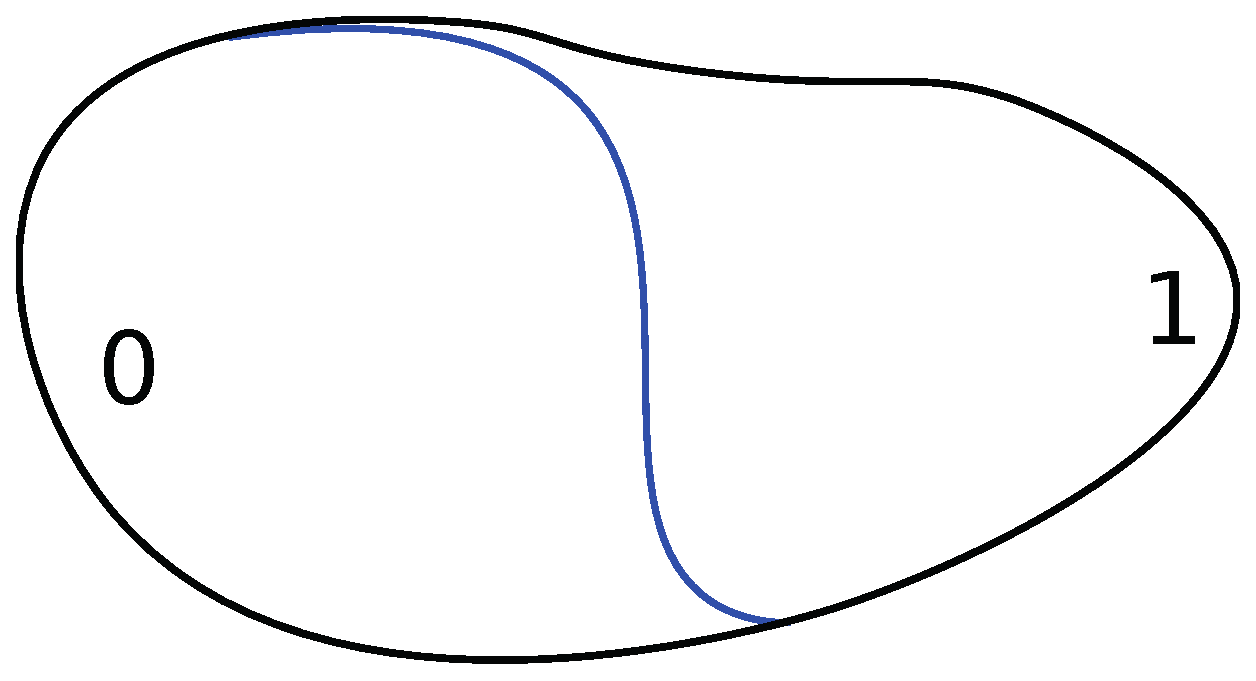
\includegraphics[width = 0.35\textwidth]{merge-opt2.eps}}\qquad \qquad 
	\subfloat[Merge partitions ${\cal P}$\label{fig:merge-nhood}]{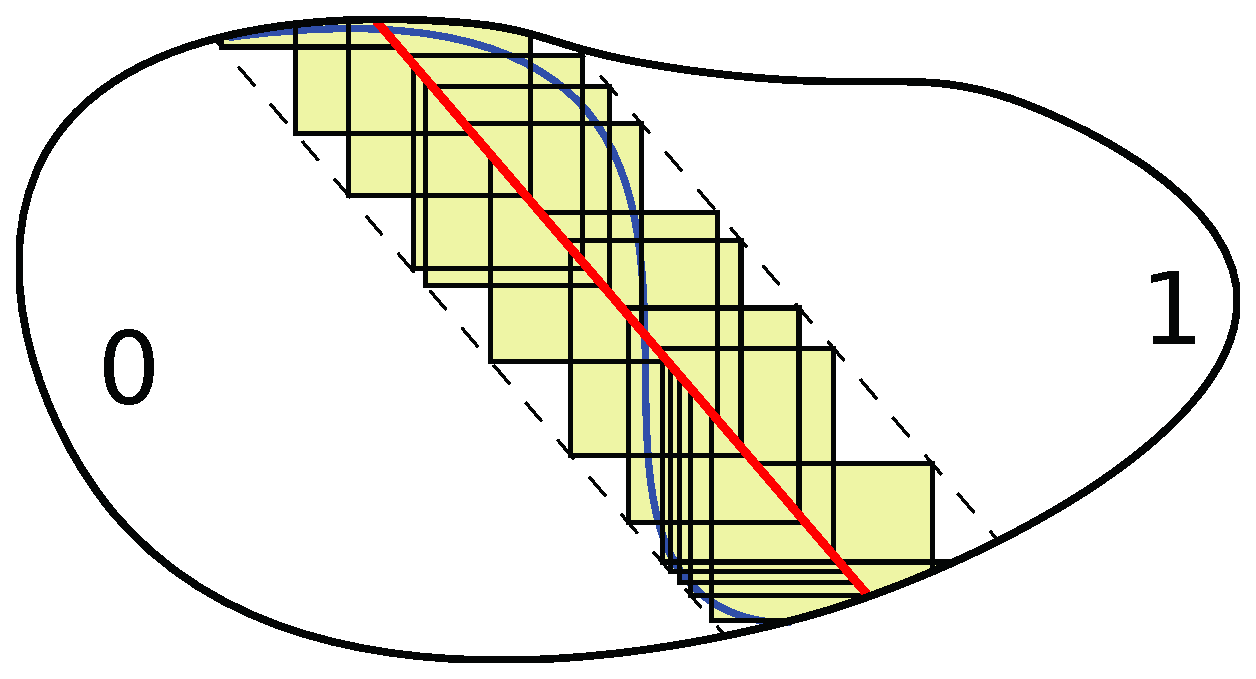
\includegraphics[width = 0.35\textwidth]{merge-nhood_red.eps}}\\ 
	\subfloat[Sub-problem solution $z^*$\label{fig:merge-sol}]{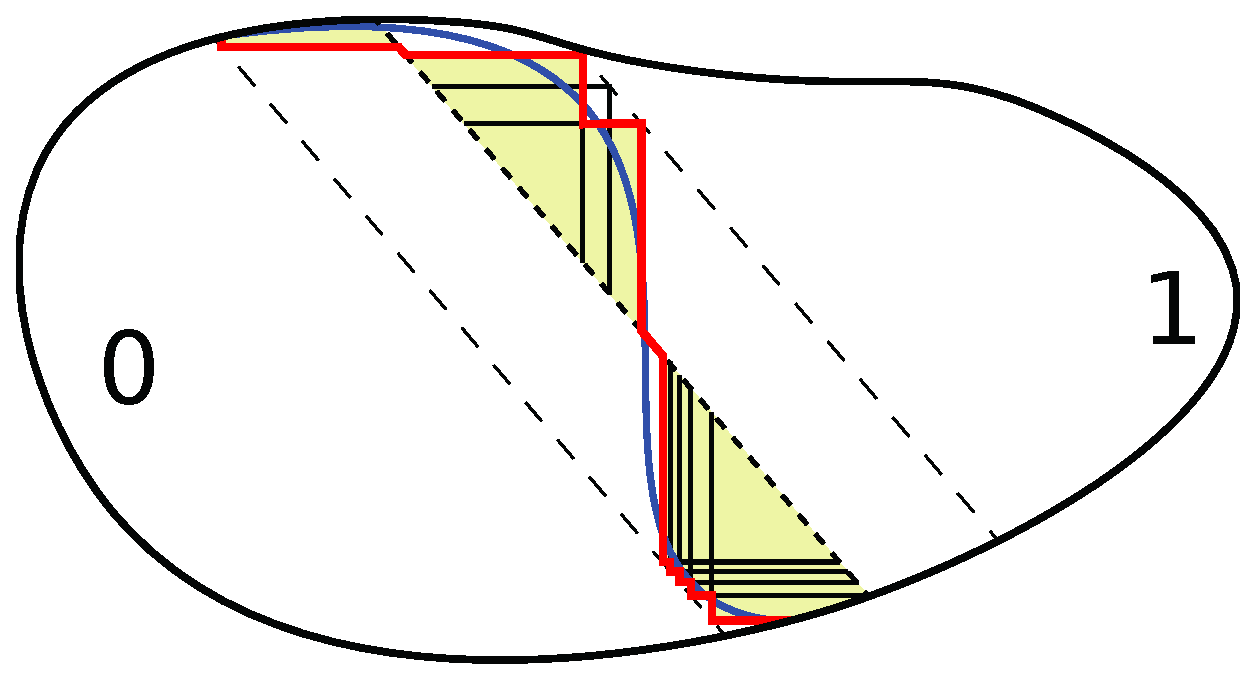
\includegraphics[width = 0.35\textwidth]{merge-sol.eps}}\qquad \qquad 
	\subfloat[Merged $f(x^k) \leq f(x^*)$\label{fig:merge-approx}]{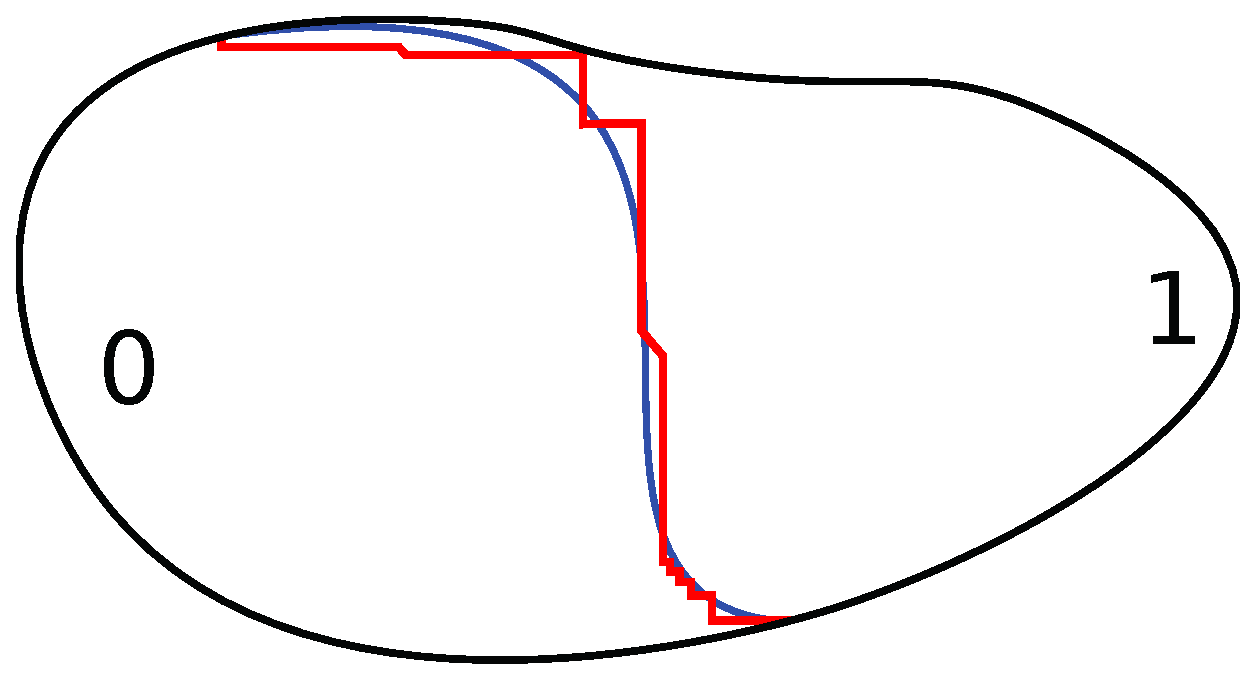
\includegraphics[width = 0.35\textwidth]{merge-approx.eps}}
	\caption[Solving the reduced subproblem gives an approximate solution to the master problem]{Solving the reduced subproblem induced by the merge partitions ${\cal P}$ to optimality, gives an approximate solution to the master problem.} 
    \label{fig:merge-solve}
\end{figure}

The partition on the decision variables representing the optimal solution $x^* \in {\cal F}$ is shown in blue in Figure~\ref{fig:merge-opt}. Figure~\ref{fig:merge-nhood} shows the merge partitions produced by merging the population $S$ and applying the random splitting heuristic. Here, the initial solution $x^{k-1}$ is the straight red partition boundary and each neighbouring solution in the population is represented by two triangular regions protruding from either side of this boundary. These regions represent the decision variables that take different values in the neighbouring solution, with respect to the initial --- regions on the left of the boundary indicate variables that have changed from 0 to 1 in the new solution, regions on the right indicate those that have changed from 1 to 0. The population is merged and split to produce the reduced subproblem which is expressed in terms of a set of partition variables $z$. This reduced subproblem is then solved using an exact solver or some other method. Figure~\ref{fig:merge-sol} shows that the optimal solution to the subproblem $z^*$ is a partition constructed from a subset of the boundaries of the merge partitions. Finally, $z^*$ is mapped back to a solution to the master problem $x^k$ (Figure~\ref{fig:merge-sol}), an approximation of $x^*$. If the stopping criteria is not yet met, then the merged solution $x^k$ is used as the initial solution for the next iteration.

Provided there is at least one feasible solution in the population at the time of merging, the merged solution $x^k$ will always be feasible. As the merge partitions are formed by the intersections of all the members in the population $S$ (and then randomly split), any solution $s_i \in S$ can be reconstructed by simply including all partitions that are associated with that solution. This is illustrated in Figure~\ref{fig:group_part} above, where $s_1$ can be constructed by the union of partitions $P_2 \cup P_3 \cup P_5 \cup P_6$. If $s_i$ is feasible, then the final merge operation is able to produce $s_i$ as $x^k$; meaning that, so long as the initial solution $x^{k-1}$ is feasible, $x^{k-1}$ will be a lower bound on the solution produced by merging and $f(x^{k-1}) \leq f(x^k) \leq f(x^*)$, even if the entire rest of the population consists of randomly generated bit strings, representing infeasible solutions.

% \begin{itemize}
% \item Neighbourhood Search (Step~\ref{step:nbhd}): This generates a population
%   of solutions for the merge step. While any heuristic method could be used
%   here, it will be assumed that it produces a randomised solution (so that the
%   solutions are nearly always different) and that the neighbourhood is sufficiently
%   large that the solutions produced will differ from the original $x^{k-1}$ in
%   several variables. The number of neighbouring solutions $m$ is an algorithm
%   parameter.
% \item Partitioning (Step~\ref{step:P}) can be implemented either by
%   starting with a single set $\{1,\ldots,n\}$ and iteratively partitioning it
%   where variables take on different values. Alternatively, we can define it
%   based on the unique set of solution values for $v\in\mathbb{R}^{|S|}$:
%   $P(v)=\{i\mid s_i = v_i\ \forall s\in S\}$ and $\mathcal{P}=\{P(v)\mid
%   P(v)\ne \emptyset\}$. At worst each set is a singleton, though in practice
%   we expect a quite small number of sets because (a) we are dealing with
%   combinatorial problems where most variables are either zero or one (or take
%   on a small number of values), and (b) the neighbourhood search tends to
%   generate a population of solutions with more similarity than just randomly
%   constructed solutions.
% \item Random Splitting (Step~\ref{step:RandSplit}) allows more control
%   over the size of $\mathcal{P}$ and hence the size of the problem solved in
%   the next step as typically $|\mathcal{P}|$ is quite small. Hence, this step creates 
%   a larger neighbourhood by carrying out random splitting of subsets. In fact it is
%   possible to run an extreme form of this algorithm with $m=0$ so that only
%   the random splitting in this step is used to define a neighbourhood. 
%   The choice of how to split subsets (perhaps with some biased randomisation) 
%   should be done in a problem dependent manner, as the choice of neighbourhood 
%   generated in this manner will clearly affect the effectiveness of the overall 
%   algorithm.
% \item Merging of solutions occurs in Step~\ref{step:merge}. It should be noted that this is
%   essentially a variant of the original problem but with significantly fewer
%   variables (one variable per $P\in\mathcal{P}$, $|\mathcal{P}|=K\ll n$). This
%   makes the step particularly amenable to use with integer or constraint
%   programming, where general purpose solvers generally cope well with small to
%   medium sized problems but solve times deteriorate rapidly as the problem
%   size increases. 
% \end{itemize}

\subsection{Properties of Merge Search}
There are some simple but important properties that follow directly from the way this matheuristic has been defined.

\begin{lemma}\label{thm:improve}
  The Merge Step~\ref{step:merge} produces a solution that is at least as good
  as any of the neighbours in $S$: $f(x^k) \ge f(s)\ \forall s\in S$
\end{lemma}
\begin{proof}
  By construction any solution $s\in S$ satisfies $s\in \mathcal{F}$ and
  $s_i=s_j$ $\forall i,j\in P\in\mathcal{P}$ and so is feasible for the
  optimisation problem in Step~\ref{step:merge}. Hence, $f(x^k)\ge f(s)$.
\end{proof}

\begin{corollary}\label{thm:hill-climb}
  Merge Search is a hill-climbing method that produces a non-decreasing sequence
 of solution values: $f(x^0)\le f(x^1)\le f(x^2)\le \ldots$
\end{corollary}

Hence, for diversification, the method relies entirely on the neighbourhood
search in Step~\ref{step:nbhd} of the algorithm and the randomised splitting in
Step~\ref{step:RandSplit}. This is not a problem for large instances such as
this, where simply finding a very good local minimum is already a very
challenging task. Furthermore, the following property holds:

\begin{lemma}\label{thm:optimal}
  For pure binary problems where all variables are $0-1$, if random splitting of subsets is used in Step~\ref{step:RandSplit} (allowing any possible split with some non-zero probability) with $K\ge 2^{m+2}$ then Algorithm~\ref{alg:MS} is guaranteed to converge to the optimal solution as the number of iterations approaches infinity. 
\end{lemma}
\begin{proof}
  By assumption there exists an optimal solution in $\cal F$, due to the existence of $x^0\in\cal F$ and boundedness of $\cal F$ when all variables are binary. Let $s^*$ be any optimal solution. The first thing to note is that if a partition $\mathcal{P}^*$ satisfies $s^*_i=s^*_j\ \forall P\in \mathcal{P}^*,\ i,j\in P$ then the Merge problem in Step~\ref{step:merge} yields and optimal solution. 
  Such a partition could be generated, from any arbitrary partition $\cal P$ by splitting each $P\in\cal P$ into $P_0=P\cap \{i\mid s^*_i=0\}$ and $P_1=P\cap \{i\mid s^*_i=1\}$. This splitting at most doubles the number of elements in the partition. \\
  Now the same argument can be used to show that $|\mathcal{P}|$ as produced in Step~\ref{step:P} has at most $2^{m+1}$ elements (corresponding to splitting based on solutions $s^1,\ldots,s^m$ and $x^{k-1}$). Hence, we only need $K$ to be at least $2^{m+2}$ to allow some chance of generating the required partition in any step. Hence, as the number of iterations of Algorithm~\ref{alg:MS} goes to infinity the chance of \emph{not} producing an optimal solution goes to zero. And of course, based on Corollary~\ref{thm:hill-climb} once an optimal solution has been found, the algorithm will not depart from this.
\end{proof}
While convergence to the optimal solution is of course extremely unlikely for practical sized instances, the lemma shows that it is at least theoretically possible. Furthermore, while $2^{m+2}$ appears quite large, the only real requirement is that $K$ is sufficiently large to allow each element of $\cal P$ to be split once, with $|\mathcal{P}|$ typically much smaller than $2^{m+1}$ in practice. Hence, while Merge Search is a hill-climbing method, it is at least in principle possible for the method to reach a global optimum from any starting point.


\subsection{Comparison with CMSA}
As mentioned previously, it may be noted here that this meta-heuristic has some similarity to the
recently published CMSA heuristic by~\citet{Blum2016}. Starting with an empty subinstance of the problem $\mathcal{C}^\prime$, solutions are probabilistically generated in this method, from scratch, and their components added to $\mathcal{C}^\prime$. This reduced subinstance is then solved using an exact solver and a so-called ``ageing'' mechanism is used to remove components from $\mathcal{C}^\prime$ that have not been useful in the preceding iterations. 

Although there are some similarities between Merge Search and CMSA, there are two areas where Merge Search diverges significantly from it. These are:
\begin{itemize}
\item the generation of candidate solutions to be merged; and
\item the aggregation of decision variables in the reduced subproblem.
\end{itemize}
The CMSA subproblems are still defined based on a population of solutions, however these solutions are constructed probabilistically, with each solution being generated from scratch. This has the two-fold effect of reducing the capacity of CMSA to learn from the best individual solution found so far, and also makes it impractical when trying to solve large-scale, or very complicated, problems for which constructing a feasible solution is extremely time consuming, such as the PCPSP that is considered here. Merge search avoids this issue by heuristically constructing an initial solution and then sampling its neighbourhood in order to generate a population, which is then used to define its subproblems. The effect of this is to make the time taken to generate the population of solutions dependent on the local search algorithm used to sample the neighbourhood of a given feasible solution which is often much faster than the algorithm used to find feasible solutions from scratch. Of course, this leaves Merge Search potentially susceptible to being overly sensitive to the quality of the initial solution --- as discussed previously in this section --- however, this can be mitigated by increasing the diversity of the population, or further splitting the merge partitions. 

The second area where there is a significant divergence between the two methods is in the aggregation of decision variables. CMSA uses its population of constructed solutions to determine the variables that are to be included in its reduced subproblem. If a variable is represented by an element of one of the candidate solutions in the population, it is automatically included in the reduced subproblem. These variables are added to the subproblem individually, and as such this aspect functions similarly to large neighbourhood search (LNS). One consequence of this is that the subproblems can become very large, especially for problems where there are naturally many non-zero values in a solution. To combat this, a so-called ``ageing'' mechanism is introduced in CMSA to ensure that elements that have not been useful in producing good quality solutions recently are removed from the pool of solution elements. In contrast, Merge Search uses information from across the entire population to determine which variables are added into the reduced subproblem as well as to aggregate variables that share common values across the population, and so likely share some kind of dependency. This grouping allows for more compact subproblems and a much larger region of the search space can be covered for the same computational power. The trade-off for this is much coarser-grained solutions, however this can be alleviated by the introduction of random splitting to these groups to help escape local optima.

% there are some significant differences. Most
% important is that the CMSA subproblems, while still defined based on a
% population of solutions, does not involve any aggregation of variables so that these
% subproblems can become very large unless the problem naturally has few
% non-zero values in the solution. Hence, the method as proposed in \cite{Blum2016}
% would be completely impractical for the problem considered here, because it has
% millions of non-zero variable values in solutions to large instances.
% Furthermore, CMSA relies on random construction to create populations of
% solutions, which reduces the ability to learn from the best solution found
% so far. The reliance purely on populations of feasible solutions (without the random splitting) also means that it relies purely on the random solution construction to escape any local optima. Finally, CMSA introduces an aging process to manage solution
% components, which is absent here.


\section{Applying Merge Search to solve problems}
Merge Search is presented here as a general hybrid meta-heuristic framework for solving constrained combinatorial optimisation problems. In order to demonstrate its effectiveness and versatility, Merge Search is applied to two problems from two different domains: the constrained pit-limit (CPIT) problem, an abstraction of a real-life problem from open-pit mining; and the Steiner tree problem in graphs (STPG), a famous NP-Complete problem which is very well-studied in the literature.

\subsection{Open-pit mining problems}
Open-pit mining is a very important industry in Australia and around the world~\citep{singh}. Two of the most critical tasks within the life-cycle of an open-pit mine is planning and production scheduling. These tasks allow the mine operator to estimate the total value of the mine over its life and also to identify areas for excavation that will yield the most value. Proper planning of a mine ensures maximum profit for the operator and, because this is typically talked about in the hundreds of millions of dollars, it is an excellent application for optimisation techniques as very small changes in efficiency can still translate to significant sums of money.\par

In order to model something so complex as a combinatorial optimisation problem, the earth to be mined (known as the \emph{orebody}) is typically discretised into a three-dimensional array of \emph{blocks} with each assigned a value based on the ore content and the cost required to excavate it. These values are calculated by taking core samples and using geological and statistical methods to estimate the value of each block. The aim is to maximise the net present value (NPV) of the mine by determining the set of blocks to extract and the order in which to extract them~\citep{Meagher2014}.\par

Problems in mine planning and production scheduling are very large and tend to have few side-constraints (often well under a hundred), but many blocks and many, many more precedence constraints governing when blocks can be mined. This means traditional mathematical solvers are unable to solve these problems without first using some form of decomposition, making these problems perfect candidates for hybrid meta-heuristics, despite there being very little in the literature.\par

Due to the sensitive nature of information surrounding mining enterprises, obtaining problem data for academic research can be challenging, however the website \emph{minelib}~\citep{espinoza_minelib:_2012} has a repository of problems and results that are freely available to the general public. These sets contain data for versions of the problem such as the ultimate pit limit (UPIT), constrained pit-limit and the precedence constrained production scheduling problem (PCPSP). It is the CPIT problem that will be the focus of these experiments.\par

\subsubsection{Solving CPIT with Merge Search}

\cite{Kenny:2017} describe a novel representation for the this type of problem and a greedy randomised adaptive search procedure (GRASP) algorithm for solving it. They build on this with local search operator for the CPIT problem, and use it in a simple merge search algorithm that operates without variable partitioning or random splitting~\citep{Kenny:2018}. By incorporating a variable partitioning mechanism, a much larger region of the search space is able to be explored for the same computational budget~\citep{Kenny:2019}. They exploit the structure of the problem, and treat many decision variables as a single group. This allows the size of the mixed-integer programming sub-problem to be greatly reduced and hence, the time required to solve it.\par

The algorithm presented in this paper is an exentsion of this work, with two additions: a random splitting heuristic, to allow greater granularity in the solutions produced; and a ``solution polishing'' technique, based on the local improvement heuristic from the GRASP algorithm.

\cmnt[angus]{is this enough information? should i include the pseudocode or something?}

\subsection{The Steiner tree problem in graphs}

The Steiner tree problem in graphs (STPG) is a classic problem in the field
of combinatorial optimisation, the decision version being one of the original 
21 NP-complete problems outlined by \cite{np:karp} in his seminal paper.
Aside from being a fundamental problem in the abstract world of computing theory, 
the STPG has numerous real-world applications in communications, pipeline and transport network
design, computational biology and very
large-scale integrated circuit (VLSI) design~\citep{vlsi:cho}.\par 
Despite being around for centuries~\citep{history:brazil}, the STPG has also gained
much attention in recent decades due to it being the mathematical structure behind 
multicast networking problems~\citep{steiner:hwang}. Exact methods for solving the STPG 
have been developed using techniques such as integer linear programming (ILP), 
lagrangian relaxation and primal-dual strategies~\citep{pd:polzin}; however these approaches suffer from
exponential worst-case computation times which can make some large-scale instances intractable. The current state-of-the-art 
exact approaches to solving the STPG are hybrid~\citep{algo:polzin,algo:daneshmand}; 
several algorithmic, graph reduction, metaheuristic and 
mathematical programming techniques, working together to produce provably optimal solutions
in a much faster time than traditional optimisation techniques alone.
When good quality, but not necessarily optimal, solutions are required in a reasonable amount of
time, metaheuristics and decomposition techniques have been used to tackle this problem; some of the
more successful approaches in this manner have been memetic algorithms \citep{memetic:klau}, ant colony optimisation
\citep{aco:singh,acogroup:nguyen}, local search techniques 
\citep{fastls:uchoa,effectivels:wade} and voronoi-based 
decomposition heuristics \citep{partition:leitner}.\par

The STPG is extremely well-travelled, with many sophisticated pre-processing techniques and methods of finding good quality solutions already available in the literature. The purpose of including it in this paper is not to improve the current state-of-the-art results; but to provide a simple test-bed, upon which the properties of the proposed merge search algorithm can be investigated --- much more easily than with a more complex, real-world problem such as the constrained pit-limit problem, mentioned above.

\subsubsection{Solving the STPG with Merge Search}

First described by \cite{kp:dowsland}, but subsequently used widely by 
many researchers, is the so-called key path neighbourhood.
A key path is defined as a path within a Steiner tree where the two end vertices are
either terminal vertices or vertices of degree at least 3; all intermediate 
vertices (if any) are of degree 2 and are not terminal. The useful property of such
structures is that their removal from a solution to the STPG will always result in two disconnected
trees which can then be subsequently reconnected. This local search neighbourhood was extended by~\cite{Kenny:2016}, by adding a so-called ``jump'' operator which aids in escaping local minima, and is used as the basis of the Merge Search algorithm presented in this paper.

The problem instance is first pre-processed using some of the techniques described in~\citet{pp:duin,pp:uchoa,stpg-reduce} to reduce the number of decision variables. An initial solution is constructed and a neighbouring population produced, using the methods described in~\cite{Kenny:2016}. This population of solutions is used to partition the decision variables in the manner described in Section~\ref{sec:MS}.

\begin{figure}[h]
\centering
\resizebox{0.60\linewidth}{!}{{}
    \includegraphics{stpg_merge.tikz}
    }
    \caption[Partitioning variables by merging solutions]{By merging two solutions (top left and right), the decision variables are partitioned into four disjoint sets, indicated here (bottom) by: red; blue; red and blue; and no colour.}\label{fig:stpg-partition} 
\end{figure}

These partitions can be split by selecting an arbitrary partition, and an arbitrary variable in that partition, and separating all variables representing vertices and edges that are connected to that arbitrary variable. This ensures that any partition is split such that all variables removed from the original partition comprise a connected sub-graph, and as such should be able to be included in the resultant merged solution on its own, without the original partition. If a partition is split such that all variables are separated, leaving the original partition empty, then the last variable added to the split is kept in the original partition. As the connected variables are added using DFS, this is always a variable on the boundary, and so this method will not suffer from the problems present with truely random splitting. 

Having partitioned and split the decision variables, the resulting reduced subproblem can be solved using a version of the~\cite{goemans} MIP formulation that has been modified be expressed in terms of a single set of partition variables, instead of edge and vertex variables.

\cmnt[angus]{should i actually include the formulation (or pseudocode) here?}

\section{Experiments}
This section details the experimental set up, the experiments performed and finally presents the results and discusses the implications those results suggest.
\subsection{Datasets}
\subsubsection*{The CPIT problem:}
Table~\ref{tab:datasets} details the properties of the problem instances used to test the algorithm in this paper. The instance name is given in the first column; followed by the number of blocks in the orebody model; the number of precedence arcs for each instance is provided in the third column; the fourth column gives the total number of time periods available; the number of decision variables is shown in the second last column; with the last column giving the total number of constraints in the problem model.\par
%
\begin{table}[h!]
\centering
\caption{Characteristics of \emph{minelib}~\citep{espinoza_minelib:_2012} datasets.}\label{tab:datasets}
% \begin{adjustbox}{width=0.48\textwidth}
\begin{tabular}{lrrrrr} \toprule
Instance & Blocks & Precedences & Periods & Variables & Constraints\\
\hline
\texttt{newman1} & 1,060 & 3,922 & 6 & 6,360 & 29,904\\
\texttt{zuck\_small} & 9,400 & 145,640 & 20 & 188,000 & 3,100,840\\
\texttt{kd} & 14,153 & 219,778 & 12 & 169,836 & 2,807,196\\
\texttt{zuck\_medium} & 29,277 & 1,271,207 & 15 & 439,155 & 19,507,290\\
\texttt{marvin} & 53,271 & 650,631 & 20 & 1,065,420 & 14,078,080\\
\texttt{zuck\_large} & 96,821 & 1,053,105 & 30 & 2,904,630 & 34,497,840\\
\bottomrule
\end{tabular}
% \end{adjustbox}
\end{table}
%
A few instances from the full \emph{minelib} dataset were omitted due to missing files, referencing more than two resources or being too large for the algorithm in its current incarnation.

\subsubsection*{The Steiner tree problem in graphs:}

The experiments were were carried out on categories $B$, $C$, $D$ and $E$ of the STPG problems from the \textit{steinlib} library~\citep{steinlib}, a standard dataset used by many researchers. The smaller-scale, category $B$ instances are 18 randomised networks with 50 to 100 vertices and 63 to 200 edges. The $C$ and $D$ datasets consists of 20 larger randomised networks, with 500 and 1,000 vertices, respectively, and between 625 to 25,000 edges. Finally, the $E$ dataset contains the largest instances, each with 2,500 vertices and between 3,125 and 62,500 edges. Details of the individual instances can be found in Table~\ref{tab:stpgprobs1}. 

The optimal solutions for these instances are reported in the library and 
have been proven by exact methods such as branch-and-bound with graph reduction techniques.\par

\begin{table}[h]
\centering
\caption[Characteristics of category $B$, $C$, $D$ and $E$ instances from the \textit{steinlib} database]{Characteristics of category $B$ and $C$ instances from the \textit{steinlib} database. $|V|$: number of vertices; $|E|$: number of edges; $|T|$: the number of terminals; and,
         opt: the total cost of the optimal solution.}\label{tab:stpgprobs1}
\begin{adjustbox}{width=\textwidth}
\begin{tabular}{lrrrr|lrrrr|lrrrr|lrrrr} \toprule
\multicolumn{5}{l}{Category $B$} & \multicolumn{5}{l}{Category $C$}&\multicolumn{5}{l}{Category $D$} & \multicolumn{5}{l}{Category $E$}\\ 
\cmidrule(lr){1-5} \cmidrule(lr){6-10}\cmidrule(lr){11-15}\cmidrule(lr){16-20}
Inst.&$|V|$&$|E|$&$|T|$&opt& Inst.&$|V|$&$|E|$&$|T|$&opt&Inst.&$|V|$&$|E|$&$|T|$&opt& Inst.&$|V|$&$|E|$&$|T|$&opt\\ \hline
$b01$ & 50 & 63 & 9 & 82 & $c01$ & 500 & 625 & 5 & 85&  $d01$ & 1,000 & 1,250 & 5 & 106 & $e01$ & 2,500 & 3,125 & 5 & 111\\
$b02$ & 50 & 63 & 13 & 83& $c02$ & 500 & 625 & 10 & 144&  $d02$ & 1,000 & 1,250 & 10 & 220 & $e02$ & 2,500 & 3,125 & 10 & 214\\
$b03$ & 50 & 63 & 25 & 138& $c03$ & 500 & 625 & 83 & 754&  $d03$ & 1,000 & 1,250 & 167 & 1,565& $e03$ & 2,500 & 3,125 & 417 & 4,013\\
$b04$ & 50 & 100 & 9 & 59& $c04$ & 500 & 625 & 125 & 1,079&  $d04$ & 1,000 & 1,250 & 250 & 1,935& $e04$ & 2,500 & 3,125 & 625 & 5,101\\
$b05$ & 50 & 100 & 13 & 61& $c05$ & 500 & 625 & 250 & 1,579&  $d05$ & 1,000 & 1,250 & 500 & 3,250& $e05$ & 2,500 & 3,125 & 1,250 & 8,128\\
$b06$ & 50 & 100 & 25 & 122& $c06$ & 500 & 1,000 & 5 & 55&  $d06$ & 1,000 & 2,000 & 5 & 67& $e06$ & 2,500 & 5,000 & 5 & 73\\
$b07$ & 75 & 94 & 13 & 111& $c07$ & 500 & 1,000 & 10 & 102&  $d07$ & 1,000 & 2,000 & 10 & 103& $e07$ & 2,500 & 5,000 & 10 & 145\\
$b08$ & 75 & 94 & 19 & 104& $c08$ & 500 & 1,000 & 83 & 509&  $d08$ & 1,000 & 2,000 & 167 & 1,072& $e08$ & 2,500 & 5,000 & 417 & 2,640\\
$b09$ & 75 & 94 & 38 & 220& $c09$ & 500 & 1,000 & 125 & 707&  $d09$ & 1,000 & 2,000 & 250 & 1,448& $e09$ & 2,500 & 5,000 & 625 & 3,604\\
$b10$ & 75 & 150 & 13 & 86& $c10$ & 500 & 1,000 & 250 &1,093&  $d10$ & 1,000 & 2,000 & 500 & 2,110& $e10$ & 2,500 & 5,000 & 1,250 &5,600\\
$b11$ & 75 & 150 & 19 & 88& $c11$ & 500 & 2,500 & 5 &32&  $d11$ & 1,000 & 5,000 & 5 & 29& $e11$ & 2,500 & 12,500 & 5 &34\\
$b12$ & 75 & 150 & 38 & 174& $c12$ & 500 & 2,500 & 10 & 46&  $d12$ & 1,000 & 5,000 & 10 & 42& $e12$ & 2,500 & 12,500 & 10 & 67\\
$b13$ & 100 & 125 & 17 & 165& $c13$ & 500 & 2,500 & 83 & 258&  $d13$ & 1,000 & 5,000 & 167 & 500& $e13$ & 2,500 & 12,500 & 417 & 1,280\\
$b14$ & 100 & 125 & 25 & 235& $c14$ & 500 & 2,500 & 125 & 323&  $d14$ & 1,000 & 5,000 & 250 & 667& $e14$ & 2,500 & 12,500 & 625 & 1,732\\
$b15$ & 100 & 125 & 50 & 318& $c15$ & 500 & 2,500 & 250 & 556&  $d15$ & 1,000 & 5,000 & 500 & 1,116& $e15$ & 2,500 & 12,500 & 1,250 & 2,784\\
$b16$ & 100 & 200 & 17 & 127& $c16$ & 500 & 12,500 & 5 & 11&  $d16$ & 1,000 & 25,000 & 5 & 13& $e16$ & 2,500 & 62,500 & 5 & 15\\
$b17$ & 100 & 200 & 25 & 131& $c17$ & 500 & 12,500 & 10 & 18&  $d17$ & 1,000 & 25,000 & 10 & 23& $e17$ & 2,500 & 62,500 & 10 & 25\\
$b18$ & 100 & 200 & 50 & 218& $c18$ & 500 & 12,500 & 83 & 113&  $d18$ & 1,000 & 25,000 & 167 & 223& $e18$ & 2,500 & 62,500 & 417 & 564\\
&&&&& $c19$ & 500 & 12,500 & 125 & 146 &$d19$ & 1,000 & 25,000 & 250 & 310& $e19$ & 2,500 & 62,500 & 625 & 758\\
&&&&& $c20$ & 500 & 12,500 & 250 & 267 &$d20$ & 1,000 & 25,000 & 500 & 537& $e20$ & 2,500 & 62,500 & 1,250 & 1,342\\
\bottomrule
\end{tabular}
\end{adjustbox}
\end{table}

\subsection{Pre-processing}
\subsubsection*{The CPIT problem}
The ``time-expanded'' method of representing the CPIT problem given in~\cite{Kenny:2017} has one significant drawback: it exponentially increases the size of the problem instances. In this technique, each block-time pair is associated with a single decision variable and a solution is represented as a closure which partitions this expanded graph. In order to mitigate this effect, the structure of the problem can be exploited to apply pre-processing to reduce the number of variables and constraints in each problem instance.

First, a relaxed version of the problem, called UPIT, is solved to determine the set of blocks that are worth extracting at all; then the earliest and latest possible times for extraction for each block are computed. Because a condition of extracting a block is that all blocks above it must be extracted first, blocks that are deep cannot be extracted too early in the process --- because there is not enough time to reach them --- and similarly, blocks that are close to the surface cannot be extracted too late --- as there will not be enough time to reach the blocks below. More detail about these pre-procesing methods can be found in~\cite{Kenny:2017}.

\subsubsection*{The Steiner tree problem in graphs}
There are many techniques available in the literature for pre-processing instances of the STPG, ranging from the very simple to the very complicated. As the experiments on the STPG for this study were not intended to improve the current state-of-the-art, but merely to investigate the properties of merge search and prove its versatility; the purpose of pre-processing the problem instances was simply to make them more manageable for the algorithms being tested. To this end, three basic ones were chosen from the literature: removing non-terminal vertices of degree 1; removing edges where a shorter path exists in the graph; and, replacing the edges incident to non-terminal vertices of degree two with a single edge. For further reading on graph reduction techniques for pre-processing instances of the STPG, see \cite{pp:duin,pp:uchoa,stpg-reduce}.

\subsection{Experimental setup}
The experiments were carried out on an \emph{Intel{\textsuperscript{\textregistered}} Core{\textsuperscript{TM}} i5-2320} processor (3.0GHz) with 24GB RAM running Linux. All code was implemented in C++ with GCC-4.8.0. CPLEX Studio 12.7, operating with a single thread due to the need for callbacks, was employed as the mixed integer programming (MIP) solver. For the CPIT problem experiments, the boost library implementation of the Boykov-Kolmogorov algorithm was used to solve the UPIT sub-problem during the pre-processing stage.

\subsubsection*{The CPIT problem:}
The merge search algorithm was compared against the baselines of the results published on the \emph{minelib}~\citep{espinoza_minelib:_2012} website and the results from using a greedy randomised adaptive search procedure (GRASP) heuristic for the precedence constrained production scheduling problem (PCPSP)~\citep{Kenny:2017}, adapted for use with the CPIT problem. Also provided are the results for a variant of the merge search algorithm that uses variable grouping but no random splitting, previously published in~\cite{Kenny:2018} --- these results are included in order to illustrate the effect that random splitting has on solution quality. 

Each algorithm was run 20 times on each instance, recording the mean objective value and standard deviation of the resulting solution produced by each run. Finally, the last experiment performed was to use the local improvement heuristic from the GRASP algorithm to ``polish'' the best result produced by the merge algorithm.

\subsubsection*{The Steiner tree problem in graphs:}
The merge search algorithm was compared against three separate baseline algorithms, the greedy randomised adaptive search (GRASP) heuristic, pure local search and pure MIP. The method of constructing initial solutions was different between the GRASP and merge search algorithms, so pure local search and pure MIP were included to ensure any improvement was not solely based on this factor. Aside from population merging, the merge search algorithm comprises two main components, local search and MIP search; so by isolating these two factors, it can be shown that merge search is greater than the sum of its parts.

Each algorithm was run 30 times on each (pre-processed) instance from the datasets, recording the mean objective value and standard deviation across all of the runs. All instances in the datasets used are supplied with their optimal objective values and this is used for the main stopping criteria. Otherwise, the stopping criteria of the merge search algorithm is generally dictated by the number of seconds spent in the MIP search so the time taken for each search is not provided, as it does not give much information about the performance of the algorithm. However, special mention is made when the algorithm terminated early for all runs.

Additional experiments were performed to investigate the difference between using the random and deterministic solution construction heuristics and the effect of population size on the size of the reduced sub-problem. In order to preserve space, a representative subset of the problem instances is used to illustrate the outcome of these experiments; however, these results are not ``cherry-picked'' and the full tables are available in the appendix. 
\cmnt[angus]{(will add appendix later)}
\cmnt[angus]{should i add some details about the parameters used here?}

\section{Results and discussion}
\subsection{The CPIT problem:}
Table~\ref{tab:mine:main} provides the results of the three algorithms tested on the six problem instances from the \emph{minelib} dataset, along with the linear programming (LP) upper bound and the current best solution as published on the \emph{minelib} website, ordered from smallest problem instance to largest.

In this table, it can be seen that the two merge search algorithms consistently produce better results than the \emph{minelib} and the GRASP heuristic results, except for \newman{} and \zucklarge{}. The results for \newman{} are similar because the problem instance is so small and it can be assumed that the objective value of 2.418E+07 is quite close to the optimal solution, as all three algorithms agree on this as an average value and when the search is performed without any stopping criteria, the maximum objective value that is found is 2.41798E+07.

\begin{table}[h!]
\centering
\caption[Results on \emph{minelib} dataset instances]{Results on \emph{minelib} dataset instances. Given are the LP upper bound, current best solution from the \emph{minelib} website, the mean objective values (\(\mu\)) and standard deviations (\(\sigma\)) for the GRASP heuristic, merge search without random splitting and full merge search heuristic.% The final column gives the result of using the local improvement heuristic from the GRASP algorithm to polish the best solution found with merge search.
}\label{tab:mine:main}
\begin{adjustbox}{width=\textwidth}
\begin{tabular}{lrrrrrrrrrr} \toprule
 & \multicolumn{1}{c}{LP UB} & \multicolumn{1}{c}{\emph{minelib}} & \multicolumn{2}{c}{GRASP heuristic} & \multicolumn{2}{c}{merge search (no splitting)} & \multicolumn{2}{c}{merge search (with splitting)}\\
\cmidrule(lr){2-2}\cmidrule(lr){3-3} \cmidrule(lr){4-5} \cmidrule(lr){6-7} \cmidrule(lr){8-9}
Instance & & & \multicolumn{1}{c}{\(\mu\)}&\multicolumn{1}{c}{\(\sigma\)} & \multicolumn{1}{c}{\(\mu\)}&\multicolumn{1}{c}{\(\sigma\)}  \\ \midrule
%
\input ../mine/tables/main_table.tex
%
\bottomrule

% \multicolumn{5}{l}{$^*$ this result was beaten by polishing the best merge search solution with the GRASP local improvement heuristic (Table~\ref{tab:mine:polish}).}
\end{tabular}
\end{adjustbox}
\end{table}
Comparing the results of the two variants of merge search illustrates the effect that random splitting has on the quality of the solution produced. For smaller problem instances, the two algorithms produce very similar quality solutions, indicating that the random splitting has little effect. 
\footnotetext{{This result was beaten by polishing the best merge search solution with the GRASP local improvement heuristic (Table~\ref{tab:mine:polish}).}}% footnote mark is in table source
However, as the size of the problem increases, the effect of the random splitting becomes more pronounced, with the biggest effect being on the two largest instances \zuckmed{} and \zucklarge{}\footnote{Although it is technically a larger problem than \zuckmed, solving the UPIT problem on the \marvin{} instance, as part of the pre-processing stage, eliminates many blocks and makes its effective size much smaller than \zuckmed.}. 

If there are no overlaps at all between variables across solutions, then the partitions in the reduced sub-problem are simply the set differences of the variables in each solution and the seed solution. In this extreme case, the merge operation is unable to produce a solution that does not already exist in the population, unless some random splitting of the partitions is performed. As the size of the problem instance decreases, the likelihood that there will be overlaps between variables across solutions increases. These overlaps in the variable sets produce splits in the partitions when producing the reduced sub-problem, reducing the need for additional random splitting to produce a different solution to those already existing in the generated population. This is not to suggest that random splitting would not be beneficial; but the problem with random splitting is that it is \emph{random}, and there is no way of guaranteeing that a particular split will improve the quality of a solution after merging, any more than a split produced by overlapping variable sets will.

The GRASP heuristic produces consistently worse results than merge search. This is expected as the sliding window heuristic used in the local improvement phase of the algorithm is better suited to incrementally improving a good solution than turning a mediocre solution into a good one, as it only operates on a small subset of the variables at one time. This means that it is good for ``tweaking'' a solution by shifting the time that a block is mined forward or backward one or two periods; but it is no good if the time that the block is mined must be moved by many periods, as this would take a lot of passes to achieve.

\subsubsection*{Convergence behaviour}

This idea of GRASP being better suited to incrementally improving an already good solution is demonstrated in Figure~\ref{plot:mine:runtime}. This figure gives the plots of the convergence behaviour of both the GRASP algorithm and merge search on all six of the CPIT instances. It can be seen in these plots that merge search converges quicker in nearly all instances, except for \dmine{}. 

\begin{figure}[!]
    \centering
    \begin{subfigure}[t]{0.4\textwidth}
    \centering
    \resizebox{\linewidth}{!}{
    \includegraphics{mine/plots/conv/newman1_conv.tikz}
    }
    \vspace*{-5mm}\caption{\newman{}}
    \label{plot:newman-conv}
    \end{subfigure}
    \quad
    \begin{subfigure}[t]{0.4\textwidth}
    \centering
    \resizebox{\linewidth}{!}{
    \includegraphics{mine/plots/conv/zuck_small_conv.tikz}
    }
    \vspace*{-5mm}\caption{\zucksmall{}}
    \label{plot:zuck-small-conv}
    \end{subfigure}
    %
    \\[5mm]
    %
    \centering
    \begin{subfigure}[t]{0.4\textwidth}
    \centering
    \resizebox{\linewidth}{!}{
    \includegraphics{mine/plots/conv/kd_conv.tikz}
    }
    \vspace*{-5mm}\caption{\dmine{}}
    \label{plot:kd-conv}
    \end{subfigure}
    \quad
    \begin{subfigure}[t]{0.4\textwidth}
    \centering
    \resizebox{\linewidth}{!}{
    \includegraphics{mine/plots/conv/zuck_med_conv.tikz}
    }
    \vspace*{-5mm}\caption{\zuckmed{}}
    \label{plot:zuck-med-conv}
    \end{subfigure}
    %
    \\[5mm]
    %
    \centering
    \begin{subfigure}[t]{0.4\textwidth}
    \centering
    \resizebox{\linewidth}{!}{
    \includegraphics{mine/plots/conv/marvin_conv.tikz}
    }
    \vspace*{-5mm}\caption{\marvin{}}
    \label{plot:marvin-conv}
    \end{subfigure}
    \quad
    \begin{subfigure}[t]{0.4\textwidth}
    \centering
    \resizebox{\linewidth}{!}{
    \includegraphics{mine/plots/conv/zuck_large_conv.tikz}
    }
    \vspace*{-5mm}\caption{\zucklarge{}}
    \label{plot:zuck-large-conv}
    \end{subfigure}
    \caption[Convergence plots for merge search on CPIT instances]{Convergence plots for merge search on CPIT instances. Merge search data is shown in blue and GRASP is shown in red.}
    \label{plot:mine:runtime}
\end{figure}

The difference here, is that the initial solution is already quite close in value to the resultant solution, so there are not a lot of improvements that can be made. This means that the more exhaustive search for small improvements of the GRASP algorithm is more likely to be effective, early on, than the more global search of the merge search algorithm, which relies on the stochastic natures of the local search operator and arbitrary splitting heuristic to find its improvements. Merge search does get there in the end --- and manages to find a slightly better solution in this case --- but it takes longer and with a more gentle curve. For all the other instances, where the gap between the initial solution and the resultant one is much larger, merge search is demonstrably more suited to the task.

It can also be seen from these plots that once the algorithm has seemingly converged, it can sometimes find a way out of the local optima and find a much better solution. This is evidenced in the plots for \zuckmed{}~(Figure ~\ref{plot:zuck-med-conv}), \marvin{}~(Figure~\ref{plot:marvin-conv}) and also Figure~\ref{plot:polish.med1} below. This behaviour is expected in such large problem instances, as once it has started to converge there are many ways to make the solution worse, but only a few to make it better; but once it has found a way out of the local optima, often several other improving moves will become apparent as well.

\subsubsection*{Runtime information}

Table~\ref{tab:mine:runtime} gives the runtime information (wall time and CPU time) for both the GRASP and merge search algorithms. As they use a MIP solver to solve their restricted sub-problems, the runtime of both GRASP and merge search is reasonably easily configured by controlling how long the solver is allowed to run for each iteration. The parameters of the GRASP algorithm were chosen so that the search would take roughly the same amount of time as that of the merge search --- and for the most part, they are pretty similar. 

\begin{table}[h!]
\centering
\caption[Runtime information for experiments on CPIT]{Runtime information for experiments on CPIT. Given are the mean (\(\mu\)) and standard deviations (\(\sigma\)) of the wall and CPU time for the GRASP and merge search algorithms, in seconds.}\label{tab:mine:runtime}
\begin{adjustbox}{width=0.7\textwidth}
\begin{tabular}{lrrrrrrrr} \toprule
 & \multicolumn{4}{c}{GRASP} & \multicolumn{4}{c}{merge search}\\
\cmidrule(lr){2-5} \cmidrule(lr){6-9}
 & \multicolumn{2}{c}{Wall time [s]} & \multicolumn{2}{c}{CPU time [s]} & \multicolumn{2}{c}{Wall time [s]} & \multicolumn{2}{c}{CPU time [s]}\\
\cmidrule(lr){2-3}\cmidrule(lr){4-5} \cmidrule(lr){6-7}\cmidrule(lr){8-9}
Instance & \multicolumn{1}{c}{\(\mu\)}&\multicolumn{1}{c}{\(\sigma\)} & \multicolumn{1}{c}{\(\mu\)}& \multicolumn{1}{c}{\(\sigma\)}& \multicolumn{1}{c}{\(\mu\)}&\multicolumn{1}{c}{\(\sigma\)} & \multicolumn{1}{c}{\(\mu\)}& \multicolumn{1}{c}{\(\sigma\)}\\ \midrule

\input ../mine/tables/runtime_table.tex

\bottomrule
\multicolumn{9}{l}{\(^*\)population size for \zucklarge{} set at 500 for merge search due to insufficient memory.}
\end{tabular}
\end{adjustbox}
\end{table}

The two instances that are significantly different in runtime between GRASP and merge search are \dmine{} and \zucklarge{}. The reason that \zucklarge{} is so different is that it was impossible to run the merge search algorithm with a population of 1,000 on such a large problem instance, due to memory issues (even with 23 GB of RAM!); so a smaller population size of 500 was used, which took much less time to produce and to compute the merge partitions.

The reason for the differences in runtime on \dmine{} is illustrated in Figure~\ref{plot:mine:time}.
%
\begin{figure}[h!]
    \centering
    \begin{subfigure}[t]{0.4\textwidth}
    \centering
    \resizebox{\linewidth}{!}{
    \includegraphics{mine/plots/time/zuck_small_grasp_time.tikz}
    }
    \caption{}
    \label{plot:time.1}
    \end{subfigure}
    \quad
    \begin{subfigure}[t]{0.4\textwidth}
    \centering
    \resizebox{\linewidth}{!}{
    \includegraphics{mine/plots/time/zuck_small_merge_time.tikz}
    }
    \caption{}
    \label{plot:time.2}
    \end{subfigure}
    \caption[Plot of wall time {[s]} for \zucksmall{} and \dmine{} instances]{Plot of wall time [s] for \zucksmall{} (red) and \dmine{} (blue) instances. Sub-figure (\subref{plot:time.1})~shows GRASP algorithm data and (\subref{plot:time.2})~shows merge search data.}
    \label{plot:mine:time}
\end{figure}
%
This figure shows plots of the amount of wall time in seconds consumed per iteration of the respective algorithms. The GRASP algorithm is measured by ``window movements'', which counts the number of times the window has incremented forwards or backwards along the solution. The merge search algorithm is measured by iterations; each the time for each iteration is measured at the point when a new candidate solution is generated for the population, so it is clear to see that, with a population size of one thousand, every thousandth iteration will include an extra amount of time to include the merge operation itself. 

It is important to remember here that the \dmine{} instance only has a maximum of 12 periods allowed, while \zucksmall{} has 20. So the difference in time between GRASP and merge search is easy to explain, because GRASP is dependent on the number of periods in the solution as that determines how many window movements will be made; whereas merge search will generate the same size population and perform the same number of merges, no matter how many periods are allowed. This is demonstrated very clearly in Figure~\ref{plot:time.2}, where there is very little difference between the two instances. It can be seen that the population is generated reasonably quickly (indicated by the flat parts of the curve) and then each point where there is a sudden jump in the amount of time taken indicates that a merge operation has taken place.

But this is not the end of the story. In these two examples, GRASP took 2,979 seconds to complete the search on \dmine{} and it took 4,180 to complete the search on \zucksmall{}. If there was a direct linear relationship between time taken to complete the search and number of periods, the amount of time GRASP should take to complete its search on \zucksmall{} should be \(\frac{2,979\times20}{12} = 4,965\). So where did the other 13 minutes go?

Looking at Figure~\ref{plot:time.1}, the main thing that can be noticed here is that the shape of the plot for \zucksmall{} is significantly different to the shape of the plot for \dmine{}. The regular flat spots in the plot for \zucksmall{} indicate that there is a group of periods for that problem that are not used by the solution, or do not contain any blocks that can be moved around, and therefore the MIP solver will not take the full amount of allowed time to solve the reduced sub-problem. It so happens that the solution to \zucksmall{} does not use any period after period 16, so the first and last few window moves of each full pass take very little time at all. In contrast the \dmine{} instance uses periods right up until period 10, so there are fewer window moves that will be skipped over, as evidenced by the straighter line on the plot.

\subsubsection*{Solution polishing}

As the quality of the solutions produced by the random construction heuristic is not extremely high, too much of the local improvement phase is spent moving the times that blocks are mined over long temporal distances; so the algorithm is unable to produce high quality solutions in the allowed computational budget. It was observed however, that the quality of the solutions produced by the GRASP algorithm greatly depended on the quality of the initial solution that was constructed. So it was decided to see what would happen if the local improvement heuristic from the GRASP algorithm was applied to ``polish'' the best solution obtained by the merge search algorithm. These results are given in Table~\ref{tab:mine:polish}.

\begin{table}[h!]
\centering
\caption[Results of polishing the best merge search solution]{Results of polishing the best merge search solution with the local improvement heursistic from the GRASP algorithm. Given is the LP upper bound and current best solution from the \emph{minelib} website, the objective value of the best solution produced by the merge search algorithm and the value of that solution when polished by the local improvement heuristic.}\label{tab:mine:polish}
\begin{adjustbox}{width=0.6\textwidth}
\begin{tabular}{lrrrr} \toprule
Instance & \multicolumn{1}{c}{LP UB} & \multicolumn{1}{c}{\emph{minelib}} & \multicolumn{1}{c}{merge search} & polished merge\\ 
\midrule
%
\input ../mine/tables/polish_table.tex
%
\bottomrule
\end{tabular}
\end{adjustbox}
\end{table}

This table clearly demonstrates that the sliding window heuristic is very effective in improving solutions produced by merge search, even surpassing the \emph{minelib} result for \zucklarge{} --- something that merge search could not achieve on its own, without polishing. For these experiments, the best solution from the merge search runs is taken and then three passes of the sliding window heuristic is applied. Although doing this effectively increases the allowed computational budget, the quality of the solutions produced by doing this is better than if the computational budget is increased for either of the two algorithms on their own. In the case of the GRASP algorithm, the quality of the solution at the end of its run is still too low to be able to improve the objective value by very much in only three passes. In the case of the merge search algorithm, because both the population generation and merge partition splitting occurs stochastically, as the quality of the solution increases the chances of finding an improving solution, or partition split, by chance decreases. This means that the search is likely to have converged by the end of its run, so increasing the computational budget at this point is unlikely to produce much of an improvement in the quality of the solution, if any at all.

Applying the sliding window heuristic at the end of the merge search process solves both of these problems. The sliding window heuristic performs a much more methodical and exhaustive search to find small improvements that can be made to the solution which might be difficult to find by random sampling, in such a large search space. Additionally, by starting the sliding window heuristic with a much higher quality initial solution, computational effort does not need to be wasted on the ``low hanging fruit'' that can be found easily by sampling the search space. As the heuristic only considers a small subset of the variables at a time, it cannot make large changes to the solution in a single iteration. 

\begin{figure}[t!]
    \centering
    \begin{subfigure}[t]{0.4\textwidth}
    \centering
    \resizebox{\linewidth}{!}{
    \includegraphics{mine/plots/polish/zuck_med_polish.tikz}
    }
    \vspace*{-5mm}\caption{Merge with polishing on \zuckmed{}}
    \label{plot:polish.med1}
    \end{subfigure}
    \quad
    \begin{subfigure}[t]{0.4\textwidth}
    \centering
    \resizebox{\linewidth}{!}{
    \includegraphics{mine/plots/polish/zuck_med_grasp_polish.tikz}
    }
    \caption{Detail of polishing phase}
    \label{plot:polish.med2}
    \end{subfigure}
    %
    \\[5mm]
    %
    \centering
    \begin{subfigure}[t]{0.4\textwidth}
    \centering
    \resizebox{\linewidth}{!}{
    \includegraphics{mine/plots/polish/zuck_large_polish.tikz}
    }
    \vspace*{-5mm}\caption{Merge with polishing on \zucklarge{}}
    \label{plot:polish.large1}
    \end{subfigure}
    \quad
    \begin{subfigure}[t]{0.4\textwidth}
    \centering
    \resizebox{\linewidth}{!}{
    \includegraphics{mine/plots/polish/zuck_large_grasp_polish.tikz}
    }
    \vspace*{-5mm}\caption{Detail of polishing phase}
    \label{plot:polish.large2}
    \end{subfigure}
    \caption[Plot of merge search with solution polishing on \zuckmed{} and \zucklarge{} instances]{Plot of merge search with solution polishing on \zuckmed{} (top) and \zucklarge{} (bottom) instances. The left-hand figures show the entire merge search (blue) and polishing (red) phases; the right-hand figures show details of the polishing phases.}
    \label{plot:mine:polish}
\end{figure}

Figure~\ref{plot:mine:polish} contains plots that illustrate this concept on two instances of the CPIT problem, \zuckmed{} and \zucklarge{}. The left-hand sub-figures show the full process with both merge phase (shown in blue) and polishing phase (shown in red). Figure~\ref{plot:polish.med1} demonstrates the power of intensification of the search with the sliding window heuristic. Here, the blue merge plot can seen to have effectively converged as there has been no significant improvement in objective value for over half an hour of wall time. Applying the sliding window heuristic to this ``converged'' solution results in an almost immediate improvement, followed by subsequent improvements, before this too converges to its local optimum.

Not as emphatic in demonstrating this point are the results presented in Figure~\ref{plot:polish.large1}. It can be seen in this figure that merge search was still a ways off from converging, although it had started to slow its progress. It could be argued that, were merge search allowed to continue, it would have found the same solution eventually. Although, it can be seen in the plot that applying the polishing heuristic to this unconverged solution did still result in an initial rapid increase in solution quality; and as merge search was beginning to tail off, it probably would have taken longer to reach its goal.

The results from these experiments suggest that, while merge search is adept at finding a good quality global solution, it benefits from the addition of a more exhaustive local method to intensify its search. 

\subsubsection*{Updated state-of-the-art results}

When this research was first undertaken, the current published state-of-the-art results were indeed those available on the \emph{minelib} website. However, since then, there have been several developments as published in a recent paper by~\cite{minelib-improved} that has collated all reported improvements to the \emph{minelib} dataset.

According to this aggregation of results, recently there are three separate studies that have improved the most on the \emph{minelib} results for the CPIT problem instances used for this research~\citep{newman-improved,zuck-small-improved,JELVEZ20161169}. These improved results are given in Table~\ref{tab:mine:update} in terms of their LP gap, and are compared with the original \emph{minelib} results and the polished merge results from earlier in this section.

\begin{table}[h!]
\centering
\caption[Recent updates to state-of-the-art results for \emph{minelib} CPIT instances]{Recent updates to state-of-the-art results for \emph{minelib} CPIT instances. Given is the percentage gap between the LP upper bound and the best result achieved for each respective study, compared with the original \emph{minelib} results and the best results from this research.}\label{tab:mine:update}
\begin{adjustbox}{width=0.6\textwidth}
\begin{tabular}{lrrrrr} \toprule
& & & & \multicolumn{2}{c}{new results}\\ 
\cmidrule(lr){5-6}
Instance & \multicolumn{1}{c}{LP UB} & \multicolumn{1}{c}{\emph{minelib}} & \multicolumn{1}{c}{polished merge} & \multicolumn{1}{c}{publication} & \multicolumn{1}{c}{gap}\\ 
\midrule
%
\input ../mine/tables/updated_table.tex
%
\bottomrule
\end{tabular}
\end{adjustbox}
\end{table}

Although the results from this study do not improve on every known bound in the literature, they certainly are competitive with the state-of-the-art and actually do improve the current best-known bound for the \dmine{} and the \zucklarge{} instances.

\subsection{The Steiner tree problem in graphs:}

\begin{table}[h]
% \begin{sidewaystable}
\centering
\caption[Results on \emph{steinlib} dataset \(B\) instances]{Results on \emph{steinlib} dataset \(B\), \(C\), \(D\) and \(E\) instances. Given are the known optimal solutions and mean objective values and standard deviations for pure local search, pure MIP, GRASP heuristic and merge search heuristic. Algorithms which managed to find the optimal solution in at least one of its runs are indicated by \opt{} next to the objective value.}\label{tab:stpg:results}
% \begin{adjustbox}{width=\textwidth}
\begin{tabular}{cc}
% \begin{table}[h!]
\centering
% \caption{Results on \emph{steinlib} dataset \(C\) instances, investigating the difference between the deterministic and random construction heuristics. Given are the average objective value and standard deviation for solutions produced by both heuristics over 20 runs and the difference between the averages, expressed as a percentage.}\label{tab:stpg:init:b}
% \begin{adjustbox}{width=\textwidth}
\begin{adjustbox}{width=0.48\textwidth}
\begin{tabular}{lrrrrrrrrr} \toprule
 &  & \multicolumn{2}{c}{pure LS} & \multicolumn{2}{c}{pure MIP} & \multicolumn{2}{c}{GRASP} & \multicolumn{2}{c}{merge search}\\
\cmidrule(lr){3-4} \cmidrule(lr){5-6} \cmidrule(lr){7-8} \cmidrule(lr){9-10} 
Inst. & Opt. & \multicolumn{1}{c}{\(\mu\)}&\multicolumn{1}{c}{\(\sigma\)} & \multicolumn{1}{c}{\(\mu\)}&\multicolumn{1}{c}{\(\sigma\)}& \multicolumn{1}{c}{\(\mu\)}&\multicolumn{1}{c}{\(\sigma\)} & \multicolumn{1}{c}{\(\mu\)}&\multicolumn{1}{c}{\(\sigma\)}\\ \midrule
%
\input ../stpg/tables/bd_data.tex
%
\bottomrule
\end{tabular}
\end{adjustbox}
% \end{adjustbox}
% \end{table}
&
% \begin{table}[h!]
\centering
\begin{adjustbox}{width=0.48\textwidth}
\begin{tabular}{lrrrrrrrrr} \toprule
 &  & \multicolumn{2}{c}{pure LS} & \multicolumn{2}{c}{pure MIP} & \multicolumn{2}{c}{GRASP} & \multicolumn{2}{c}{merge search}\\
\cmidrule(lr){3-4} \cmidrule(lr){5-6} \cmidrule(lr){7-8} \cmidrule(lr){9-10} 
Inst. & Opt. & \multicolumn{1}{c}{\(\mu\)}&\multicolumn{1}{c}{\(\sigma\)} & \multicolumn{1}{c}{\(\mu\)}&\multicolumn{1}{c}{\(\sigma\)}& \multicolumn{1}{c}{\(\mu\)}&\multicolumn{1}{c}{\(\sigma\)} & \multicolumn{1}{c}{\(\mu\)}&\multicolumn{1}{c}{\(\sigma\)}\\ \midrule
%
\input ../stpg/tables/ce_data.tex
%
\bottomrule
\end{tabular}
\end{adjustbox}

% \end{adjustbox}
% \end{table}
\end{tabular}
% \end{sidewaystable}
\end{table}

Table~\ref{tab:stpg:results} provides the mean objective value and standard deviation for the experiments performed to compare the merge search algorithm to the three base-line algorithms of GRASP, pure local search and pure MIP. The best results for each problem instance are indicated in bold; and, as the optimal solution is known for each instance, if the algorithm managed to find the optimal solution in any of its runs, this is indicated by an asterisk --- clearly, if a result has an asterisk and a standard deviation of 0.00, this indicates the optimal solution was found in every run.

The results for the \(B\) dataset show that merge search demonstrably outperformed all of the algorithms it was tested against, as do the rest of the datasets. In this first dataset comprised of all the smallest sized instances (around 60 to 290 decision variables, pre-processed), merge search performed the best; managing to find the optimal solution in every run for every problem instance, with many terminating in the first couple of iterations. The next most successful algorithm was the pure MIP algorithm\footnote{It should be pointed out here that the pure MIP algorithm failed to produce even a single integer solution for most of the problem instances in the time allotted to it, if it was not given a heuristically constructed solution as a warm start. Therefore the success of the pure MIP algorithm over the GRASP algorithm for this dataset should be attributed to the fact that the MIP search was initially seeded with a higher quality solution than the GRASP algorithm.}, which just edges out pure local search and finally followed by GRASP at the end. The fact that both pure local search and pure MIP outperformed GRASP suggests that the quality of the initial solution is very important to the quality of the resultant solution --- especially in these smaller problem instances --- so, as pure local search and pure MIP both use the same, deterministic, solution construction as merge search, they are likely to perform better than GRASP, which uses the random solution construction heuristic.


The picture begins to change slightly with the results for the \(C\) dataset. Merge search is still the clear winner of the four here; although it has not managed to achieve the optimal solution in every single one of its runs and has actually failed to reach the optimal solution in a few of the instances. The big change here is the fact that pure MIP has fallen to last place for almost every single problem instance, even with the warm start seeding; and by the \(D\) dataset it is last in every problem instance. This suggests that, by the time the problem instances reach even this moderate size (between 400 and 5,280 decision variables), the problem is too large to be solved by a MIP solver alone, using comparable computing resources. This is evidenced by the fact that the standard deviation is 0.00 for many of the instances, suggesting that it had a hard time finding a better solution than the one it was seeded with. 

It is worth mentioning that some of the state-of-the-art results in the \emph{steinlib} library have been produced by a combination of pre-processing and integral LP formulation, so this does not mean that these results suggest the problems are too large for MIP solvers in general, merely that they are too large for the simple formulation used for this research. Better, more complicated MIP formulations for the STPG are available~\citep{goemans,stpg-improved,hypergraph}; however, these experiments are not intended to advance the state-of-the-art for STPG solvers, but to demonstrate the application of merge search to the STPG and that there is a non-trivial benefit that can be gained from doing so. If both pure MIP and merge search used better formulations, and more sophisticated pre-processing techniques, they would indeed be able to achieve better quality solutions; but one could expect a similar gulf in quality between the pure MIP and the hybrid meta-heuristic to emerge --- albeit, on much larger problem instances.

The trend of pure local search outperforming the GRASP heuristic continues throughout the rest of the datasets, with the exception of problem instances \texttt{c11}, \texttt{d06}, \texttt{d16} and \texttt{e02}. Differences between the mean objective values for these instances are small enough to suggest that these are anomalous and probably the result of the random construction heuristic finding a better initial solution to the deterministic heuristic, or simple luck during the local search. 

The fact that pure local search outperformed GRASP in nearly every problem instance suggests that the choice of initial solution is very important to the quality of the solution produced, as otherwise, these two algorithms are nearly identical; so the use of the deterministic construction heuristic is preferable to the random one. Added to this, the fact that merge search equals --- or outperforms --- pure local search in every problem instance suggests that there is indeed a benefit to creating a hybrid meta-heuristic using a MIP solver that solves a reduced sub-problem induced by merging a population of solutions produced by the local search neighbourhood. Finally, the fact that the merge search algorithm equals --- or outperforms --- the pure MIP algorithm in every problem instance suggests that these benefits that are gained are not simply from the addition of a MIP solver itself; and therefore, must be the result of the hybridisation and population merging processes.

\subsubsection*{Additional experiments}
\begin{table}[h!]
\centering
\caption[Deterministic vs. random construction heuristic results]{Representative sample of results across \emph{steinlib} dataset instances, investigating the difference between the deterministic and random construction heuristics. Given are the average objective value and standard deviation for solutions produced by both heuristics over 30 runs and the difference between the averages, expressed as a percentage of the larger value.}\label{tab:stpg:init:trunc} 
\begin{adjustbox}{width=0.4\textwidth}
\begin{tabular}{lrrrrr} \toprule
 & \multicolumn{2}{c}{deterministic} & \multicolumn{2}{c}{random}\\
\cmidrule(lr){2-3} \cmidrule(lr){4-5} 
Instance & \multicolumn{1}{c}{\(\mu\)}&\multicolumn{1}{c}{\(\sigma\)} & \multicolumn{1}{c}{\(\mu\)}&\multicolumn{1}{c}{\(\sigma\)} & difference\\ \midrule
%
\input ../stpg/tables/trunc_init.tex
%
\bottomrule
\end{tabular}
\end{adjustbox}
\end{table}
Table~\ref{tab:stpg:init:trunc} illustrates the difference between using the deterministic solution construction heuristic and the random solution construction heuristic. It is very clear to see that the quality of the deterministic heuristic is much better than the average random construction heuristic, especially for the larger datasets, where the difference can be up to over \(95\%\). The full set of results are available in Table~\ref{tab:app:init} of the appendix.
\cmnt[angus]{(will add appendix later)}

\begin{table}[t!]
\centering
\caption[Size of reduced sub-problem results]{Representative sample of results across \emph{steinlib} dataset instances, investigating the effect that population size has on the number of partitions in the reduced sub-problem. Given are the size of the instance (\(|V|+|E|\)) and average number of partitions and standard deviation over 30 runs for population sizes 50, 100, 1,500 and 10,000.}\label{tab:stpg:pop:trunc} 
\begin{adjustbox}{width=0.6\textwidth}
\begin{tabular}{lrrrrrrrrr} \toprule
 &  & \multicolumn{2}{c}{50} & \multicolumn{2}{c}{100} & \multicolumn{2}{c}{1,500} & \multicolumn{2}{c}{10,000}\\
\cmidrule(lr){3-4} \cmidrule(lr){5-6} \cmidrule(lr){7-8} \cmidrule(lr){9-10} 
Instance & size & \multicolumn{1}{c}{\(\mu\)}&\multicolumn{1}{c}{\(\sigma\)} & \multicolumn{1}{c}{\(\mu\)}&\multicolumn{1}{c}{\(\sigma\)}& \multicolumn{1}{c}{\(\mu\)}&\multicolumn{1}{c}{\(\sigma\)} & \multicolumn{1}{c}{\(\mu\)}&\multicolumn{1}{c}{\(\sigma\)}\\ \midrule
%
\input ../stpg/tables/trunc_pop.tex
%
\bottomrule
\end{tabular}
\end{adjustbox}
\end{table}

The results in Table~\ref{tab:stpg:pop:trunc} show the effect that changing the population size has on the number of partitions in the resultant reduced sub-problem, before random splitting is applied. It can be seen from the data that as the size of the population increases, the number of partitions also increases. This is to be expected, as two variables are included in the same partition only if they agree on values across the entire population of solutions; therefore, if more solutions are considered, the less likely variables are to agree across them all and the more partitions in the reduced sub-problem. Again, these are just a representative set of the problem instances, the full results are given in Table~\ref{tab:app:pop} of the appendix.

Figure~\ref{fig:stpg_pop_plots} shows some of the plots that were used in the sensitivity analysis done to determine an appropriate population size for these experiments. The number of partitions in the reduced sub-problem was plotted against population size from 0 to 5,000 and a population size of 1,500 was decided upon for two main reasons. The first reason is that it can be seen in the plots that although the number of partitions is proportional to the population size, it is not directly proportional, and after a certain inflection point there are significant diminishing returns in the number of partitions for population size. It can be seen from the plots that the position of this inflection point moves further to the right with the size of the problem and it was decided that 1,500 was a decent value that could be used across the whole dataset. It is slightly after the inflection point for most of the \(C\) dataset instances and slightly before the inflection point for most of the \(D\) dataset instances. The \(B\) dataset instances are small enough that it doesnt matter that 1,500 is probably too many and, although it falls very short of the \(E\) dataset instances inflection point, larger population sizes produce too many partitions for the MIP solver to handle.

\begin{center}
\begin{figure}[t!]
    \centering
    \begin{subfigure}[t]{0.4\textwidth}
    \centering
    \resizebox{\linewidth}{!}{
    \includegraphics{stpg/plots/b10_pop_plot.tikz}
    }
    \caption{Instance \texttt{b10}}
    \label{fig:stpg_pop.1}
    \end{subfigure}
    \qquad
    \begin{subfigure}[t]{0.4\textwidth}
    \centering
    \resizebox{\linewidth}{!}{
    \includegraphics{stpg/plots/c10_pop_plot.tikz}
    }
    \caption{Instance \texttt{c10}}
    \label{fig:stpg_pop.2}
    \end{subfigure}\\[1em]%
    
    \begin{subfigure}[t]{0.4\textwidth}
    \centering
    \resizebox{\linewidth}{!}{
    \includegraphics{stpg/plots/d10_pop_plot.tikz}
    }
    \caption{Instance \texttt{d10}}
    \label{fig:stpg_pop.3}
    \end{subfigure}
    \qquad 
    \begin{subfigure}[t]{0.4\textwidth}
    \centering
    \resizebox{\linewidth}{!}{
    \includegraphics{stpg/plots/e10_pop_plot.tikz}
    }
    \caption{Instance \texttt{e10}}
    \label{fig:stpg_pop.4}
    \end{subfigure}
    \caption[Effect of population size on number of partitions in the reduced sub-problem]{Effect of population size on number of partitions in the reduced sub-problem. Dotted line shows population size of 1,500, which was used for these experiments.} 
    \label{fig:stpg_pop_plots}
\end{figure}
\end{center}
%
The second reason for choosing this population size is that in order for the MIP solver to be effective, the number of decision variables must be kept at a reasonable amount. It was decided that the number of partitions in the reduced sub-problem, after random splitting, should a maximum of around 2,000, on average. The number of random splits was set at 500, therefore the number of partitions before splitting should be around a maximum of 1,500 --- which occurs at a population size of around 1,500 for many of the problem instances. For larger problem instances which need a larger reduced sub-problem, an extra parameter was added \(M_{factor}\), which ensures that the reduced sub-problem is some fraction of the total instance size.
\cmnt[angus]{should i go into more detail with the parameters? its already pretty long}

\section{Conclusion and future work}

Constrained optimisation problems involve the search for an optimal object in (often \emph{very} large) search spaces --- in the case of combinatorial optimisation, these spaces are finite and discrete. As well as this, problems that are abstractions of real-world processes can be extremely complex; having many additional side-constraints, separate to the main problem constraints themselves, which must be considered when modelling the problem mathematically.

\cite{np:karp} showed that these (\NP-Complete) problems are all theoretically reducible to one another; but in practice, they often require specific domain knowledge that means custom algorithms must be developed for each problem, individually. The discovery of a ``one size fits all'' solution for this whole class of problems would be a vital achievement in the field of operations research, and the purpose of this thesis was to attempt to provide a material step in the direction towards this goal.

Merge search, the algorithm proposed here, is a generalised hybrid meta-heuristic framework for solving large-scale and complex constrained optimisation problems --- with, or without specific domain knowledge. The operation of this framework can be broken down into several phases:
\begin{itemize}
\item \emph{Initial solution construction:} a feasible solution to the problem is constructed, either heuristically or by solving a generic mixed integer program (MIP) model of the problem that penalises non-feasible solutions;
\item \emph{Population generation:} a population of neighbouring solutions is generated, using some local search heuristic or by randomly perturbing an initial solution;
\item \emph{Partitioning variables:} the population of solutions is used to determine how the set of decision variables are partitioned. Additional splits to these partitions can be made to increase the granularity of the solutions produced; and,
\item \emph{Solving reduced sub-problem:} new local optima can be found by solving a reduced version of the problem which uses each partition as a meta-variable, either with a MIP solver or by some other method. By grouping the decision variables, this sub-problem requires much less computational effort to solve --- the trade-off being that the solution produced becomes an approximation of the optimal one.
\end{itemize}

A theoretical description of merge search was given along with a generic version which, although not as efficient as methods which utilise \emph{some} domain-specific knowledge, would serve to operate as a black-box solver for any combinatorial optimisation problem, provided a MIP model exists for it. It was also shown that merge search can be considered a generalisation of many optimisation techniques such as crossover and mutation operators in genetic algorithms, or search techniques like large neighbourhood search.

Practically, two problems were used as testing-grounds to demonstrate the effectiveness of merge search and explore some of its features and facets. The first was a complex, real-world problem from the field of open-pit mining called the constrained pit-limit (CPIT) problem and the second was a well-known problem from Karp's original 21 \NP-Complete problems, the Steiner tree problem in graphs (STPG). These two problems were chosen because they are very dissimilar and require very different approaches to solve them, which allowed the versatility and flexibility of this hybrid meta-heuristic framework to be showcased.

As it is a much simpler problem, the experiments on the STPG were used to investigate some of the main properties and design choices that need to be made when constructing merge search algorithms, specifically solution construction methods, population size, method of variable partitioning and methods of solving the reduced sub-problem. In contrast, the experiments on the CPIT problem highlighted the effectiveness of merge search in solving large scale, highly constrained, problems through its automatic decomposition aspects. They also investigated the effect that additional arbitrary splitting of the merge partitions has on the quality of the solutions produced.

While the datasets used for the STPG experiments already had been solved to optimality, and therefore were only being used to demonstrate the versatility of merge search and investigate its various aspects; the experiments on the CPIT problem produced solutions which improved on the upper-bounds of all six of the problem instances, as published on the \emph{minelib} website, and two of the most recent published upper-bounds as reported in~\cite{minelib-improved}.

\smallskip

Although demonstrating that merge search can be applied to two very different problems shows that the algorithm is very versatile, making the claim that it is a general framework that can be applied to \emph{any} combinatorial optimisation problem would require significantly more evidence than only two problems. Therefore, the most obvious future research that can be performed is in applying the technique to many more (and varying types of) problems. Aside from this, some further work could be done into developing a truly generic algorithm which operates entirely on the decision variables, and is completely problem agnostic; the interaction of different heuristics and other techniques, within the framework; the effectiveness of merge search with other exact solvers (such as constraint programming); the limits at which merge search is most effective; and, applying merge search to different classes (possibly non-discrete) of problems.

\newpage
\section{AFTER HERE IS OLD STUFF}

\cmnt[angus]{everything below here is just from the original paper, i will cut and paste bits from it and also my thesis}


\section{Open Pit Mining} \label{sec:opbs}

Reviews of the major problems related to open pit mining have been provided by~\citep{Hochbaum:2000, Meagher2014}. The problem was originally formulated 
in the 1960s. However, due to the complexity of the problem and the lack of computational resources, simpler variants were initially considered. 
These include the ultimate pit limit (UPIT) and the constrained pit limit (CPIT) problems~\citep{Chicoisne2012,Lerchs65,UNDERWOOD199896}. \citet{Lerchs65} first introduced the UPIT problem, after which the problem has received some interest. \citet{UNDERWOOD199896} investigate this problem and propose a network flow algorithm, which is solved by mathematical programming. \citet{Chicoisne2012} tackle the CPIT problem with integer programming based decompositions and local search. They show that their method achieves good results (2-3$\%$) for problem instances with up to five million blocks.

Due to the size of the problem instances, studies have focused on heuristics and tighter upper bounds on optimal solutions. 
For example, ~\cite{zuckerberg2010} proposed an efficient method for solving the linear programming relaxation of the problem. A standard set of test instances and best known results for both upper and lower bounds on these have been published in Minelib by \cite{espinoza_minelib:_2012}. \cite{JELVEZ20161169} proposed an aggregation approach, where blocks are combined into larger groups of blocks 
along with the assumption that all blocks belonging to a larger block will all be mined in the same time-period. After running their heuristic, the larger blocks are disaggregated to generate a feasible solution to the original PCPSP. 

Several integer programming approaches have been investigated for solving open pit mining problems \citep{Caccetta2003, Ramazan:2004, BOLAND2009}. \citet{Caccetta2003} develop a MIP approach and use branch and cut to efficiently obtain solutions to the problem, though they are unable to prove optimality even for relatively small instances. \citet{Ramazan:2004} show that they were able to find good improvements computationally by considering part of the formulation as real-valued rather than using a complete binary formulation. \citet{BOLAND2009} investigate different MIP formulations for an open pit mining problem. The basis of their method is to aggregate blocks and iteratively disaggregate the combined blocks until the LP relaxation of the aggregated model is the same quality as the LP relaxation of the model with individual blocks. They show that with this approach they are able to solve large problem instances maximising the NPV.   


\cite{Bley:2010} and ~\cite{Kenny:2017} develop alternative MIP formulations to obtain good feasible solutions more efficiently. 
\cite{Bley:2010} tighten the formulation by adding valid inequalities obtained by combining precedence and production constraints  
which help in finding a feasible solution with a certain optimality gap. 
However, they created their own instances as the benchmark instances in MineLib were not available at the time. It is likely that this was because it is not tractable to solve the problems with CPLEX. 
\cite{Kenny:2017} propose a GRASP-MIP based heuristic which improves upon the results (lower bounds) in MineLib for a number of the instances.

The results in MineLib come from the thesis of G. Mu\~noz~\citep{munoz2012}. They modify the Bienstock and Zuckerberg algorithm by using a 
topological sort to construct feasible solutions from the relaxation. The results in MineLib and those in~\citet{Kenny:2017} are used for comparison in 
our paper, simply because we consider the same problem and the same problem instances as they do.

\subsection{The Open Pit Mining Problem} \label{sec:prob}
The ore-body in an open pit mine is split into discrete blocks, each with an associated value. The values are determined depending on the proportion of ore in the block and the costs of extracting the ore. Typically, blocks with a higher proportion of waste will incur costs, while those with a high proportion of ore will provide a net revenue. A key decision in the problem is to decide whether or not to discard a mined block or to extract the ore from it.

In order to mine a block of high value, there may be a number of other blocks in a layer directly above it that need to be mined first. In turn, there may be other blocks in layers above which also have to be mined. This leads to precedence relationships between the blocks which are included in the problem as precedence constraints.

It is only worth considering extracting a sequence of blocks if their combined value leads to profits. Furthermore, when we consider yearly time periods in which only a limited amount of material can be extracted from the mine, we can apply a cumulative discount from the starting point of the horizon to the point at which the block is mined. This leads to the formulation of the NPV objective for the problem and for the main decision problem which can be simply stated as: which blocks should be mined and processes in each period so as to maximise the NPV?

Figure~\ref{fig:pit} shows a simple example of a two dimensional open-pit mine. There are 11 blocks. Each of these have an associated dollar value. The grey-coloured blocks are waste and incur costs. At the bottom-left and bottom-right of the mine there are two independent blocks of (high-proportion) ore. In order to get to block 9, blocks 5 and 6 need to be mined. In turn, to get to blocks 5 and 6, blocks 1 and 2 need to be mined first. The order in which the tasks must be mined leads to the precedences between them. 

\begin{figure}[ht!]
  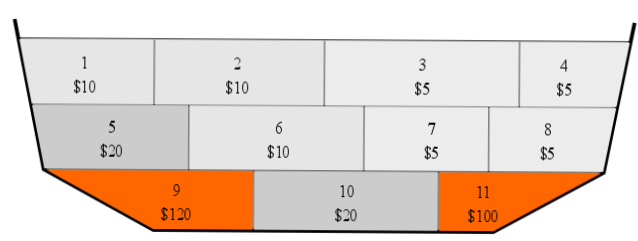
\includegraphics[width=12cm]{pit}
  \centering
  \caption{An example of an open-pit mine split into blocks. The blocks are numbered from 1-11 and are associated with values (dollar amounts). At the 
  bottom-left and bottom-right are two blocks of ore which provide profits of \textdollar120 and \textdollar100, respectively. All other blocks (shades of grey) 
  have negative dollar amounts.}
  \label{fig:pit}
\end{figure}

The aim is to extract the ore incurring the least costs and maximising the profit. We see that in order to get to the ore in the bottom-left, 
a total of \textdollar50 is incurred. Whereas, getting to the ore at the bottom-right requires \textdollar20. The total profit obtained from getting to block 9 is \textdollar70 and \textdollar80 for block 11 (assuming a single time period). Hence, if there were competing resources and a single time period, it is preferable to mine the sequence of blocks (3,4,7,8) to get to the ore in block 11.   

\subsection{Integer Programming Formulation of Open Pit Mining}\label{sec:formulations}

In this section we provide a MIP formulation of the PCPSP. Due to the complexity of the MIP, we also consider different algorithms to solve different aspects of the problem, e.g. the linear programming relaxation. Hence, we also consider alternative formulations that are useful in solving the problem. 

The PCPSP problem is to generate the maximum profit over the life of a mine taking into account the following restrictions: (a) each block is mined at most once, (b) predecessor blocks must be mined in the same period or earlier, (c) each block must be sent (possibly fractionally) to the destinations in  the period in which it is mined and (d) the resource limits consumed in sending blocks to their destinations must not satisfied.

The PCPSP problem\footnote{In this paper we use the benchmark data sets available in ``Minelib: A library of open-pit mining problems''~\citep{espinoza_minelib:_2012}.} consists of the following sets and parameters:
\begin{enumerate}
\item[$B$] The set of blocks (up to about 100,000 in the data sets we are
  interested in).
\item[$T$] the set of time periods (typically 20 or 30 years).
\item[$D$] the set of destinations. In the data there are normally just
  $|D|=2$, representing whether the  a block is discarded ($d=0$) or processed
  and sold ($d=1$).
\item[$R$] the set of resources (typically just 2, one for mining blocks and
  the other for processing of blocks).
\item[$\mathcal{P}$] the set of precedences. We write $a\rightarrow b$ if
  $(a,b)\in \mathcal{P}$ to mean block $a$ has to be mined before (or in the
  same period as) block $b$.
\item[$p_{bdt}$] the profit for sending block $b$ to destination in $d$ in
  time $t$ (can be negative if mining the block results in a net loss). For the
  MineLib data this is simply $\frac{p_{bd}}{(1+\alpha)^t}$ for
  some base cost $p_{bd}$ and $\alpha$ is a discount value that is typically a fraction between 0 and 1.
\item[$q_{bdr}$] the amount of resource $r$ required by block $b$ if sent to
  destination $d$. Note, for the datasets we are interested in this is either
  the tonnage of the block or zero if destination $d$ does not consume resource $r$.
\item[$\bar R_{rt}$] The amount of resource $r$ available in time period $t$
  (typically a constant that only depends on $r$ in our data sets).
\end{enumerate}


Given the above definitions of sets and parameters, we now describe the mathematical formulation. We introduce the following decision variables:
\begin{eqnarray*}
 \bar x_{bt} & = & \left \{ \begin{array}{ll}
                         1 & \hbox{if the  block has been removed by the end of period } t\\
                         0 & \hbox{otherwise}
                        \end{array} \right . \\
 y_{bdt} & \in & [0, 1] \hbox{ is the fraction of block } b \hbox{ sent to destination } d \hbox{ in period } t. 
\end{eqnarray*}
Using this notation we can write the problem formulation as:

\begin{alignat}{3}   %% number of &'s = 2 * cols - 1
  \noalign{\noindent\bf Problem PCPSP}
  %% alignment is right, left, right, left, ....
  &&\max\quad&\sum_{b\in B}\sum_{d\in D}\sum_{t\in T} p_{bdt}\,y_{bdt}   & \label{eq:obj} \\
  \text{s.t.} && \bx_{bt} &\,\leq\, \bx_{at}&&\forall\ (a,b)\in\mathcal{P},\ t\in T  \label{eq:prec}\\ 
  && \bx_{bt} &\,\leq\, \bx_{b,t+1} && \forall\ b\in B,\ t\in T \label{eq:once}\\
  &&\sum_{d\in D} y_{bdt} & \,=\, \bx_{bt}-\bx_{b,t-1}&&\forall\ b\in B,\ t\in T \label{eq:ydef}\\
  &&\sum_{b\in B}\sum_{d\in D} q_{bdr}\,y_{bdt}&\,\leq\, \bar R_{rt}&&\forall\
  r\in R,\ t\in T\label{eq:resource}\\
  &&\bx_{bt}\in\{0,1\},\ \ y_{bdt}&\,\geq\,0&&\forall\ b\in B,\ d\in D,\ t\in T \label{eq:vars}
\end{alignat}
Constraints \eqref{eq:prec} ensure that blocks are mined according to the precedence relations. 
The fact that a block cannot be mined more than once is represented by the constraints \eqref{eq:once}.
Constraints \eqref{eq:ydef} ensure that if a block is extracted then it must be sent to one or more destinations. 
Resource utilization requirements are presented by the constraints \eqref{eq:resource}.
For technical correctness note that in \eqref{eq:ydef} for the first time
period no previous $\bx$ is to be subtracted. 

The MIP formulation is equivalent to the formulation presented in MineLib, but the variable $\bx_{bt}$ has different meaning in the MineLib documentation, i.e., $x_{bt} = 1$ if block $b$ is mined at time-point $t$. The PCPSP problem can also be modelled with an aggregation formulation, which can be used to efficiently obtain the LP relaxation (details in Section~\ref{sec:MC}). Alternative network flow and aggregation based formulations are detailed in \ref{sec:network_flow}, \ref{sec:incremental} and \ref{sec:agg}.


\section{Application of Merge Search to the PCPSP}
In applying Merge Search to the problem in this paper we implement it as
follows. Firstly, the Merge Search method is used recursively as a
neighbourhood search mechanism. When used to generate neighbourhood solutions,
we simply split the binary variables $x$ into those that are zero and those
that are one in the current solution. For the continuous variables, a large
number of different fractional solutions are possible, but in practice
solutions tend to only have a very small number of different fractional
values as observed in the discussion of the Bienstock-Zuckerberg
approach (see Section~\ref{sec:bienstock}).

Our implementation uses a distributed computing approach with neighbourhood
search being carried out in different processes, each of which maintains its own population of solutions. The best solution found so
far is shared amongst processes in an asynchronous manner allowing each
process to carry out the merge operation of Step~\ref{step:merge}.

The merge step solves an aggregated version of the PCPSP.  The starting point 
for this merge step is a slight variant of the MIP formulation (described in detail in 
\ref{sec:incremental}) which only has one variable $\bar y_{bdt}$ for each (block, 
destination, time) triplet, rather than separate $\bar x$ and $y$ variables. We then 
define a partition as per Steps~\ref{step:P} and \ref{step:RandSplit} of 
Algorithm~\ref{alg:MS} by:
%\redsout{Bienstock-Zuckerberg formulation \eqref{eq:BZ:obj}-\eqref{eq:BZ:bounds}} 
%\eqref{eq:yobj}- \eqref{eq:yvars}. 
% Here we \emph{aggregate} variables to produce a much smaller set of variables that still includes all of the solutions that we started with, as well 
% as potentially more profitable combinations. 
%  The aggregations are defined in terms of a partition of the set of (block-time-destination) triplets that define our 
%
% Consider the following method of partitioning the set of (block-time-destination) triplets that define the $\bar y$ variables in the full formulation:
\begin{enumerate}
\item Start with all of the (block, destination, time) triplets in one large set,
\item Split out all triplets that have been fixed to zero or to one by preprocessing  into two separate sets based on their fixed values,
\item For any heuristic solution $\bar{\bm y}$, split sets in the partition so that all elements have the same value in $\bar{\bm y}$,
\item Split the partition further in a randomised manner up to a prescribed maximum number of sets.
\end{enumerate}
Based on such a partition, we now set up a variant of the formulation \eqref{eq:yobj}--\eqref{eq:yvars}
%\eqref{eq:BZ:obj}-\eqref{eq:BZ:bounds} 
in which there are only variables $\bar y_S$ for any 
set of triplets $S$ in the partition. This formulation really only has two types of constraints: precedence constraints $\bar y_S \le \bar y_P$ for two different 
partition sets $S,P$ where at least one pair of triplets are constrained in this way; and resource constraints that are aggregated versions 
of \eqref{eq:yresource} (see \ref{sec:agg} for details).
%\eqref{eqn:BZ:R}, \eqref{eqn:BZ:R2}. 
As noted above, any feasible solution used as input to the splitting process will be feasible for the simplified problem 
generated in this way. In addition, the optimisation searches over the space of combinations of solutions allowing multiple improvements to the previously 
best known solution to be merged into a single, even better solution.

The randomised additional splitting (Step~\ref{step:RandSplit} of
Algorithm~\ref{alg:MS}) generates an additional expanded neighbourhood of the starting solutions in which to search. In order to ensure that this 
neighbourhood has a reasonable chance of containing improving solutions, this additional partitioning is guided by the global best solution as follows:
\begin{enumerate}
\item Sets of triplets that are split out of a partition always form ``cones'' - that is, they are defined in terms of a (block, destination, time) triplet 
plus all of the predecessors (or all of the successors) of this triplet that are part of the same set in the current partition.
\item If the current best solution has a $\bar y_{b,t,d}=1$ then all of the successors are considered (as the neighbourhood move being contemplated is setting 
this variable and its successors to zero). Conversely if $\bar y_{b,t,d}=0$ we consider the predecessor cone.
\item A similar number of cones are generated in both directions, to maximise the probability that some combination of these can be swapped.
\end{enumerate}
Note that these restrictions on the types of random splits that are being considered are simply a way of ensuring that we have meaningful splits with a reasonable chance of improving the solution. For example if we carried out a split of some set $P\in\cal P$ into $P_1$ and $P_2$ in such a way that both a predecessor of some triplet in $P_1$ and a successor of some triplet in $P_1$ is in $P_2$ then the precedence constraints would enforce that $\bar y_{P_1}\ge \bar y_{P_2}$ and $\bar y_{P_1} \le \bar y_{P_2}$ (i.e. the two aggregated variables must take on the same value).  

In our implementation we used a
``recursive'' Merge Search method in which the neighbourhood search,
implemented in Step~\ref{step:nbhd}, is simply another Merge Search with
$m=0$ (i.e. relying purely on random splitting to generate a neighbouring
solution). This clearly results in a method that is purely an ascent approach.
However Lemma~\ref{thm:optimal} guarantees that it is at least theoretically possible to find an optimal solution. 
Furthermore, given the large instance size even a simple hill-climbing scheme would require a long time to reach a local optimum. The empirical evidence indicates that
it is not necessary to include any more sophisticated diversification methods in order to obtain good solutions. 

\subsection{Merge Search Example}
\begin{figure}[hb!]
  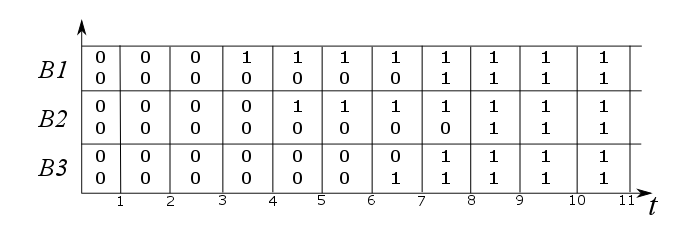
\includegraphics[width=14cm]{OPBS-MS-orig.png}
  \centering
  \caption{A problem with 3 blocks an two solutions. The mining time of each block varies depending on the solution; for example, Block 1 is mined at time-point 3 in the first solution whereas it is mined at time-point 7 in the second solution.}
  \label{fig:MSorig}
\end{figure}

To make our new algorithm easier to understand, we provide a simple example of how Merge Search can be applied to open pit mining. Figure~\ref{fig:MSorig} shows such an example of two solutions and the time-points when the three blocks (B1, B2 and B3) are mined. Given these two solutions, the solution space for the MILP is split into four sets (Figure~\ref{fig:MS1}). The white region consists of variables which were 0 in both solutions; light grey, where the first solution is 1 and the second is 0; dark grey, where first solution is 0 and second is 1;and black, where variables from both solutions are 1. When solving the corresponding MILP, all variables in each set are aggregated and required to take on the same value. For example, the variables in light grey region should either be all 0s or all 1s and similarly for the remaining sets. 

\begin{figure}[h!]
  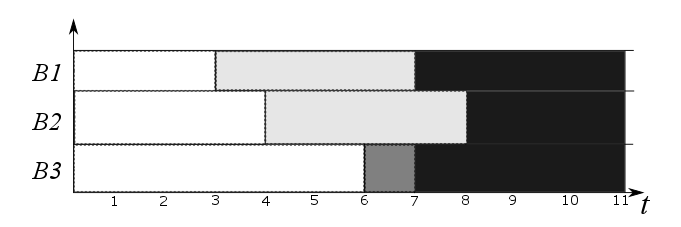
\includegraphics[width=14cm]{OPBS-MS.png}
  \centering
  \caption{The sets generated from the solutions in Figure~\ref{fig:MSorig}. The white region corresponds to both solutions having all variables 0 and the black region is one where all variables are 1. The grey areas are where the variables take on different values in both solutions; light grey is where the first solution is 1 and the second solution is 0; dark grey is the opposite, i.e., the first solution takes on value 0 and the second solution 1. }
  \label{fig:MS1}
\end{figure}

The fours sets in Figure~\ref{fig:MS1} can be too small to generate new and potentially improving solutions. Hence, we apply random splitting to the regions. An example of this can be seen in Figure~\ref{fig:MS2}. The light grey area is split into smaller sets allowing the possibility of generating a number of new solutions.\footnote{The dark grey area may not be split further as there are no integer time points between 6 and 7.}  Note that in this example if we split the variables so that there exist partitions $P$ and $Q$ with $(B1,4)\in P$ \& $(B1,7)\in P$ while the middle part $(B1,5)$ \& $(B1,6)$ are in $Q$, then the two partitions $P$ and $Q$ are forced to take on the same value by the requirement that a block that has been mined stays mined ($\bar y_{b,d,t+1}\ge y_{b,d,t}$ in constraint \eqref{eq:yincr}). In general, a larger number of sets allow more possibilities, leading to improved diversity. In the limit, splitting into sufficiently many subsets makes each $P$ a singleton, so that the problem to be solved in the merge step is just the original MIP.

\begin{figure}[h!]
  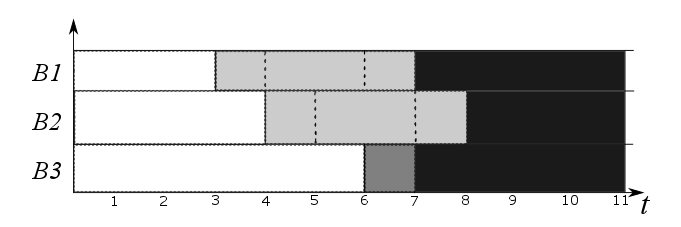
\includegraphics[width=14cm]{OPBS-MS2}
  \centering
  \caption{The sets generated from the solutions in Figure~\ref{fig:MSorig} and the sets are the same as that of Figure~\ref{fig:MS1}. The set in the light grey region is split into additional sets along the dotted lines. }
  \label{fig:MS2}
\end{figure}

\section{Efficient Implementation of Merge Search and a Branch \& Bound Method} \label{sec:meth}
As we are solving a large integer linear program it is advantageous to solve the LP relaxation of the problem. This is used in several ways: (a) to provide a relaxed bound (quality guarantee), (b) for a rounding heuristic to generate a promising initial solution, and (c) as a basis for a simple branch and bound method that could in principle produce optimal solutions. 
In this section, we outline some of the methods that have been used. While these are less novel than Merge Search itself, they make a significant difference to the empirical performance reported in this paper. Furthermore, some of these small algorithmic improvements have not to the best of our knowledge been described briefly in the literature. Hence, we describe these briefly for completeness.  Specifically, the methods discussed are:
\begin{itemize}
\item Preprocessing: in order to make the solvers efficient, preprocessing is used to substantially reduce the problem size.
\item Max closure solver: this algorithm is often used as a part of the other methods and we hence provide the details of its implementation, including the best approach for solving it.   
\item LP relaxation: due to large run-time requirements of obtaining the LP relaxation, we implement the more efficient Bienstock $\&$ Zuckerberg method \citep{zuckerberg2010}. It uses the max closure solver as its basis. Through this method, we obtain both relaxed bounds, and via a rounding heuristic, an initial heuristic solution. 
\item Branch \& Bound: using the LP relaxation as a basis, we implement a Branch \& Bound method.
\item Distributed implementation: Allowing multiple CPUs (computers) to solve these challenging problems was a significant factor in motivating the development of Merge Search. We discuss how this has been implemented for our computational experiments.
\end{itemize}

\subsection{Preprocessing}\label{sec:preprocess}
In order to reduce the instance size as much as possible, some preprocessing is performed to eliminate variables that can never appear in the optimal solution. The preprocessing is carried out on all instances before any other solvers are used.

The first preprocessing method is to solve the {\it ultimate pit problem} (UPIT); a mine planning problem with no resource constraints. This computes all
blocks that would be considered if everything could be mined in the first period, and
with no restriction on the number of blocks that can be processed. Any blocks that
are not included in this unrestricted version would never be profitable to be
mined in the PCPSP and are thus removed.

Secondly, the number of possible destinations for some of the blocks can be
reduced. Essentially, if a block contains little valuable ore,
processing it will be both less profitable and more resource intensive to
process the block than to discard it. In this case, the number of destinations
can be reduced, again simplifying the problem and eliminating a continuous
variable (for the fraction of the block to be processed).

The final preprocessing method considers, for each block, the cone of
predecessors. We can then compute the minimum amount of resources required to
mine both the block and all of its predecessors. From this we can calculate the
earliest possible period when the block is to be mined. For some of the deeper
blocks this can significantly restrict the number of time periods that have to
be considered. 

\subsection{Maximum Closure Solver}\label{sec:MC}
As a sub-algorithm in many of the other methods proposed, it is necessary to solve the {\em Maximum Closure Problem} which is equivalent to the UPIT problem. This is defined as 
\begin{eqnarray}
 \max && \sum_{v\in V} p_v x_v  \label{eq:MC:obj}\\
 \text{Subject to}&& x_v \ge x_w \qquad\forall\ (v,w)\in A\\
 &&x_v\in \{0,1\} \qquad\forall\ v\in V\label{eq:MC:bounds}
\end{eqnarray}
Where $V$ is a set of vertices (in our case these correspond to block, time, destination triplets) and $A$ a set of arcs. For the problem we are 
interested in, these are based on the precedence restrictions and the requirement that once a block is mined, it stays mined. 

As has been noted by \cite{dorit_s._hochbaum_performance_2000}, the dual of the maximum closure problem can be modelled as a network flow or maximum flow
problem allowing it to be solved comparatively easily. See \ref{sec:network_flow} for details of this transformation. It should be noted
though that the instances are \emph{very} large with many millions of arcs for
the largest data sets. We tested three different algorithms:
\begin{description}
  \item[\quad P:] The "Push-Relabel" method for maximum flow problems. This is the method recommended in the literature (see \cite{dorit_s._hochbaum_performance_2000}). 
  We used a standard implementation from the Boost Graph Library\footnote{See \url{http://www.boost.org/doc/libs/1_63_0/libs/graph/doc/push_relabel_max_flow.html}} 
  with a theoretical complexity of $O(n^3)$, rather than a custom implementation as discussed in the literature. This method performed worst in our 
  experiments.
  \item[\quad N:] The Network simplex algorithm as implemented in the commercial CPLEX library. This is expected to be a slightly less efficient than the maximum 
  flow algorithms but has the advantage that re-solving with changed costs is sometimes faster than solving the problem the first time.
  \item[\quad B:] The Boykov-Kolmogorov Algorithm~\citep{boykov_experimental_2001}, which is related to augmenting paths, but improves efficiency by maintaining two 
  trees that are grown from the source and sink nodes. It has a theoretical complexity of $O(mn^2 |C|)$ though it has been found to perform much better 
  in practice. The implementation from the Boost Graph Library\footnote{See \url{http://www.boost.org/doc/libs/1_63_0/libs/graph/doc/boykov_kolmogorov_max_flow.
html} } has been used. 
\end{description}
Table~\ref{tab:MC} below provides  brief experimental results that indicate the relative effectiveness of these methods for solving 
instances of max closure problems encountered in this work. Each method was run repeatedly during the solution of the LP relaxation using the algorithm 
described in Section~\ref{sec:bienstock} (approximately 30 times each). See Table~\ref{tab:instances} for more information about the instances.

% \begin{table}[!htb]
% \centering
% \caption{CPU time (seconds) of 3 maximum closure methods with preprocessing of 30 solves (with different objective values) each on 3 data sets.}
% \label{tab:MC}
% \begin{tabular}{lccrrrrrr}
% \toprule
% Instance	&&	Method	&&	fastest	&&	average	&&	slowest \\
% \cmidrule{1-1}\cmidrule{3-3}\cmidrule{5-5}\cmidrule{7-7}\cmidrule{9-9}
% Zuck\_small && P &&   8.47 &&  10.43 &&  14.14\\
% Zuck\_small && N &&   0.22 &&   6.60 &&  37.44\\
% Zuck\_small && B &&   1.22 &&   4.10 &&   8.73\\
% KD         && P &&   4.30 &&   7.97 &&  10.19\\
% KD         && N &&   0.15 &&   5.78 &&  15.33\\
% KD         && B &&   0.56 &&   5.17 &&  13.29\\
% Zuck\_medium&& P &&  64.27 &&  86.70 && 122.04\\
% Zuck\_medium&& N &&   1.14 &&  70.99 && 334.31\\
% Zuck\_medium&& B &&  17.61 &&  57.50 && 150.20\\
% \bottomrule
% \end{tabular}
% \end{table}

Based on these results we note that the method recommended in the literature is the slowest. We would recommend method {\bf B} as having the best performance on average. However, given the smaller memory footprint (observed anecdotally but not measured systematically) and the occasionally faster run times of the network flow method (N), this could also be considered. For the implementation of these methods it should be noted that:
\begin{description}
\item[Numerical Stability:] Due to the large range of floating point numbers
  involved and the size of the instances, numerical stability is an issue. The
  use of scaling helps to alleviate this to some degree. Nevertheless, for the
  largest instances, the solution of the maximum closure problem may only be an
  approximation. This is particularly problematic for Lagrangian or dual type
  methods, where small changes in cost are used to try to push the solution
  towards feasibility (not described here). Given the large magnitude of some
  of the costs involved, small changes to the costs can get lost based on the
  numerical accuracy limits of the computer.
\item[Preprocessing:] The graph structure arising from the
  Bienstock-Zuckerberg formulation contains many chains of nodes (connected
  sets of nodes with indegree and outdegree at most 1). These particularly
  occur where there are multiple destinations for the same block. For any
  such chain of nodes there are three possible options:
  \begin{enumerate}
  \item All of the nodes are included, if the end of the
    chain is in the closure;
  \item All of them are excluded, if the start is not in the
    closure; or
  \item The chain an be broken into two parts $A$ and $B$, with part $A$ included in
    the closure and B excluded. The optimal division of the chain into parts $A$
    and $B$ can be precomputed independently for each chain.
  \end{enumerate}
  Hence, we can modify the problem to remove the chain and replace it with  a
  single arc from the node at the start of the chain to the node at the end.
  The value of the start node is increased by the total value of nodes in $A$
  ($\sum_{v\in A} p_v$),  while the value of nodes in $B$ is added to the node
  at the end of the chain. All intermediate nodes can be removed.
  This preprocessing step has a significant positive
  effect on the efficiency with which the max closure subproblems can be
  solved. 
\end{description}
During the solution process we are interested branching on $x_v$ variables or fixing some of these based on preprocessing the overall problem. 
However, all of the solution approaches solve the linear programming dual of the formulation \eqref{eq:MC:obj}--\eqref{eq:MC:bounds}. Thus it is not possible 
to fix variables directly (fixed variables correspond to constraints in the dual problem). Again, we resort to a preprocessing step that removes variables in 
the maximum closure problem before passing it to the solver. 

\subsection{Solving the LP relaxation}\label{sec:bienstock}

The LP relaxation of the PCPSP is solved using the Bienstock--Zuckerberg algorithm~\citep{zuckerberg2010} has been developed to solve the LP relaxation of 
large scale precedence constrained production scheduling problems. This is a type of decomposition approach with some similarity to column generation. It iterates between solving a master problem, that is essentially the LP relaxation of the merge problem (that is it is a reduced problem defined by a partition of the variables) and a subproblem that is equivalent to the Lagrangian relaxation obtained by dualizing the resource constraints \eqref{eq:yresource}. The problem that has to be solved for a given Lagrange multiplier $\mu\ge 0$, is
\begin{alignat}{3}
  \noalign{\noindent\bf Problem $L(\mu)$}
  %% alignment is right, left, right, left, ....
  &&\max\quad&\sum_{b\in B}\sum_{d\in D}\sum_{t\in T} \big(\bar p_{bdt}&&-\sum_{r\in R}q_{bdr}\mu_{rt}-q_{bd'r}\mu_{rt'}|_{(d',t')\rightarrow(d,t)}\big)\,\bar y_{bdt}    \label{eq:Lobj}\\
  \text{s.t.} && \by_{b0t} &\,\leq\, \by_{a0t}&&\forall\ (a,b)\in\mathcal{P},\ t\in T  \label{eq:Lprec}\\ 
  && \by_{bd't'} &\,\leq\, \by_{bdt} && \forall\ b\in B,\ d\in D,\ t\in T,
  \text{ if }(d,t)\rightarrow(d',t') \label{eq:Lincr}\\
  % &&\sum_{b\in B}\sum_{d\in D} q_{bdr}\,\left(
  %   \by_{bdt}-\by_{bd't'}|_{(d,t)\rightarrow(d',t')}
  % \right)&\,\leq\, \bar R_{rt}&&\forall\  r\in R,\ t\in T\label{eq:yresource}\\
   &&0\leq \by_{bdt}&\,\leq\, 1
  &&\forall\ b\in B,\ d\in D,\ t\in T \label{eq:Lvars}
\end{alignat}
This problem is exactly the maximum closure problem.
In the master problem a partition $\cal S$ of the variables is used to solve the LP relaxation of PCPSP$(\mathcal{S})$, that is the aggregated problem also used during the merge step. The dual values of the resource constraints \eqref{eq:Sresource} are used to update the Lagrange multipliers $\mu$. The subproblem solution $\bar y^*$ is then used to refine the partition $\mathcal{S}$  by splitting any sets that are only partly in the optimal closure defined by $\bar y^*$. The 
algorithm is presented in Algorithm~\ref{alg:bz}. Note that this algorithm iterates between finding valid upper (relaxed) bounds via Lagrangian relaxation 
and valid LP lower bounds (feasible fractional solutions $y^k$) by solving aggregated LPs. The master problem LPs simply require that any pair of 
variables (corresponding to block-destination-time triplets) that have had the same solution value in each of the 
Lagrangian iterations so far, must also take the same value in the LP (See Step~\ref{step:aggregate} of Algorithm~\ref{alg:bz}).  For more 
details see~\cite{zuckerberg2010}. 
\begin{algorithm}[h!]
\def\IFstop#1{\State \algorithmicif\ #1 \algorithmicthen\ STOP}
\caption{{\sf Bienstock--Zuckerberg Algorithm}} \label{alg:bz}
\begin{algorithmic}[1]
\State {\bf Initialize:} $\mu^{0}=0$, $\mathcal{S}^{0} = \lbrace \mathcal{N}\rbrace$ ($\mathcal{N}=B\times D\times T$), $r^0=0$, $z^{0} = - \infty$, $k=1$.
\For{Iteration $k=1,2,\ldots$}
  \State {\bf Use Max--Closure Algorithm} to obtain $\bar y^k$ to $L(\mu ^{k-1})$ 
  \State {\bf Let:} $I(\bar y^k) = \{ n \in \mathcal{N} \mid \bar y^k_n = 1 \}$ and $O(\bar y^k) = \lbrace n \in \mathcal{N} \mid y^k_n = 0 \rbrace$
  \State {\bf Let:} $\mathcal{S}^k=\left\{S\cap I(\bar y^k) \mid S\in\mathcal{S}^{k-1}\ \&\ S\cap I(\bar y^k)\ne\emptyset\right\} \cup \left\{S\cap O(\bar y^k) \mid S\in\mathcal{S}^{k-1}\ \&\  S\cap O(\bar y^k)\ne\emptyset\right\}$
  \IFstop{$\mathcal{S}^k=\mathcal{S}^{k-1}$}
  \Comment{i.e. finish if the partition is unchanged.} 
  \State Solve the LP relaxation of PCPSP$(\mathcal{S}^k)$ 
  to get optimal solution $y^k$. \Comment{See \eqref{eq:Sobj}--\eqref{eq:Svars}} \label{step:aggregate}
  \State \algorithmiccomment {Note that $y^k_{b,d,t}=y^k_{b',d',t'}$ whenever $(b,d,t)$ \& $(b',d',t')$ are in the same set $S\in\mathcal{S}^k$ }
  \State {\bf Let} $\mu^k$ be the optimal dual values of the resource constraints \eqref{eq:Sresource}.
  \IFstop{$\mu^k = \mu^{k-1}$} 
 \EndFor
\end{algorithmic}
\end{algorithm}
\subsubsection{Rounding Heuristic}\label{sec:round}
The LP relaxation of the PCPSP provides valuable information regarding the `preference' of when the blocks should be mined. Here, a greedy approach is implemented to construct an integer solution from a fractional solution to the LP relaxation. Each time, the block with highest preference is selected from among the available blocks. 
The preference relation is defined using lexicographical order of 
\begin{enumerate}
\item Accessibility -- number of remaining predecessors
\item Accumulated weight -- cumulative sum of fractional values
\item Start period in fractional solution
\item Precedence relations between blocks
\item Maximum marginal profit per unit of resource 
\end{enumerate}
In this greedy approach, we consider periods one by one, starting from the
first period, until all blocks with positive marginal profits are scheduled; or we have reached the end of the planning period. In each period, blocks are added until
resources are fully utilized. For each selected block, the destinations are
determined using a greedy approach based on marginal profits (as large as possible a fraction of the block sent to the destination with the highest marginal
profit). Once a schedule is obtained, the distribution of the blocks in each
period is refined using an LP approach to improve the total profit, if possible.

The rounding heuristic on its own does not perform very well. However, it runs reasonably quickly once the LP solution has been obtained and allows us to produce both a lower bound and an upper bound based on the Bienstock-Zuckerberg algorithm. 

\subsection{Branch \& Bound}\label{sec:BB}
The LP solution obtained using the Bienstock-Zuckerberg algorithm can be used
in a branch and bound method to search for an optimal integer solution. A
depth-first branch and bound method has been implemented for comparison
purposes, since none of the MILP formulations presented above can be used
directly with a MILP solver (the instances are far too large). While theoretically this would allow the problems to be solved exactly, in practice this cannot be expected within a reasonable time limit. No attempt has been made to explore alternative branching strategies, and we leave this aspect to future work.

\subsection{Parallel and Distributed Computing}\label{sec:parallelms}

Two different types of parallelisation were considered in this paper. Firstly, a multi-core shared memory architecture via OpenMP~\citep{openmp} is used by 
any MIP based implementation, either by Gurobi or CPLEX. Either of these solvers will always use as many cores as possible from those that are made available to them.

Secondly, we use an MPI distributed framework (\cite{Gropp:1994}). The implementation for this study is not a traditional master/slave framework. Rather, each node 
consists of a master and a slave thread. The master thread ensures the communication requests are processed in a timely manner, while the slave does most 
of the computational work.  

Figure~\ref{fig:mpi-comm} demonstrates the architecture.  Both threads maintain copies of the solution information, while the master solution (within grey 
region of a node) is the only one that is broadcast (grey links). It is also the only one updated with solution information from other nodes (blue links). 
Periodically, the solution information from the slave is updated to the master's solution (links within nodes). Conversely, when there is a new solution 
which is an improvement over the master's solution, the master's solution is updated and broadcast to the other nodes.  

% DT: need to produce a different figure (can be similar but the current one is not appropriate) for this paper
 \begin{figure}[htbp]
   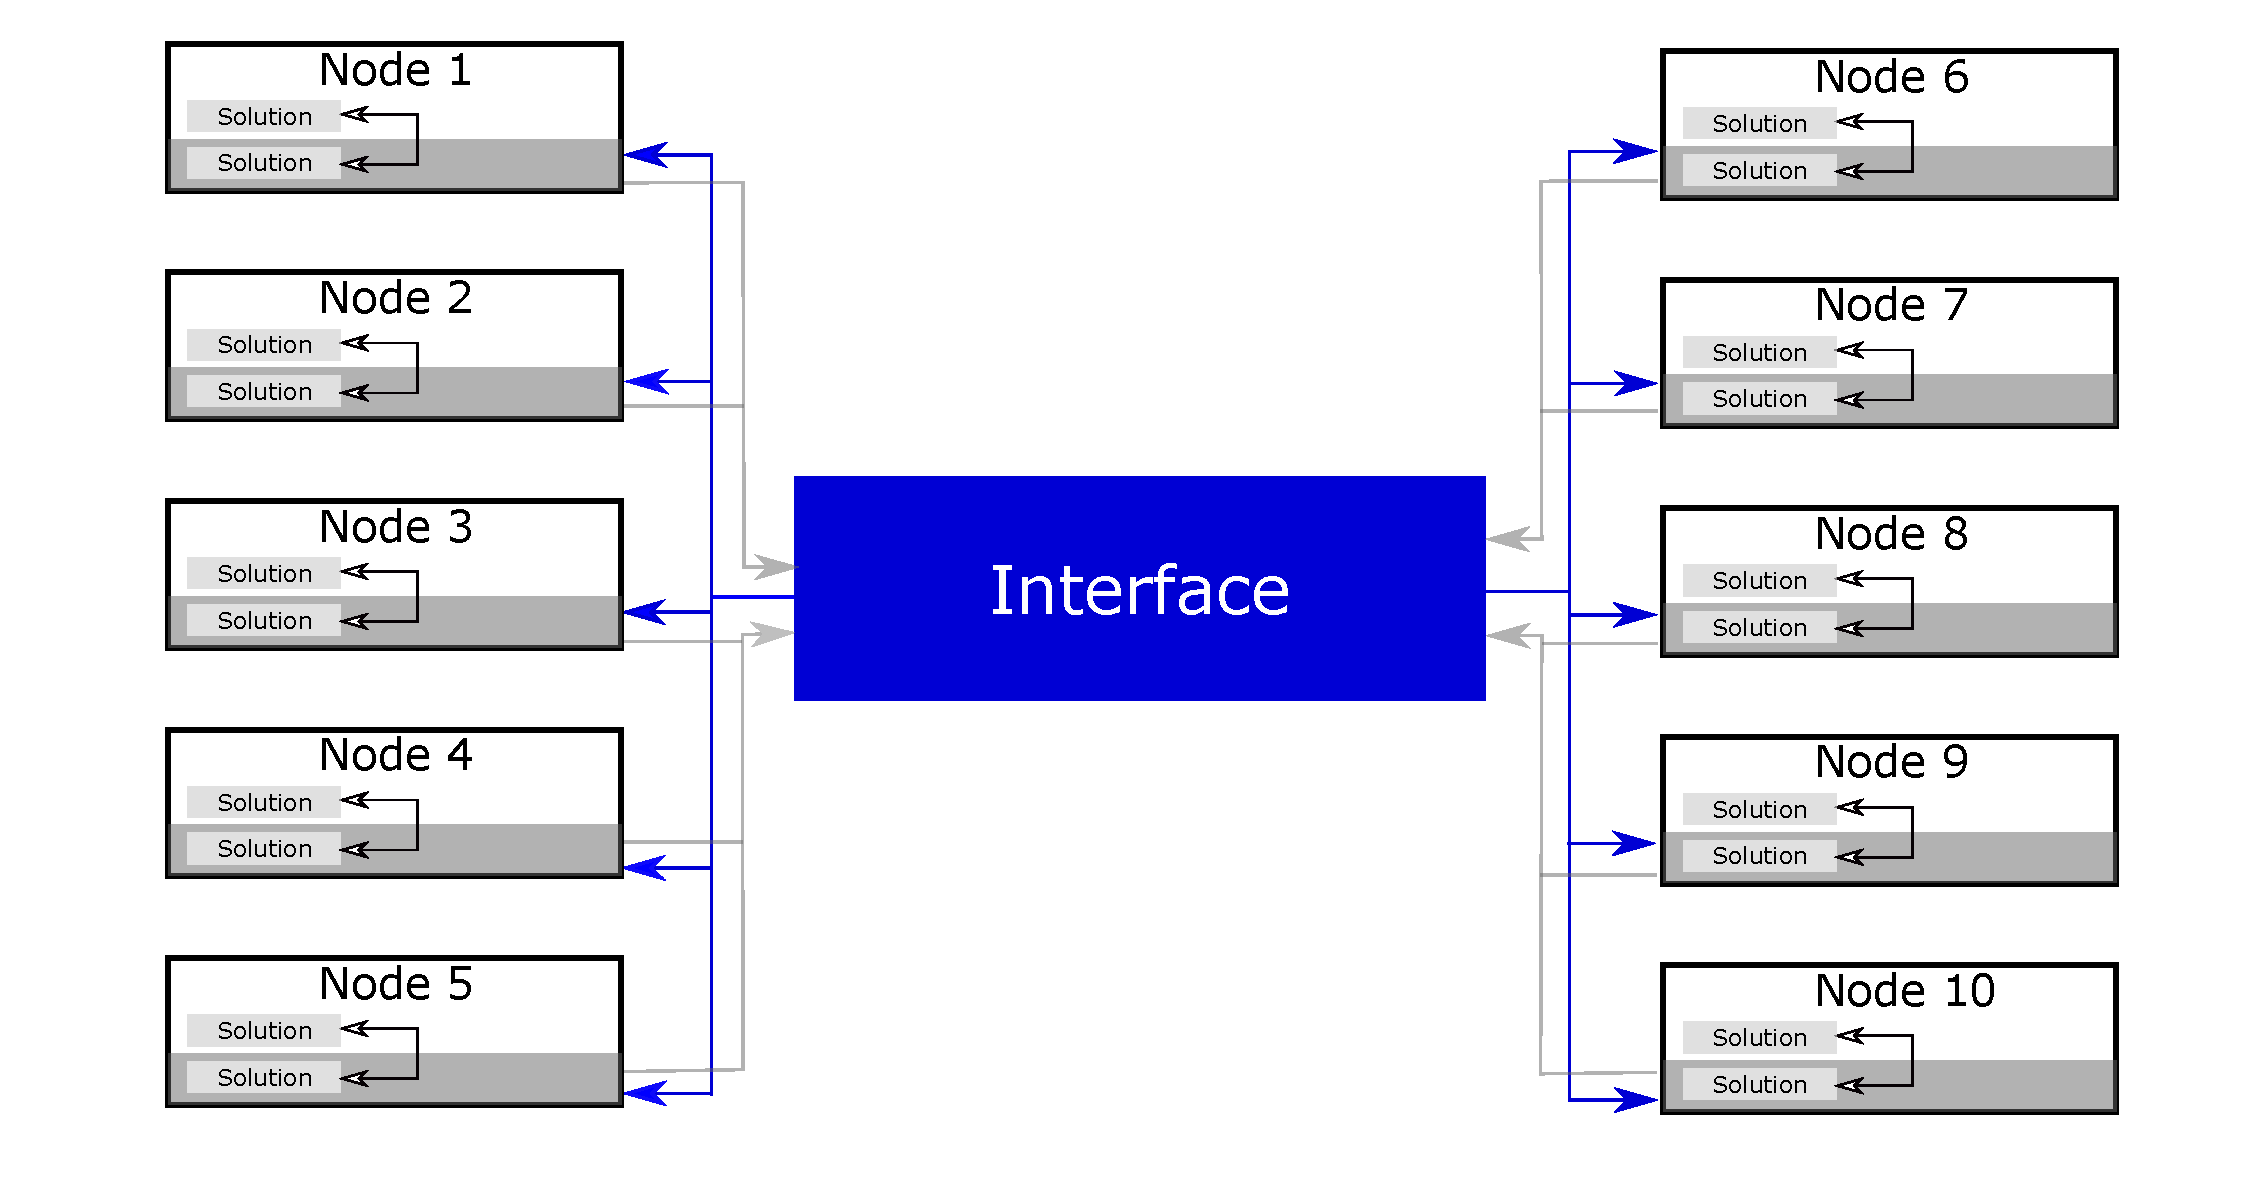
\includegraphics[width=15cm]{MPI-comm.pdf}
   \centering
   \caption{Communication in the MPI framework with 10 nodes. Each node consists of at least two threads, a master (grey) and a slave (white). Via the 
   interface, solutions are broadcast from each node to every other node.}
   \label{fig:mpi-comm}
 \end{figure}

\section{Computational Experiments \& Results} \label{sec:expts_res}
All code was implemented in C++ with GCC-4.8.0. For the parallel implementations, Intel and GCC compilers were tested and we settled on GCC. For CPLEX or 
Gurobi, a maximum of 6 threads were made available as we found no improved performance with a larger number of threads. In the case of MPI runs, the number of 
nodes used are specified with the results. 

%% The parallel experiments were run on Monarch
%% (\url{https://confluence.apps.monash.edu/display/monarch/MonARCH+Home}). This
The parallel experiments were run on a cluster comprising 35 nodes of which we
made use of 12 of these nodes which had up to 228 GB resident
memory.\footnote{Each algorithm requires at least 10 GB memory.}  To solve the MIPs, Gurobi 6.5.1\footnote{\url{http://www.gurobi.com/} } and CPLEX 12.6.3\footnote{\url{https://www-01.ibm.com/software/commerce/optimization/cplex-optimizer/} } were used.

\subsection{Problem Instances}
\begin{table}[!htbp]
\centering
\caption{Selected problem instances from MineLib} 
\label{tab:instances}
\begin{tabular}{lrrrrrrrr}
\toprule
Instance && No. Blocks && No. Precs && No. Periods\\
\cmidrule{1-1}\cmidrule{3-3}\cmidrule{5-5}\cmidrule{7-7}
Newman1 && 1,060 && 3,922 && 6  \\
Zuck$\_$small && 9,200 && 145,640 &&20  \\
Zuck$\_$medium && 29,277 && 1,271,207 && 15  \\
Zuck$\_$large && 96,821 && 1,053,105 && 30  \\
Kd && 14,153 && 219,778 && 12  \\
Marvin && 53,271 && 650,631 && 20  \\
Sm2 && 99,014 && 96,642 && 30  \\
\bottomrule
\end{tabular}
\end{table}

As discussed earlier, the problem instances were taken from MineLib (\url{mansci-web.uai.cl/minelib/}). The instances and their characteristics can be seen in Table~\ref{tab:instances}. The Newman1 dataset can be solved to optimality with the full MIP model within 10 minutes. All the remaining instances are too large to even obtain the LP relaxation in reasonable time. Hence, the Bienstock \& Zuckerberg method has been used for this purpose. Note, we do not consider three problems instances from MineLib in this study: p4hd, w23 and mclaughlin. The first two include lower bounds on the resources constraints, for which the methods proposed here cannot easily deal with. The mclaughlin instance proves too large, which proves too memory intensive for the MS-based methods.  

\subsection{Computational Results}\label{sec:ser_res}
In the following discussion, we have two main comparisons. The first is the lower bound, produced by all the algorithms. Second, some of the algorithms produce upper bounds (e.g. Branch \& Bound), and we compare these to the results in Minelib. All the methods we compare are:
\begin{description}
\item[BZ:] Bienstock \& Zuckerberg. This solves the linear programming
  relaxation only and constructs a heuristic solution with the rounding
  heuristic described in Section~\ref{sec:round}. This is essentially a
  serial algorithm. It uses the maximum closure solver with the
  Boykov-Kolmogorov algorithm.
\item[MS:] Merge Search starts with the BZ algorithm and then applies the
  Merge Search Algorithm~\ref{alg:MS} on a single computer. We use $m=100$ and
  $K=10000$ 
\item[B\&B:] Branch \& Bound as described in Section~\ref{sec:BB}
\item[P-MS:] Parallel Merge Search runs the same MS method in multiple (12)
  processes and periodically merges the best solutions found across all of the
  distributed runs. 
\item[WS:] The results obtained in the ``Window Search'' method described in the study by \citet{Kenny:2017}.
\item[MineLib:] This refers to the best known results as published
  in~\cite{espinoza_minelib:_2012}.
\end{description}

The results are presented in Table~\ref{tab:results}, which includes all the algorithms being compared and also the results from Minelib. For the algorithms proposed in this study (BZ, MS, B\&B and P-MS), a maximum of five hours of wall-time was allowed. The reason for using this limit is that we are able to achieve as good if not better results in shorter run-times than previous studies ($\geq 10$ hours, e.g. the study by \citet{Kenny:2017}). In the case of P-MS, 12 nodes were allowed. The {\it Best LB} is the best lower bound achieved across all the algorithms including also the results from \citet{Kenny:2017} and MineLib. The gaps to the best upper bound are also provided (Gap $\%$  = $\frac{(UB*-LB) \times 100}{UB*}$, where UB* is the upper bound found by B$\&$B). Note, due to very high communication overheads, no solution could be obtained P-MS for $Newman1$.\footnote{Since $Newman1$ is relatively small (approx. 1000 blocks and 4000 precedences) and can be solved to optimality within 10 minutes by original MILP, there is no need for an efficient solution method. However, we still provide the results for this instance for the sake of completeness.} 

First, comparing lower bounds, we see that P-MS is consistently the best performing  algorithm (finds best solutions on 5 out of 7 problem instances). MS on its own is effective, also finding best solutions for two instances ($Zuck\_small$ and $Marvin$). This shows that the parallel implementation provides substantial benefit when problem instances start becoming large. For $Zuck\_medium$, the window search of \citet{Kenny:2017} performs best and for $Zuck\_large$ the result from MineLib is the best. In these two cases, the number of constraints proves to complex for the MS-based algorithms (or Branch \& Bound) as the short time limit proves too restrictive. Specifically, $Zuck\_large$ happens to be the instance with the largest number of edges in the time-expanded precedence graph and $Zuck\_medium$ consist of the largest number of precedences overall. 

A final point about the lower bounds is that, among the methods proposed in this study (BZ, MS, B\&B, P-MS), BZ performs best on $Zuck\_large$. This is due to the rounding heuristic, which proves to be effective when the problem sizes are too large for the  MS-based algorithms to cope with.

\begin{table}[!htbp]
\centering
\caption{Results for the serial and parallel runs for each algorithm with a time limit of 5 hours. The problems Zuck$\_$small, Zuck$\_$medium, and Zuck$\_$large are listed as small, 
medium and large, respectively. The best MineLib results are also provided for comparisons. The last row specifies the best lower bound (Best LB) found 
across all the algorithms, including the MineLib results. Gaps (Gap $\%$) to the upper bounds are also provided for each instance.}
\label{tab:results}
\scalebox{0.85}{
\begin{tabular}{llcccccccccccccc}
\toprule
\multicolumn{2}{l}{Algorithm}  && Newman1 && small && medium && large && Kd && Marvin && Sm2 \\
\cmidrule{1-2}\cmidrule{4-4}\cmidrule{6-6}\cmidrule{8-8}\cmidrule{10-10}\cmidrule{12-12}\cmidrule{14-14}\cmidrule{16-16}

BZ	&	LB	&	&	2.37E+07	&	&	7.21E+08	&	&	5.53E+08	&	&	5.08E+07	&	&	3.73E+08	&	&	7.29E+08	&	&	1.64E+09	\\
&	Gap $\%$	&&	2.07	&&	19.89	&&	26.07	&&	11.34	&&	8.80	&&	19.54	&&	0.61	\\
	& UB && {\bf 2.42E+07} && 9.05E+08 && {\bf 7.48E+08} && 	 5.79E+07 && 4.11E+08 && 9.12E+08 && 1.652E+09 \\
	
	%&	Gap 	&	&	2.15	&	&	19.51	&	&	19.76	&	&	11.35	&	&	8.48	&	&	19.07	&	&	0.40	\\

\midrule
MS	&	LB	&	&	{\bf 2.42E+07}	&	&	{\bf 8.95E+08}	&	&	 6.81E+08	&	&	4.69E+07	&	&	4.06E+08	&	&	{\bf 9.00E+08}	&	&	1.63E+09	\\
&	Gap $\%$	&&	{\bf 0.00}	&&	{\bf 0.56}	&&	8.96	&&	18.15	&&	0.73	&&	{\bf 0.66}	&&	1.21	\\

	%&	Gap 	&	&	0.00	&	&	0.00	&	&	1.24	&	&	18.23	&	&	0.22	&	&	0.00	&	&	1.28	\\
	
\midrule
B$\&$B	&	LB	&	&	2.42E+07	&	&	8.50E+08	&	&	6.38E+08	&	&	5.02E+07	&	&	1.82E+08	&	&	8.28E+08	&	&	1.65E+09	\\
&	Gap $\%$	&&	0.00	&&	5.56	&&	14.71	&&	12.39	&&	55.50	&&	8.61	&&	0.00	\\


	%&	Gap 	&	&	0.01	&	&	5.09	&	&	7.53	&	&	12.49	&	&	55.29	&	&	8.09	&	&	0.03	\\
	&	UB	&	&	{\bf 2.42E+07}	&	&	{\bf 9.00E+08}	&	&	{\bf 7.48E+08}	&	&	\bf 5.79E+07	&	&	{\bf 4.09E+08}	&	&	{\bf 9.06E+08}	&	&	{\bf 1.65E+09}	\\
\midrule
P-MS	&	LB	&&	- && {\bf 8.95E+08}	&&	7.12E+08	&&	4.06E+07	&&	{\bf 4.07E+08}	&&	{\bf 9.00E+08}	&&	{\bf 1.65E+09}	\\

&	Gap $\%$	&&		&&	{\bf 0.56}	&&	{\bf 4.81}	&&	29.14	&&	{\bf 0.49}	&&	{\bf 0.66}	&&	{\bf 0.00}	\\
	%&	Gap	&&	- && 0.11	&&	17.25	&&	29.16	&&	0.19	&&	0.61	&&	{\bf 0.00}	\\
	
	&	Nodes	&&	- && 12	&&	12	&&	12	&&	12	&&	12	&&	12	\\	
   \midrule
   
WS  & LB & & 2.41E+07 && 8.91E+08 && {\bf 7.28E+08} && 5.70E+07 && 4.02E+08 && 5.70E+07 && - \\
\midrule
MineLib	&	LB	&	&	2.37E+07	&	&	7.99E+08	&	&	6.76E+08	&	&	{\bf 5.73E+07}	&	&	4.07E+08	&	&	8.86E+08	&	&	{\bf 1.65E+09}	\\
&	Gap $\%$	&&	2.07	&&	11.22	&&	9.63	&&	0.00	&&	0.49	&&	2.21	&&	0.00	\\

	%&	Gap 	&	&	2.15	&	&	10.73	&	&	2.01	&	&	0.00	&	&	0.04	&	&	1.61	&	&	0.00	\\
    &	UB	&	&	2.45E+07	&	&	9.06E+08	&	&	7.51E+08	&	&	 5.79E+07	&	&	4.11E+08	&	&	9.12E+08	&	&	1.652E+09	\\
\midrule
Best LB	&		&	&	2.42E+07	&	&	8.95E+08	&	&	7.28E+08	&	&	5.73E+07	&	&	4.07E+08	&	&	9.00E+08	&	&	1.65E+09	\\
\bottomrule
\end{tabular}
}
\end{table}
%\comment[AE]{I'm somewhat perplexed that the LB of P-MS is much worse than that of BZ. Since we are running BZ initially surely we should get at least the same bound as that method (?). If that is not a typo then we should include at least a brief comment as to why this might be the case}

The second result of interest is regarding the upper bounds (comparing UB within BZ, B$\&$B and MineLib). The BZ algorithm provides upper bounds very close to the of the original LP upper bounds, which is expected as this is what the BZ method is designed to do. However, in the case of $Zuck\_medium$, the upper bound has been improved substantially, demonstrating the effectiveness of the preprocessing describe in Section~\ref{sec:preprocess}. The B$\&$B algorithm improves upon the upper bounds of BZ (except $Zuck\_medium$, where the upper bounds found are the same) but cannot close the gap to the best known solutions for most instances.
 
\subsubsection{Convergence of MS and P-MS}
We examine the convergence behaviour of MS and P-MS, the two best methods for obtaining lower bounds. For this purpose, we limit both algorithms to two hours of run-time. The results are presented in Figure~\ref{fig:con_summary}, for which we consider only the instances where MS and P-MS were most successful ($Zuck\_small$, \emph{Kd, Marvin} and \emph{Sm2}). The result is computed as follows. For each instance at each time point, the difference to the best solution at the end of the run is computed as $\frac{LB^*-LB}{LB^*}$. Then at each time point these values are averaged. Interestingly, initially, there is already a very large difference in favour of P-MS. This shows that a large amount of diversity leads to MS improving substantially, even for a single MILP solve. Overall, the parallel implementation with the assistance of the additional nodes allows the algorithm to converge more quickly to the best solution. Even though MS catches up at some time points, P-MS usually continues its improvement over the horizon. 

\begin{figure}[htbp]
  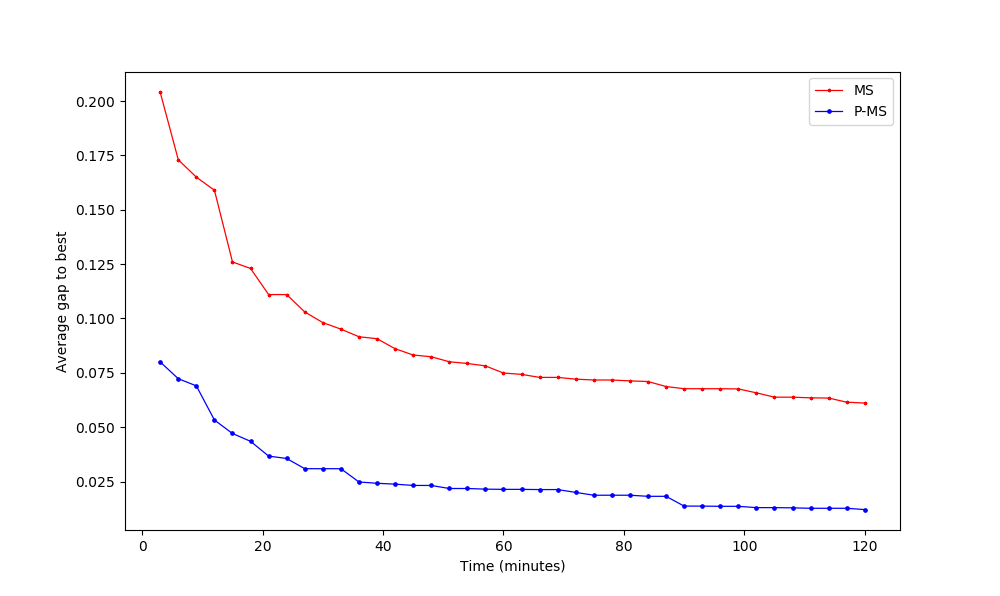
\includegraphics[width=15cm]{Convergence_summary}
  \centering
  \caption{Convergence of MS and P-MS for the smaller instances including Zuck$\_$small, Kd, Marvin and Sm2. The y-axis show the gap to the 
  best solutions found across all these instances.}
  \label{fig:con_summary}
\end{figure}

The next experiment aims to determine how P-MS converges with a differing number of nodes (processes run in parallel, not necessarily on different computers). The results are presented in Figure~\ref{fig:concores}. Compared to Figure~\ref{fig:con_summary}, this figure additionally includes $Zuck\_medium$ and we have run the algorithms for five hours. Like Figure~\ref{fig:con_summary}, the result is computed as the difference to the best solution at the end of the run $\frac{LB^*-LB}{LB^*}$. Again, initially there is a large difference depending on the number of cores. The only real stand-out at five minutes is the 12-core run. After about 35 minutes, we see increasing improvements with an increasing number of cores. This is not surprising since increasing the cores leads to improved diversity, which in turn leads to identifying more promising areas of the search space.

\begin{figure}[htbp]
  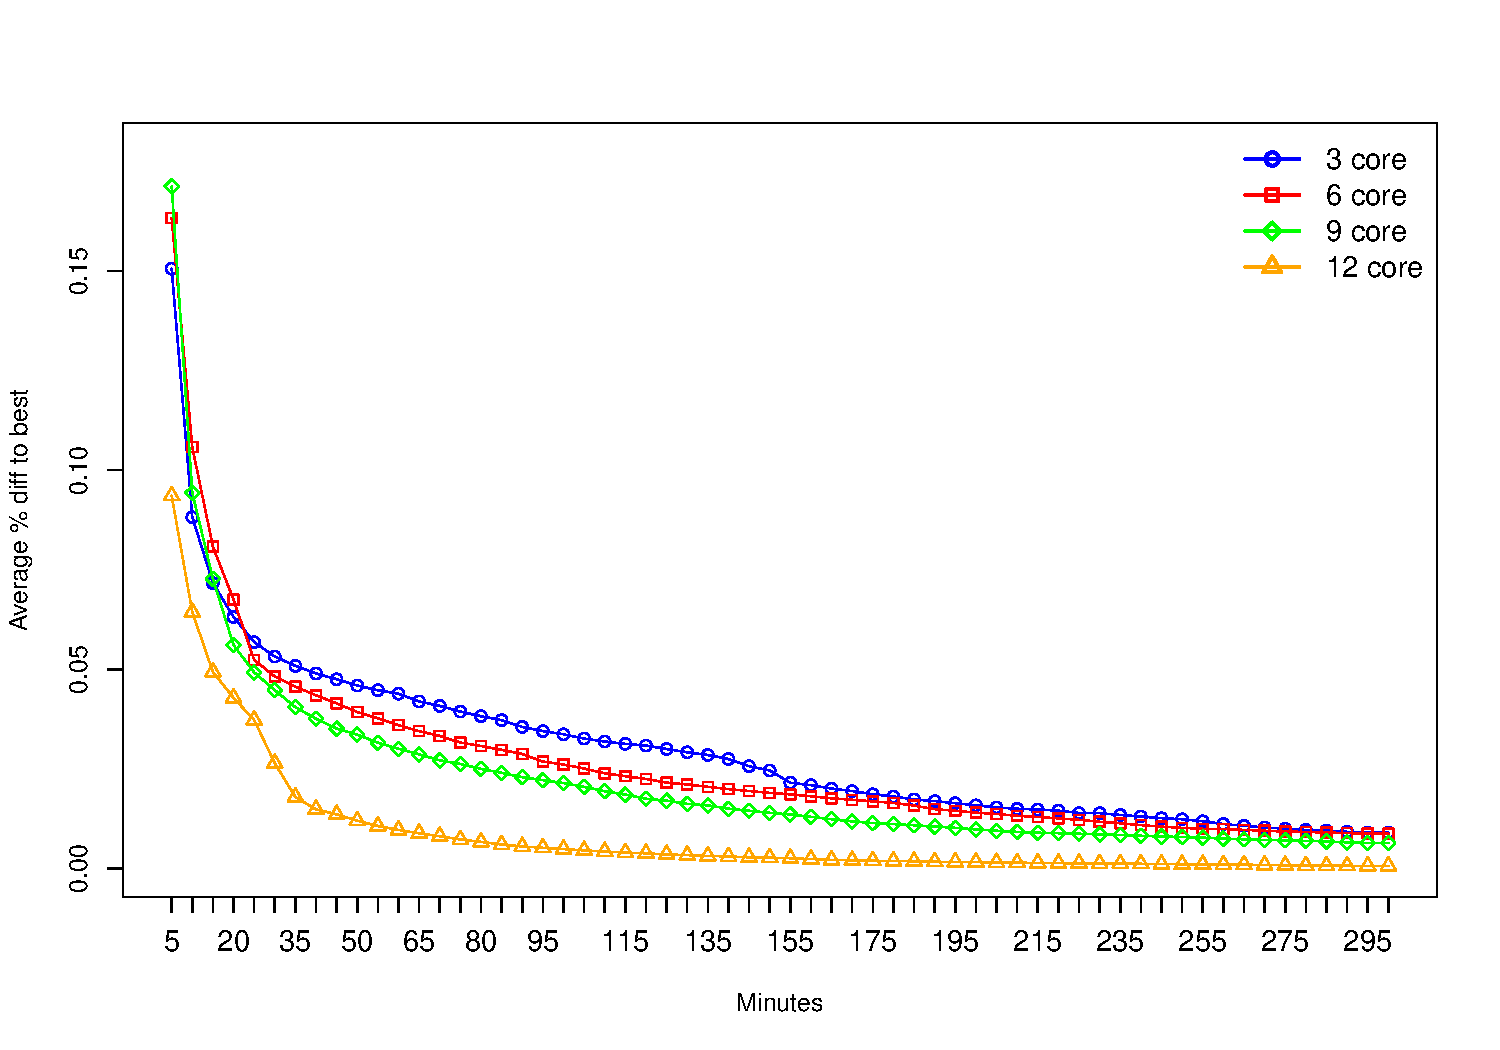
\includegraphics[width=15cm]{CoreConvergenceMS}
  \centering
  \caption{Convergence of P-MS by varying the number of processes (3,6,9,12) for the instances including \emph{Zuck$\_$small, Zuck$\_$medium, Kd, Marvin} and \emph{Sm2}. 
  The y-axis show the gap to the best solution found by all runs across all these instances.}
  \label{fig:concores}
\end{figure}

\subsubsection{Investigating Random Splitting}

\begin{figure}[htbp]
  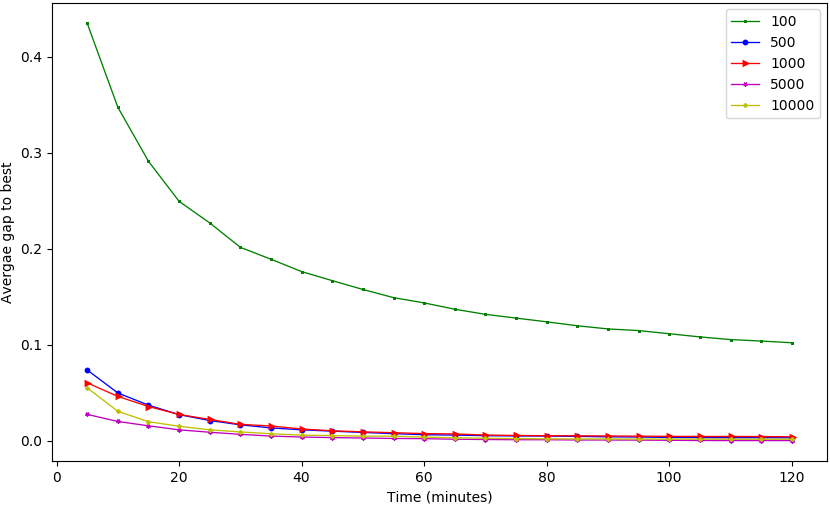
\includegraphics[width=14cm]{kd_ransplit}
  \centering
  \caption{The performance of P-MS on the \emph{Kd} dataset with different levels of random splitting: 100, 500, 1000, 5000, 10000. The y-axis shows the gap to the best solution found across all runs.}
  \label{fig:kd_rs}
\end{figure}

\begin{figure}[htbp]
  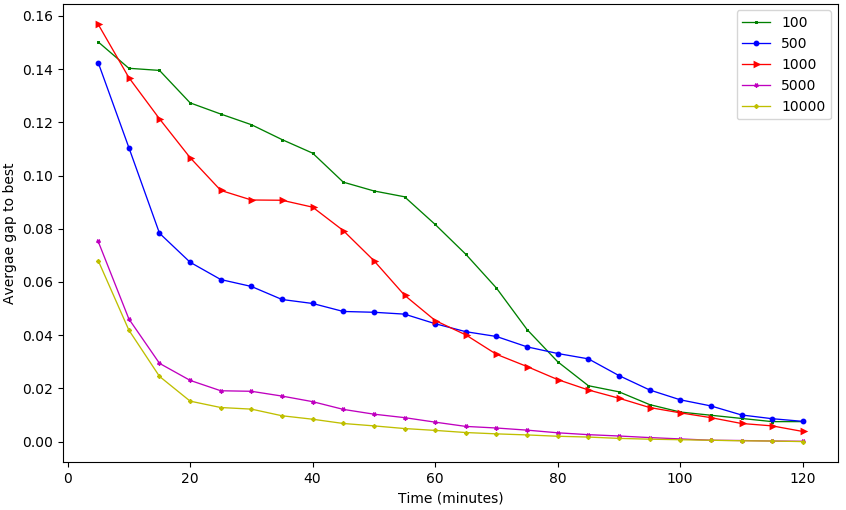
\includegraphics[width=14cm]{marvin_ransplit}
  \centering
  \caption{The performance of P-MS on the \emph{Marvin} dataset with different levels of random splitting: 100, 500, 1000, 5000, 10000. The y-axis shows the gap to the best solution found across all runs.}
  \label{fig:m_rs}
\end{figure}

\begin{figure}[htbp]
  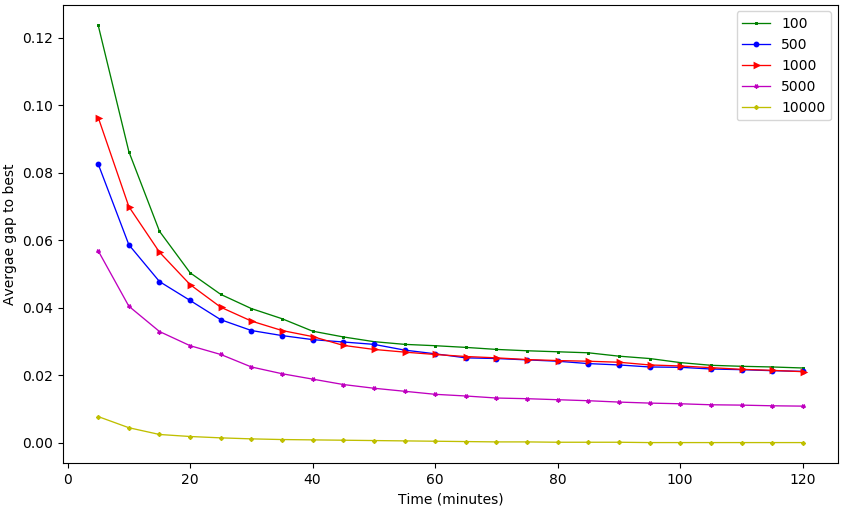
\includegraphics[width=14cm]{zs_ransplit}
  \centering
  \caption{The performance of P-MS on the \emph{Zuck$\_$small} dataset with different levels of random splitting: 100, 500, 1000, 5000, 10000. The y-axis shows the gap to the best solution found across all runs.}
  \label{fig:zs_rs}
\end{figure}

A critical component of MS is random splitting, where too few splits can lead to poor solutions and too many sets render the MILPs intractable. Hence, we investigate the `ideal' amount of random splitting. That is, we wish to identify what level random splitting with lead to the best overall solution and how quickly do the runs converge. For this purpose, we investigate three instances: $Kd$, $Zuck\_small$ and $Marvin$. For each dataset, we consider splitting levels of 100, 500, 1000, 5000 and 10000 sets per iteration. Like the previous experiments, every run was given 12 nodes. Note that the memory requirements increasing substantially with an increase in the number of sets. Hence, splitting beyond 10,000 sets is infeasible, since any further splitting leads to very large memory requirements ($>$ 150 GB) when running 12 instances of MS concurrently.

Figures~\ref{fig:kd_rs}, \ref{fig:m_rs} and \ref{fig:zs_rs} show the results of the experiments of different levels of random splitting. For each dataset, the figures show the progression of the gap of P-MS relative to the best solution found by any of the runs. Like the previous results, initially, more random splitting leads to improved results. Again, this is attributable to a more diverse population directly as a results of considering more sets. Overall, increasing random splitting leads to faster convergence across all datasets. Interestingly, with $Kd$, 5000 sets provide the best result, though 10000 sets also converge nearly as quickly. For all the datasets, 100, 500 and 1000 perform worse than when a larger number of sets are used, but for KD the convergence is a lot more close when using 500 and 1000 sets.

The trend as we see from the random splitting experiments is that increasing diversity is crucial in identifying good solutions. However, the trade-off is with the memory requirements, which for very large problems can be infeasible. This could be the key to achieving much better results for $Zuck\_medium$ and $Zuck\_large$ (i.e., much greater diversity with increased random splitting), which will be a possible direction to investigate in our future work. 

\subsection{Investigating Synchronisation Frequency}

Another aspect of the algorithms that warrants investigation is the regularity of syncing between the nodes (processes). That is, the solutions obtained at each node need to be broadcast to other nodes, and in turn, the receiving nodes need to update the list  of solutions with any better solution information. Synchronisation happens at regular intervals. Here we investigate if syncing within shorter time-periods can lead to better solutions and/or faster convergence.  

\begin{figure}[htbp]
  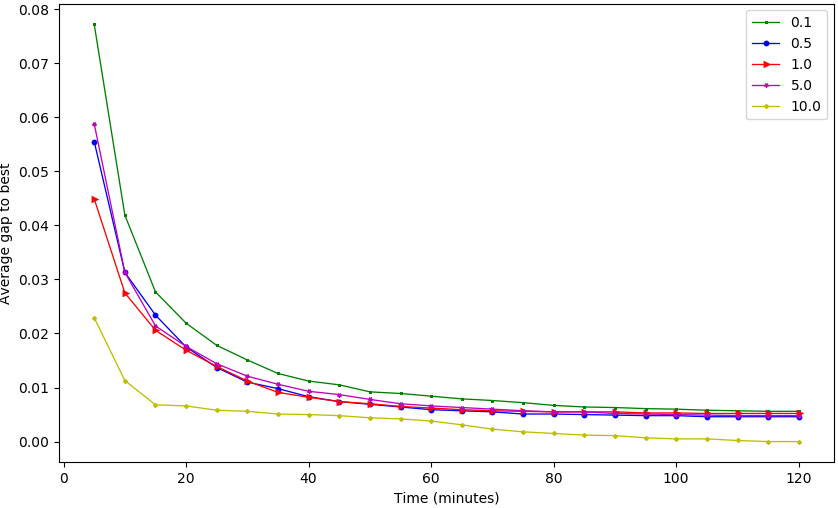
\includegraphics[width=14cm]{kd_sync}
  \centering
  \caption{The performance of P-MS on the Kd dataset with different syncing times (in seconds): 0.1, 0.5, 1.0, 5.0, 10.0. The y-axis show the gap to the best solution found by all runs across.}
  \label{fig:kd_sync}
\end{figure}

\begin{figure}[htbp]
  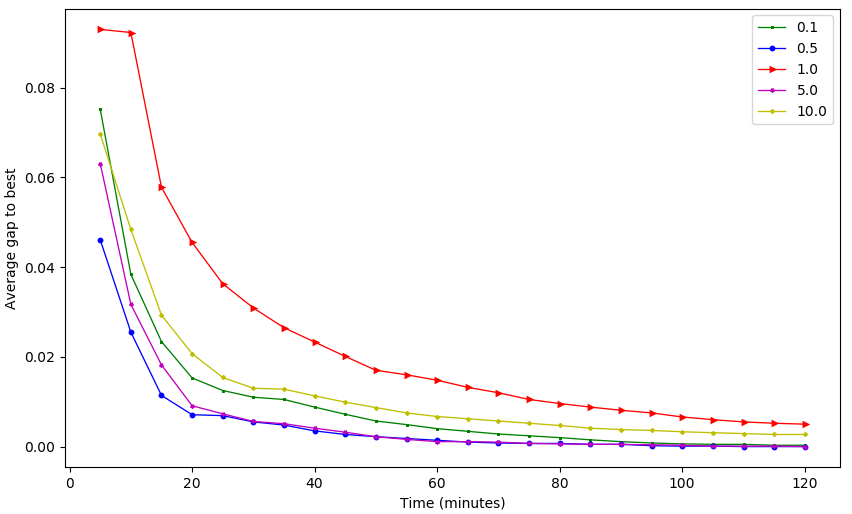
\includegraphics[width=14cm]{marvin_sync}
  \centering
  \caption{The performance of P-MS on the Marvin dataset with different syncing times (in seconds): 0.1, 0.5, 1.0, 5.0, 10.0. The y-axis show the gap to the best solution found by all runs across.}
  \label{fig:m_sync}
\end{figure}

\begin{figure}[htbp]
  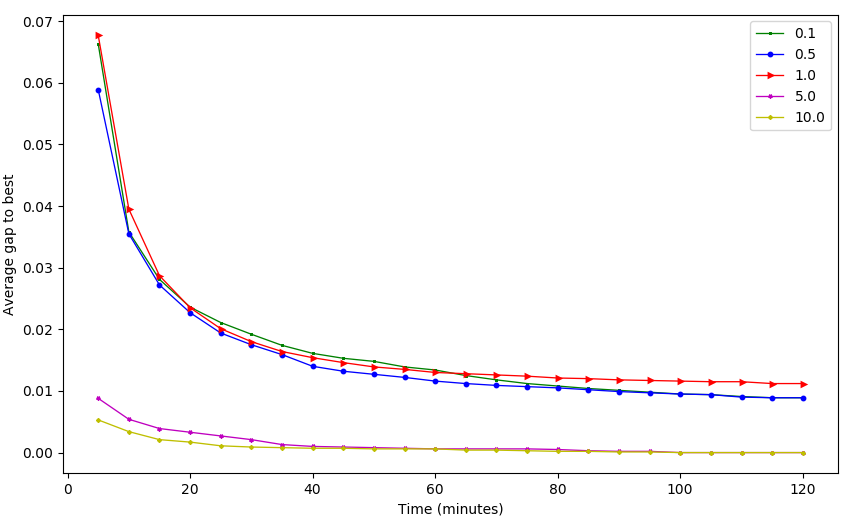
\includegraphics[width=14cm]{zs_sync}
  \centering
  \caption{The performance of P-MS on the Zuck$\_$small dataset with different syncing times (in seconds): 0.1, 0.5, 1.0, 5.0, 10.0. The y-axis show the gap to the best solution found by all runs across.}
  \label{fig:zs_sync}
\end{figure}

Like the previous section, we investigate P-MS on the Kd, Marvin and $Zuck\_small$ datasets. Figures~\ref{fig:kd_sync}, ~\ref{fig:m_sync} and ~\ref{fig:zs_sync} show the results for each of these datasets, respectively. The figures show the gap to the best solution (found by any of the runs) for 120 minutes. The syncing times considered are 0.1, 0.5, 1.0, 5.0 and 10 seconds. 

The results in these figures show that there are advantages with respect to solution quality and convergence rate. For Kd, we see that syncing too often ($\leq$ 5 seconds) is not useful and 10 or more seconds is beneficial. However, for Marvin, syncing at 0.5 or 5 seconds works well. Like, Kd, there is a distinct advantage for larger sync times ($\geq$ 5 seconds) for $Zuck\_small$.  The Marvin dataset consists of many more blocks and precedence constraints than Kd or $Zuck\_small$, and there are also many more solution improvements generated during the course of a run. Hence, these results show that if the starting solution is poor or far away from a local or global optimal solution, syncing often can lead to finding better solutions and a faster rate of convergence.

\section{Conclusion}\label{sec:conc}
This study investigates open pit mining, a complex optimisation problem arising in the mining industry. The problem instances can be very large with over 100,000 blocks and 1 million precedence constraints. Hence, to find good solutions in reasonable times, we propose a novel distributed approach -- parallel Merge Search. The key idea behind this method is its ability to combine large populations of solutions (via variable aggregation). When applied in a distributed setting, the approach proves to be very effective. We also implement a depth first Branch \& Bound approach with the aim of finding good upper bounds.

We see that Merge Search on its own finds very good solutions to known benchmark instances of open pit mining, finding better solutions on four out of seven instances. Furthermore, its parallel implementation (via MPI) proves to be the best performing method, finding best known solutions in five out of seven problem instances. On investigating its convergence characteristics, we see that solution diversity is crucial in achieving good performance. The Branch \& Bound approach, while not able to find the best heuristic solutions, has produced the best known upper bounds for all the problem instances. 

\subsection{Future Work}

Diversity in the solution population is key part of ensuring that Merge Search is implemented efficiently. Moreover, it is very flexible with the ability to combine solutions from different approaches (like heuristics, meta-heuristics, exact methods, etc.) easily. Combining these aspects, Merge Search - heuristic/meta-heuristic hybrids can be expected to achieve superior performance compared to Merge Search on its own. Hence, for future work, we are extending Merge Search for open pit mining in this direction, where we are developing hybrids with  ant colony optimisation~\citep{dorigo04}, particle swarm optimisation~\citep{Kennedy95} and scheduling heuristics~\citep{Thiruvady2013}. The diversity achieved from these approaches and the ability to implement all them in a fully parallel setting, is likely to provide substantial improvements in solution quality and quicker convergence in terms of wall-clock time. 

The generic nature of Merge Search means that it can be easily applied to other problems. Several optimisation problems have different solution approaches, for example, those derived from heuristics, meta-heuristics, constraint programming \citep{marriott98}, etc. Merge Search can be used to efficiently combine the solutions found by these methods, and will be particularly advantageous for very large problems. In fact, Merge Search is proven on the constrained pit mining problem \citep{Kenny:2018} and we have conducted preliminary studies that show that it can be applied to resource constrained job scheduling \citep{singhernst10} and resource constrained project scheduling \citep{kimms00}.

A key motivation for the development of Merge Search was distributed processing. The parallel MPI framework proposed here can be further extended to consider a very large number of nodes, which will present its own challenges. It can be expected that by carefully designing the hybrids, very large improvements can be achieved. Parallelisation via a shared memory architectures could also be of great potential. For example, within a node, individual metaheuristic methods could be implemented in parallel (e.g. multiple solutions constructed in parallel in ACO ~\citep{Thiruvady14a,ernst_hybrid_2010}).  

 
\appendix

\section{Network Flow Structure}\label{sec:network_flow}

Consider the problem without resource constraints~\eqref{eq:resource}. Firstly,
in this case the optimal solution is simply to use the more profitable option
for each block $b$ so 
$$y_{b\bar dt}=\left \{ \begin{array}{ll}
                \bx_{bt}-\bx_{b,t-1} & \hbox{if }  \bar d=\argmax_{d\in D}p_{bdt}\\
                0 & \hbox{otherwise}
               \end{array} \right.
               $$
Hence, the problem reduces to one of maximising over $\bx$
variables with profit $\bar p_{bt} = p_{b\bar dt}-p_{b,\bar d,t+1}$.
Hence, in general, since constraints \eqref{eq:once} have the same structure as
\eqref{eq:prec} we can simply consider variables $\bx_i$ where $i=(b,t)\in N$ and
precedence relationship $(i,j)\in\mathcal{P}$ where either $i=(a,t)$ and
$j=(b,t)$ with $a\rightarrow b$ or $i=(b,t+1)$ and $j=(b,t)$. That is, the
predecessors for block $b$ at time $t$ are the blocks $a$ ``above'' $b$ and
the block $b$ at the next time period $t$. Using the notation $p_i$ to denote
the arbitrary profit of $i$ we get:
\begin{alignat}{3}   %% number of &'s = 2 * cols - 1
  \noalign{\noindent\bf Problem P}
  %% alignment is right, left, right, left, ....
  &&\max\quad&\sum_{i\in N} p_i\,\bx_i   & \label{eq:Pobj}\\
  \text{s.t. } && \bx_j - \bx_i &\,\leq\, 0&&\forall\ i\rightarrow j  \label{eq:Pprec}\\ 
  && \bx_i &\,\leq\, 1&& \forall\ i\in N\label{eq:Pbxle1}\\
  && \bx_i &\,\geq\, 0&& \forall\ i\in N\label{eq:Pxge0}
\end{alignat}
Note that we really only require \eqref{eq:Pbxle1} for a significantly reduced set
$N^{0}\subseteq N$ that have no predecessors. So this might means all of the
nodes corresponding to the last time period and blocks at the top of the open cut mine.
The optimal solution to this problem is a set $C\subseteq N$ of nodes to be
selected such that all arcs in the cut point out of $C$ ($i\in C$ and $j\rightarrow i$
$\Rightarrow$ $j\in C$) which maximises $\sum_{i\in C} p_i$.

Let $\phi_{ij}$ be the dual variable associated with \eqref{eq:Pprec} and
$\mu_i$ correspond to \eqref{eq:Pbxle1} then the dual problem is:
\begin{alignat}{3}   %% number of &'s = 2 * cols - 1
  \noalign{\noindent\bf Problem D}
  %% alignment is right, left, right, left, ....
  &&\min\quad&\sum_{i\in N^0} \mu_i   & \label{eq:Pobj_1}\\
  \text{s.t.} && \sum_{j:i\rightarrow j} \phi_{ij} -
  \sum_{j:j\rightarrow i} \phi_{ji} -\mu_i&\,\leq\, -p_i &\quad&\forall\ i\in N \label{eq:Dflow}\\ 
  && \phi_{ij},\ \mu_i &\,\geq\, 0&& \forall\ i,j\in N\label{eq:Dge0}
\end{alignat}
Note that we have multiplied \eqref{eq:Dflow} by $-1$ to make it clearer that
this is a standard network flow equation where the net outflow (sum of
$\phi_{ij}$ going out of $i$ minus what is coming in via arcs pointing into $i$
and $\mu_i$) must be at most the `production' amount $-p_i$. In other words
this is a network flow problem with the following characteristics:
\begin{itemize}
\item Any node can ``discard'' flow but each node can produce at most $-p_i$.
  Where $-p_i < 0$ (i.e., positive profit in Problem P), the node has a minimum
  amount of net flow $p_i$ that needs to be provided (go into node $i$).
\item Flow can be moved at no cost and with no capacity restrictions between
  nodes but only along the precedence arcs $i\rightarrow j$.
\item A ``dummy'' node can be used to make up any shortfall $\mu_i$ at unit
  cost. That is, we are minimising the total shortfall after any supply is used
  to meet demand.
\end{itemize}
Alternatively we can think of this as a maximum flow problem where
\begin{itemize}
\item We start with the basic network defined by the $i\rightarrow j$ arcs and
  add a source $\alpha$  and sink node $\omega$.
\item Each node $i$ for which $-p_i > 0$ (i.e. a loss in our original
  problem) we create an arc from the source node to $i$ ($\alpha\rightarrow i$) with capacity $-p_i$.
\item For all other nodes $p_i \geq 0$ we add an arc from $i$ to a sink
  ($i\rightarrow \omega$) with capacity $p_i$.
\item Maximising the flow gives an optimal solution $f^{max}$ such that
  $\sum_{i:p_i>0} p_i - f^{max}$ equals the optimal solution value of Problems
  $P$ and $D$ and the corresponding optimal cut matches (is the complement of)
  the optimal cut of $C$.
\end{itemize}

\section{Incremental destination variables}\label{sec:incremental}
If we define the amount sent to destinations incrementally we obtain the cumulative variables $\by_{bdt}$. These specify the amount of flow that has been sent to any destination
  before time $t$, or to a higher indexed destination $d$ during $t$:
  $$\by_{bdt} = \sum_{\tau < t}\sum_{\delta\in D} y_{b\delta\tau} +
  \sum_{\delta \geq d} y_{b\delta t}$$  
Note that now $\bx_{bt}=\by_{b0t}$.  Also in our data sets we have only
two destinations with $\by_{b0t}$ being the total amount mined (irrespective
of destination) and $\by_{b1t}$ the amount sent to be processed (destination
1) for block $b$ by time $t$.

To simplify the presentation and match the notation for block predecessors we
define a ``predecessor'' (really later in time or lower indexed destination) relationship with
$(d,t)\rightarrow (\delta,\tau)$ if
$$ d=\delta-1 \land t=\tau; \text{ or } \delta=0 \land d=|D|-1 \land t
>\tau.$$
It can be seen that here $(\delta,\tau)$ is really a unique ``successor'' to $(d,t)$.
Also we have $y_{bdt} = \by_{bdt}-\by_{b,d',t'}$ where
$(d,t)\rightarrow(d',t')$ is the predecessor. Using these new variables and expanded precedence relationships we obtain a new formulation for problem PCPSP:
\begin{alignat}{3}   %% number of &'s = 2 * cols - 1
%  \noalign{\noindent\bf Problem PCPSP}
  %% alignment is right, left, right, left, ....
  &&\max\quad&\sum_{b\in B}\sum_{d\in D}\sum_{t\in T} \bar p_{bdt}\,\bar y_{bdt}   & \label{eq:yobj}\\
  \text{s.t.} && \by_{b0t} &\,\leq\, \by_{a0t}&&\forall\ (a,b)\in\mathcal{P},\ t\in T  \label{eq:yprec}\\ 
  && \by_{bd't'} &\,\leq\, \by_{bdt} && \forall\ b\in B,\ d\in D,\ t\in T,
  \text{ if }(d,t)\rightarrow(d',t') \label{eq:yincr}\\
  &&\sum_{b\in B}\sum_{d\in D} q_{bdr}\,\left(
    \by_{bdt}-\by_{bd't'}|_{(d,t)\rightarrow(d',t')}
  \right)&\,\leq\, \bar R_{rt}&&\forall\  r\in R,\ t\in T\label{eq:yresource}\\
  &&\by_{b0t}\in\{0,1\}, 0\leq \by_{bdt}&\,\leq\, 1
  &&\forall\ b\in B,\ d\in D,\ t\in T \label{eq:yvars}
\end{alignat}
This has just precedence ($\leq$) style constraints plus resource
constraints similar to the formulation based on $\bx$ above. 
Here $\bar p_{bdt}=p_{bdt}-p_{bd't'}$ where $(d',t')\rightarrow(d,t)$ to
ensure we get the right cost.
As for the previous formulation, we only need $\by_{b,0,0}\geq0$ and
$\by_{b,D,T}\leq 1$ with all other bounds on $\by_{b,d,t}$ variables implied
by the relationship \eqref{eq:yincr}.

\section{Aggregation Formulation}\label{sec:agg}
Let $S$ be a set of $(b,d,t)$ triplets and $\by_{S}$ be a corresponding
variable that indicates that all $\by_{bdt}$ have the same value $\by_S$.
Assume we have a collection of such sets $\mathcal{S}$ that is the union of
one or more partitions of the set $\mathcal{N}$ of all such triplets.
Typically, we are only interested in connected subsets of $\mathcal{N}$ (by the
precedence and predecessor arcs $\rightarrow$). In particular, we have special cases:
\begin{itemize}
\item $\mathcal{S}=\left\{\ \{(b,d,t)\} \mid (b,d,t)\in \mathcal{N}\right\}$ where the
  $\by_{S}$  variables are identical to the original $\by_{bdt}$ variables.
\item $\mathcal{S}=2^{\mathcal{N}}$ where every connected subset of
  $\mathcal{N}$ is included (of theoretical interest only).
\item Some non-trivial partition of $\mathcal{N}$ leading to a column
  generation master problem that may or may not have the same optimal solution
  as our original problem. 
\end{itemize}
We want to set up this kind of master problem and incrementally refine the
partition to get the optimal solution to the LP relaxation of our problem.
To enable a compact definition of this formulation we define:
\begin{description}
\item[$B(S)$] the set of blocks for which some triplet $(b,d,t)\in S$ so that
  $B(S)\subseteq B$.
\item[$\alpha(b,S),\omega(b,S)$] $\alpha(b,S)$ the first triplet not in $S$
  and the last triplet in $S$ of the chain involving block $b$. That is, assume
  that we have:
  $$\alpha(b,S)=(b,d_0,t_0)\rightarrow (b,d_1,t_1) \rightarrow \ldots
  \rightarrow (b,d_k,t_k)=\omega(b,S)$$
  Then $(b,d_0,t_0)\not\in S$, and $(b,d_i,t_i)\in S$ for $i=1,\ldots,k$.
  \begin{itemize}
  \item Alternative ways to set up these chains are possible, but we use the same ordering as for the incremental formulation described in Section~\ref{sec:incremental}.
  \item $\alpha(b,S)$ may not exist - $S$ may contain the first triplet for a
  block. This just means that in the sums below, the corresponding constant is
  not included.
  \end{itemize}
\item[$S\rightarrow S'$] if $\exists (b,d,t)\in S,(b',d',t')\in S' :
  (b,d,t)\rightarrow(b',d',t') $\\
  With this definition it is possible to have $S\rightarrow S'$ and
  $S'\rightarrow S$. We restrict ourselves to only consider partitions $\cal S$ where this does not occur. 
\item[$\bar p_{S}$] The total profit due to all $(b,d,t)\in S$:
  $$\bar p_{S}=\sum_{(b,d,t)\in S} \bar p_{bdt}
  = \sum_{b\in B(S)} p_{b\omega(b,S)} - p_{b\alpha(b,S)}
  $$
\item[$\bar q_{Srt}$] the amount of resource $r$ consumed in $t$ if we select
  all nodes in $S$.
  $$\bar q_{Srt}=\sum_{b,d:(b,d,t)\in S} \bar q_{b,d,t}
  =\sum_{b,d:\omega(b,S)=(d,t)} q_{b,d,t} - \sum_{b,d:\alpha(b,S)=(d,t)} q_{b,d,t}$$
\end{description}
\begin{alignat}{3}   %% number of &'s = 2 * cols - 1
  \noalign{\noindent\bf Problem PCPSP($\mathcal{S}$)}
  %% alignment is right, left, right, left, ....
  &&\max\quad&\sum_{S\in \mathcal{S}} \bar p_{S}\,\by_S   & \label{eq:Sobj}\\
  \text{s.t.} && \by_{S'} &\,\leq\, \by_{S}&&
  \forall\ S\rightarrow S'\in\mathcal{S} \label{eq:Sprec}\\ 
  &&\sum_{S\in\mathcal{S}} q_{Srt}\by_S&\,\leq\, \bar R_{rt}&&\forall\  r\in R,\ t\in T\label{eq:Sresource}\\
  && 0\,\leq\, \by_{S}&\,\leq\, 1  &&\forall\ S\in\mathcal{S} \label{eq:Svars}\\
  && \by_S&\,\in\,\{0,1\}&&\forall\ S\in\mathcal{S}:\exists (b,0,t)\in S
\end{alignat}
Any solution to PCPSP$(\mathcal{S})$ clearly corresponds to a primal feasible
solution of the original PCPSP (with all of the $\by_{bdt}$ set according to
the corresponding $\by_S$). To prove that a solution is \emph{optimal} we need
to ensure dual feasibility. That is, we need to ensure we have a way of
assigning dual variables (flows) for all of the internal edges that have been
dropped by using the aggregation $\mathcal{S}$. For a particular
$S\in\mathcal{S}$ this means we need a feasible solution to a flow problem
with supply equal to the negative of reduced costs based on duals of
$\lambda_{rt}$ of \eqref{eq:Sresource}. Thus supply $\sigma_{bdt}$ is given by:
\begin{equation} \label{eq:Ssupply}
  \sigma_{bdt}=-\bar p_{bdt} -
  \sum_{rt:\omega(b,S)=(d,t)}\lambda_{rt}q_{bdt}%%\big|_{\omega(b,S)=(d,t)}
  +\sum_{rt:\alpha(b,S)=(d,t)} \lambda_{rt}q_{bdt}%%\big|_{\alpha(b,S)=(d,t)}
\end{equation}
In addition, we introduce dummy supply nodes $S'$ for all other sets
$S'\ne S\in\mathcal{S}$ with supply $\phi_{S'S}$ (dual of \eqref{eq:Sprec}
where $S'\rightarrow S$) and arcs
$S'\rightarrow(b,d,t)$ if $\exists (b',d',t')\in
S':(b',d',t')\rightarrow(b,d,t)\in S$. Also, potentially dummy sink nodes $S''$
for any set $S''\in\mathcal{S}$ with supply $-\phi_{SS''}$  (dual of
\eqref{eq:Sprec} where $S\rightarrow S''$) and arcs $(b,d,t)\rightarrow S''$ if
$\exists (b'',d'',t'')\in S'':(b,d,t)\rightarrow{}(b'',d'',t'')$.
Note that we can in principle check this feasibility by solving max flow from
the dummy source to dummy sink nodes (with arcs limited by $\phi$). If this
produces a cut with all of the $(b,d,t)\in S$ on the same side of the cut (i.e.,
we are just cutting off the source or sink nodes) then the solution is dual
feasible, otherwise we have a way of partitioning $S$ into two subsets which
could lead to an improvement of the solution. This forms the basis for the Bienstock-Zuckerberg Algorithm.

%\subsection{Bienstock \& Zuckerberg}\label{sec:bz}
%The LP relaxation of the PCPSP is solved using the Bienstock--Zuckerberg algorithm ~\citep{zuckerberg2010} which has been developed for the LP relaxation of 
%large scale precedence constrained production scheduling problems. Lagrangian relaxation is used to solve the linear program by dualizing the resource 
%constraints. In each iteration, the Lagrangian multipliers are updated using the optimal dual values of the resource constraints in restricted version of 
%the LP relaxation, where variables are aggregated with respect to the partitions constructed using the max closure in each iteration of the approach. The 
%algorithm is presented in Algorithm~\ref{alg:bz}. Note that this algorithm iterates between finding valid upper (relaxed) bounds via Lagrangian relaxation 
%and valid LP lower bounds (feasible fractional solutions) by solving restricted LPs. The restricted LPs simply require that for any pair of 
%variables (corresponding to block,destination,time triplets) that have had the same solution value in each of the 
%Lagrangian iterations so far, then they must also take the same value in the LP (See Step~\ref{step:aggregate} of Algorithm~\ref{alg:bz}).  For more 
%details see~\cite{zuckerberg2010}. 

%First $x$ variables are removed from the formulation PCPSP. Then the problem is reformulated in terms of new variables defined as
%\begin{equation}
% z_{btd} = \sum_{\tau =1}^{t-1} \sum_{\eta=1}^{d_{max}} y_{b\tau \eta} + \sum_{\eta=1}^{d} y_{bt \eta} 
%\end{equation}
%for all $b \in B, t \in [1, t_{max}], d \in [1, d_{max}] $.

%\begin{eqnarray}
% \max && \sum_{b\in B} \sum_{t=1}^{t_{max}} \sum_{d=2}^{d_{max}} p_{btd} (z_{btd} - z_{bt,d-1}) + \label{eq:BZ:obj}\\
% &&\hspace{10ex}  + \sum_{b\in B} \sum_{t=2}^{t_{max}} p_{bt1} (z_{bt1} -
%    z_{b,t-1,d_{max}})+
    % \\ &&\hspace{10ex}  +
%   \sum_{b\in B} p_{b,1,1} z_{b,1,1}\\
% \hbox{s.t.} && z_{a,t,d_{max}}\leq z_{b,t,d_{max}}  \hspace{10ex} \forall a \in B, \forall b \in P(a), \forall t \in [1, t_{max}] \\
% && z_{bt_{max}d_{max}}\leq 1 \hspace{10ex} \forall b \in B\\
% && z_{bt,d-1}\leq z_{btd}  \hspace{10ex} \forall b \in B, \forall t \in [1, t_{max}], \forall d \in [2, d_{max}]\\
% && z_{b,t-1,d_{max}}\leq z_{bt1}  \hspace{10ex} \forall b \in B, \forall t \in [2, t_{max}]\\
% && \underline{R}_{rt} \leq \sum_{b\in B}\sum_{d=2}^{d_{max}} q_{bdr}(z_{btd} - z_{bt,d-1}) + \sum_{b\in B}q_{b1r}(z_{bt1} - z_{b,t-1,d_{max}}) \leq \overline{R}_{rt} \label{eqn:BZ:R}\\
% &&\hspace{30ex} \forall r \in [1, r_{max}],  \forall t \in [2, t_{max}]\nonumber\\
% && \underline{R}_{r1} \leq \sum_{b\in B}\sum_{d=2}^{d_{max}} q_{bdr}(z_{b1d} - z_{b1,d-1}) + \sum_{b\in B}q_{b1r}z_{b11} \leq \overline{R}_{r1}\label{eqn:BZ:R2} \\
% && \hspace{30ex} \forall r \in [1, r_{max}]\nonumber\\
% && z_{btd} \geq 0   \hspace{10ex} \forall b \in B, \forall t \in [1, t_{max}], \forall d \in [1, d_{max}] \label{eq:BZ:bounds}
% \end{eqnarray}
 
%% For each variable $z_{btd}$, the objective coefficient is defined as follows
%% \begin{equation}
%% p_{btd} - \left \{ \begin{array}{ll}
%%                        p_{bt,d+1} & if \ d < d_{max}\\
%%                        p_{b,t+1,1} & if \ d = d_{max}, \; t<t_{max}\\
%%                        0 & otherwise( d = d_{max}, \; t=t_{max})
%%                       \end{array} \right .
%% \end{equation}
%% For Lagrangian relaxation of the problem, i.e. when the resource constraints are dualized, the objective coefficients 
%% are
%% \begin{eqnarray*}
%%  c_{btd} & = & p_{btd} - \left \{ \begin{array}{ll}
%%                                0 & \hbox{if } d= d_{max}, t=t_{max}\\
%%                                p_{b,t+1,1} & \hbox{if } d=d_{max}, t < t_{max}\\
%%                                p_{bt,d+1} & \hbox{if } d < d_{max}
%%                               \end{array} \right .\\
%%          & &\color{blue} - \left \{ \begin{array}{ll}
%%                                0 & \hbox{if } d= d_{max}, t=t_{max}\\
%%                                \sum_{r=1}^{r_{max}} \bar{\lambda}_{tr} q_{bdr} & \hbox{otherwise}
%%                               \end{array} \right .\\
%%          & &\color{blue} + \left \{ \begin{array}{ll}
%%                                0 & \hbox{if } t=t_{max} \ \hbox{and } d=1 \ \hbox{or } d_{max}\\
%%                                \sum_{r=1}^{r_{max}} \bar{\lambda}_{tr} q_{b,d+1,r} & \hbox{if } d \not = d_{max} \ \hbox{and } !(d=1, t=t_{max}) \\
%%                                \sum_{r=1}^{r_{max}} \bar{\lambda}_{t+1, r} q_{b1r} & \hbox{if } d = d_{max}, t<t_{max} 
%%                               \end{array} \right .\\
%%          & & \color{green} + \left \{ \begin{array}{ll}
%%                                0 & \hbox{if } d= d_{max}, t=t_{max}\\
%%                                \sum_{r=1}^{r_{max}} \underline{\lambda}_{tr} q_{bdr} & \hbox{otherwise}
%%                               \end{array} \right .\\
%%          & & \color{green}- \left \{ \begin{array}{ll}
%%                                0 & \hbox{if } t=t_{max} \ \hbox{and } d=1 \ \hbox{or } d_{max}\\
%%                                \sum_{r=1}^{r_{max}} \underline{\lambda}_{tr} q_{b,d+1,r} & \hbox{if } d \not = d_{max} \ \hbox{and } !(d=1, t=t_{max}) \\
%%                                \sum_{r=1}^{r_{max}} \underline{\lambda}_{t+1, r} q_{b1r} & \hbox{if } d = d_{max}, t<t_{max} 
%%                               \end{array} \right .                              
%% \end{eqnarray*}
\section*{Acknowledgements}
 This research was supported in part by the Monash eResearch Centre and eSolutions-Research Support Services through the use of the MonARCH HPC Cluster.
\section*{References}
\bibliography{references}
\end{document}
